% Options for packages loaded elsewhere
\PassOptionsToPackage{unicode}{hyperref}
\PassOptionsToPackage{hyphens}{url}
\PassOptionsToPackage{dvipsnames,svgnames,x11names}{xcolor}
%
\documentclass[
  11pt,
]{book}
\title{Local SDGs systems model documentation}
\author{Katrina Szetey, Enayat A. Moallemi, Brett A. Bryan}
\date{February 2022}

\usepackage{amsmath,amssymb}
\usepackage{lmodern}
\usepackage{iftex}
\ifPDFTeX
  \usepackage[T1]{fontenc}
  \usepackage[utf8]{inputenc}
  \usepackage{textcomp} % provide euro and other symbols
\else % if luatex or xetex
  \usepackage{unicode-math}
  \defaultfontfeatures{Scale=MatchLowercase}
  \defaultfontfeatures[\rmfamily]{Ligatures=TeX,Scale=1}
\fi
% Use upquote if available, for straight quotes in verbatim environments
\IfFileExists{upquote.sty}{\usepackage{upquote}}{}
\IfFileExists{microtype.sty}{% use microtype if available
  \usepackage[]{microtype}
  \UseMicrotypeSet[protrusion]{basicmath} % disable protrusion for tt fonts
}{}
\makeatletter
\@ifundefined{KOMAClassName}{% if non-KOMA class
  \IfFileExists{parskip.sty}{%
    \usepackage{parskip}
  }{% else
    \setlength{\parindent}{0pt}
    \setlength{\parskip}{6pt plus 2pt minus 1pt}}
}{% if KOMA class
  \KOMAoptions{parskip=half}}
\makeatother
\usepackage{xcolor}
\IfFileExists{xurl.sty}{\usepackage{xurl}}{} % add URL line breaks if available
\IfFileExists{bookmark.sty}{\usepackage{bookmark}}{\usepackage{hyperref}}
\hypersetup{
  pdftitle={Local SDGs systems model documentation},
  pdfauthor={Katrina Szetey, Enayat A. Moallemi, Brett A. Bryan},
  colorlinks=true,
  linkcolor={Maroon},
  filecolor={Maroon},
  citecolor={Blue},
  urlcolor={blue},
  pdfcreator={LaTeX via pandoc}}
\urlstyle{same} % disable monospaced font for URLs
\usepackage[left=3cm, right=3cm, top=2.5cm, bottom=2.5cm]{geometry}
\usepackage{longtable,booktabs,array}
\usepackage{calc} % for calculating minipage widths
% Correct order of tables after \paragraph or \subparagraph
\usepackage{etoolbox}
\makeatletter
\patchcmd\longtable{\par}{\if@noskipsec\mbox{}\fi\par}{}{}
\makeatother
% Allow footnotes in longtable head/foot
\IfFileExists{footnotehyper.sty}{\usepackage{footnotehyper}}{\usepackage{footnote}}
\makesavenoteenv{longtable}
\usepackage{graphicx}
\makeatletter
\def\maxwidth{\ifdim\Gin@nat@width>\linewidth\linewidth\else\Gin@nat@width\fi}
\def\maxheight{\ifdim\Gin@nat@height>\textheight\textheight\else\Gin@nat@height\fi}
\makeatother
% Scale images if necessary, so that they will not overflow the page
% margins by default, and it is still possible to overwrite the defaults
% using explicit options in \includegraphics[width, height, ...]{}
\setkeys{Gin}{width=\maxwidth,height=\maxheight,keepaspectratio}
% Set default figure placement to htbp
\makeatletter
\def\fps@figure{htbp}
\makeatother
\setlength{\emergencystretch}{3em} % prevent overfull lines
\providecommand{\tightlist}{%
  \setlength{\itemsep}{0pt}\setlength{\parskip}{0pt}}
\setcounter{secnumdepth}{1}
\usepackage[none]{hyphenat}
\raggedbottom 
\ifLuaTeX
  \usepackage{selnolig}  % disable illegal ligatures
\fi
\usepackage[]{natbib}
\bibliographystyle{apalike}

\begin{document}
\maketitle

{
\hypersetup{linkcolor=}
\setcounter{tocdepth}{1}
\tableofcontents
}
\hypertarget{introduction}{%
\chapter*{Introduction}\label{introduction}}
\addcontentsline{toc}{chapter}{Introduction}

\hypertarget{local-sdgs-systems-model}{%
\section*{Local SDGs systems model}\label{local-sdgs-systems-model}}
\addcontentsline{toc}{section}{Local SDGs systems model}

This document is the complete model documentation for the Local SDGs systems model, designed by Katrina Szetey, Enayat A. Moallemi, Brett A. Bryan, and the people of Forrest, Victoria, Australia. The model describes the system of Forrest in the context of sustainability achievement and the Sustainable Development Goals.

The model contains twelve \emph{model components}, and this document is arranged with one chapter for each of those components. There is an overview of the component, a stating of \emph{problem definitions}, and \emph{dynamic hypotheses} that explain how each problem has emerged. There is a description of the system conceptualisation for each component, and a diagram of a conceptual model (excepting for the Climate Change component). Data sources are listed and links to code and data in Github are provided. The final section of each chapter is a listing of every variable in the model component, stating variable type, formula, units, and any assumptions and data that were used in formulating the variable. References are listed at the end of the document.

\hypertarget{demographic-component}{%
\chapter{Demographic component}\label{demographic-component}}

Forrest has been a regional Victorian township since 1890 and developed around the railway built to transport Otway timber and produce. The population has waxed and waned with its timber and forestry activities, at a peak in the 1960s. With tourism having replaced forestry as the primary economic activity in Forrest, this too may result in volatility in population (especially with the impact on tourism from the Covid-19 pandemic).

\hypertarget{problem-definition}{%
\section{\texorpdfstring{\emph{Problem definition}}{Problem definition}}\label{problem-definition}}

\begin{enumerate}
\def\labelenumi{\arabic{enumi}.}
\tightlist
\item
  Between 2006 and 2016, Forrest experienced a 35\% increase in population. Over that time, the number of children aged 0-14 decreased by 14\% and people over 55 increased by 26\%. The median age of a person living in Forrest has increased from 41 to 52. Forrest has a slowly increasing and ageing population, which will influence the needs of residents in the future.
\end{enumerate}

\emph{Dynamic hypothesis:}
The population in Forrest is ageing due to in-migration of couples without children, and out-migration of young people for school and work after they finish high school. It is limited by housing availability and a lack of diversity in job opportunities.

\begin{enumerate}
\def\labelenumi{\arabic{enumi}.}
\setcounter{enumi}{1}
\tightlist
\item
  With Forrest Primary School being the central school, pre-school, and childcare service for the community and neighbouring townships, it creates traffic for local businesses in town. It also works with many of the community groups in Forrest. If Forrest were to lose its primary school, there would be many negative knock-on effects causing harm to Forrest's future, such as out-migration of families seeking access to closer schools.
\end{enumerate}

\emph{Dynamic hypothesis:}
The location of the primary school in Forrest makes it a central hub for the neighbouring communities. This brings in regular visitation from people outside of the township who may then go and patronise local businesses. If the school were to close, this regular visitation would likely slow down or cease, and have effects upon those businesses.

\begin{verbatim}
##       [,1] [,2] [,3] [,4]
## X2006  170   45  106   20
## X2011  238   40  165   35
## X2016  230   28  158   45
\end{verbatim}

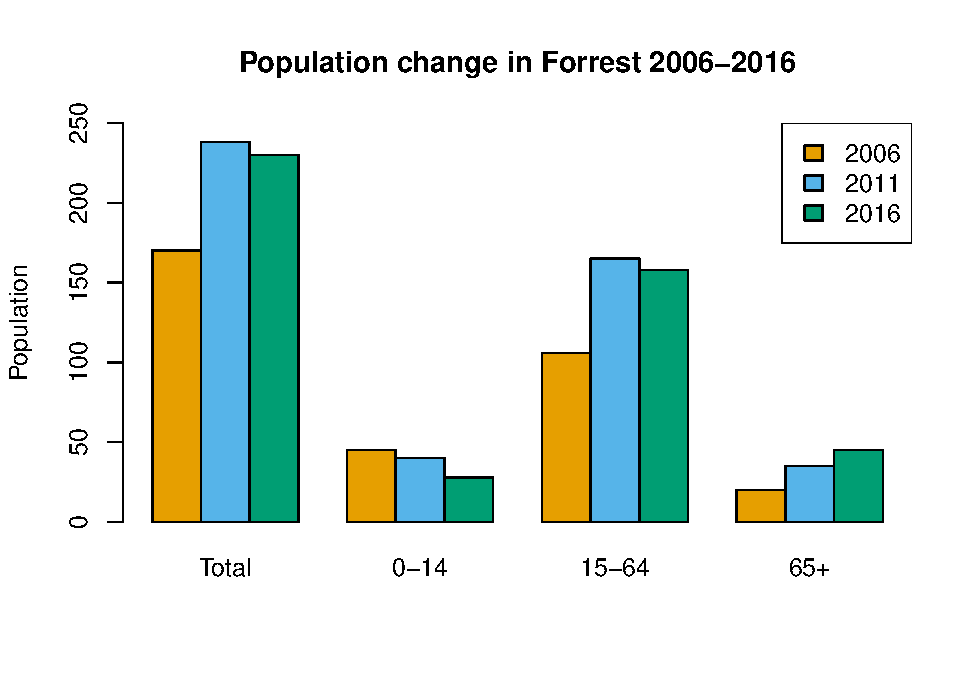
\includegraphics{Model-docs_files/figure-latex/unnamed-chunk-1-1.pdf}

\hypertarget{system-conceptualisation}{%
\section{\texorpdfstring{\emph{System conceptualisation}}{System conceptualisation}}\label{system-conceptualisation}}

The population of Forrest is not large (230 at the 2016 Census) and is easiest to split into three main cohorts: children (0-15), adults (16-64), and retirees (65+).

Each of these cohorts has a migration and death rate specific to that cohort. There are ageing (maturation) rates between the 0-14 and 15-64 cohorts.

Migration rates for each cohort are influenced by different characteristics, some of which are modelled (e.g.~job availability and housing) and some which are not but are captured within a reference (i.e.~initial) migration rate.

School enrolments are made up of local children aged 4-10 (half of the 0-14 cohort) and from `district' children (i.e., from surrounding townships that make up ``Forrest and District'').

\hypertarget{conceptual-model}{%
\subsection{Conceptual model}\label{conceptual-model}}

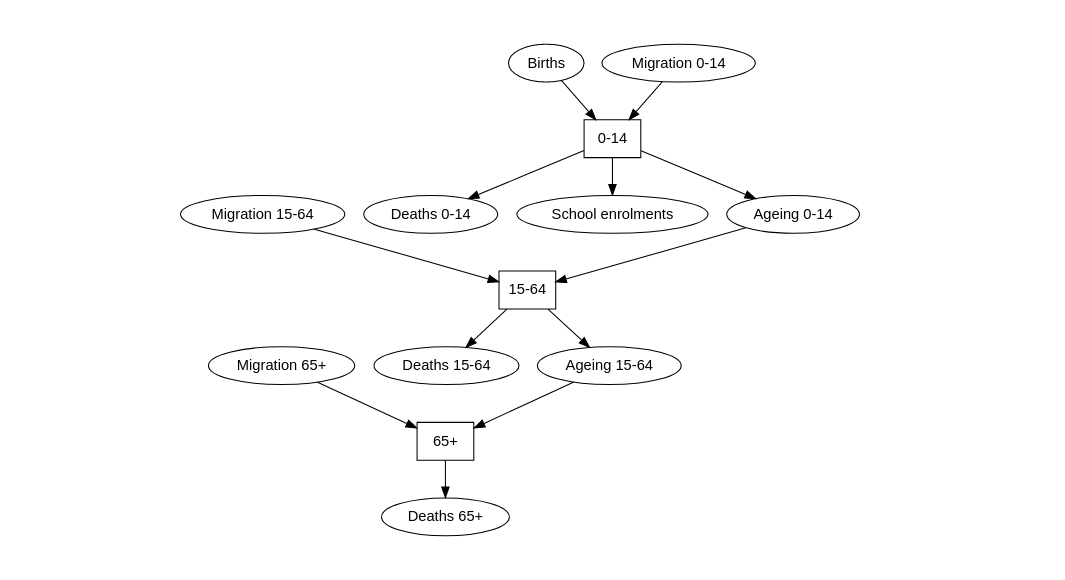
\includegraphics{Model-docs_files/figure-latex/unnamed-chunk-2-1.png}

\hypertarget{model-formulation}{%
\section{\texorpdfstring{\emph{Model formulation}}{Model formulation}}\label{model-formulation}}

The structure of this model component was based upon the model by \citet{navarro_rusem_2019}. Additional structure was added to incorporate the local school model within this component, and for the different effects on migration rate.

\hypertarget{data-sources}{%
\section{Data sources}\label{data-sources}}

\href{https://www.abs.gov.au/AUSSTATS/abs@.nsf/DetailsPage/3301.02018?OpenDocument}{Data for births.} We used data for the Colac Otway LGA.

Census data for Forrest available \href{https://www.abs.gov.au/websitedbs/D3310114.nsf/Home/2016\%20QuickStats}{here.} Data for Forrest as a distinct location is only available for 2006, 2011 and 2016 censuses.

Data for deaths was obtained from ABS.stat, which has now been decommissioned and replaced by \href{https://explore.data.abs.gov.au/}{ABS Data Explorer.} For death rates we used state-level data as this was the only way to get age-disaggregated death data.

\begin{center}\rule{0.5\linewidth}{0.5pt}\end{center}

\hypertarget{equations}{%
\section{\texorpdfstring{\emph{Equations}}{Equations}}\label{equations}}

\hypertarget{section}{%
\subsection{0-14}\label{section}}

Type: Stock\\
Formula: INTEG( Births + ``In-out migration 0-14'' - ``Ageing 0-14'' - ``Deaths 0-14''), INITIAL = 45\\
Units: people\\
Assumptions/data: Intial value from 2006 census (earliest township-specific census data available)

\hypertarget{births}{%
\subsection{Births}\label{births}}

Type: Auxiliary (rate)\\
Formula: ( ``15-64'' * fertility rate ) / 2\\
Units: people/Year\\
Assumptions/data: Number of births per year. Assume half of the 15-64 cohort are able to bear children

\hypertarget{fertility-rate}{%
\subsection{fertility rate}\label{fertility-rate}}

Type: Constant\\
Formula: 0.07\\
Units: 1/Year\\
Assumptions/data: The number of live births per woman aged 15-64 each year. Derived from calibration of the model against data.

\hypertarget{in-out-migration-0-14}{%
\subsection{In-out migration 0-14}\label{in-out-migration-0-14}}

Type: Auxiliary (rate)\\
Formula: ``migration rate 0-14'' * ``0-14''\\
Units: people/Year\\
Assumptions/data: net migration per year for 0-14 cohort

\hypertarget{migration-rate-0-14}{%
\subsection{migration rate 0-14}\label{migration-rate-0-14}}

Type: Auxiliary\\
Formula: ``migration rate 15-64'' 8 ``reference migration rate 0-14''\\
Units: 1/Year\\
Assumptions/data: Migration rate of 0-14 cohort will be strongly influenced by the migration rate of their parents' cohort.

\hypertarget{reference-migration-rate-0-14}{%
\subsection{reference migration rate 0-14}\label{reference-migration-rate-0-14}}

Type: Constant\\
Formula: -4\\
Units: Dmnl\\
Assumptions/data: Derived from calibration of the model against data.

\hypertarget{deaths-0-14}{%
\subsection{Deaths 0-14}\label{deaths-0-14}}

Type: Auxiliary (rate)\\
Formula: ``mortality rate 0-14'' * ``0-14''\\
Units: people/Year\\
Assumptions/data: Number of deaths per year of the 0-14 cohort

\hypertarget{mortality-rate-0-14}{%
\subsection{mortality rate 0-14}\label{mortality-rate-0-14}}

Type: Constant\\
Formula: 0.00031\\
Units: 1/Year\\
Assumptions/data: Derived from data aggregated at state level

\hypertarget{ageing-0-14}{%
\subsection{Ageing 0-14}\label{ageing-0-14}}

Type: Auxiliary (rate)\\
Formula: ``0-14'' / ``maturation factor 0-14''\\
Units: people/Year\\
Assumptions/data: Number of population 0-14 moving to next age group

\hypertarget{maturation-factor-0-14}{%
\subsection{maturation factor 0-14}\label{maturation-factor-0-14}}

Type: Constant\\
Formula: 14\\
Units: Year\\
Assumptions/data: The length of time a person can spend in the cohort before maturing into the next (max age - min age)

\hypertarget{section-1}{%
\subsection{15-64}\label{section-1}}

Type: Stock\\
Formula: INTEG( ``Ageing 0-14'' + ``In-out migration 15-64'' - ``Ageing 15-64'' - ``Deaths 15-64''), INITIAL = 106\\
Units: people\\
Assumptions/data: Intial value from 2006 census (earliest township-specific census data available)

\hypertarget{in-out-migration-15-64}{%
\subsection{In-out migration 15-64}\label{in-out-migration-15-64}}

Type: Auxiliary (rate)\\
Formula: ``migration rate 15-64'' * ``15-64''\\
Units: people/Year\\
Assumptions/data: Net migration per year for the 15-64 cohort

\hypertarget{migration-rate-15-64}{%
\subsection{migration rate 15-64}\label{migration-rate-15-64}}

Type: Auxiliary\\
Formula: ``reference 15-64 migration rate'' * effect of job availability on migration * effect of housing on migration * job availability unit conversion factor\\
Units: 1/Year\\
Assumptions/data: Potentially problematic if the reference rate is negative

\hypertarget{reference-15-64-migration-rate}{%
\subsection{reference 15-64 migration rate}\label{reference-15-64-migration-rate}}

Type: Constant\\
Formula: 0.011\\
Units: 1/Year\\
Assumptions/data: Migration rates calibrated against from Otway SA2 data: the average rate for 2017-2019

\hypertarget{job-availability-unit-conversion-factor}{%
\subsection{job availability unit conversion factor}\label{job-availability-unit-conversion-factor}}

Type: Constant\\
Formula: 1\\
Units: people * Year/job\\
Assumptions/data: This is a unit correction variable

\hypertarget{effect-of-job-availability-on-migration}{%
\subsection{effect of job availability on migration}\label{effect-of-job-availability-on-migration}}

Type: Auxiliary\\
Formula: (``job vacancies (agriculture) filled externally''+``job vacancies (other) filled externally''+``job vacancies (tourism) filled externally'') / ``working-age population''\\
Units: job/(people * Year)\\
Assumptions/data: The job to labour force ratio

\hypertarget{effect-of-housing-on-migration}{%
\subsection{effect of housing on migration}\label{effect-of-housing-on-migration}}

Type: Auxiliary\\
Formula: IF THEN ELSE( housing supply demand ratio \textgreater{} 1,
(IF THEN ELSE(``social housing supply/demand ratio'' = 0,
(average house price/reference average house price) * housing supply demand ratio,
(average house price/reference average house price) * housing supply demand ratio * ``social housing supply/demand ratio'')), 1)\\
Units: Dmnl\\
Assumptions/data: As demand goes up, supply goes down and the ratio also goes down, and the prices go up.
Additionally, if the housing supply/demand ratio is less than 1, then there aren't enough houses available for new families to move in unless existing families move out, so the effect of housing on net migration is zero (this also affects all other effect variables on migration).

\hypertarget{deaths-15-64}{%
\subsection{Deaths 15-64}\label{deaths-15-64}}

Type: Auxiliary (rate)\\
Formula: ``15-64'' * ``mortality rate 15-64''\\
Units: people/Year\\
Assumptions/data: Number of deaths in a year for the 15-64 cohort

\hypertarget{mortality-rate-15-64}{%
\subsection{mortality rate 15-64}\label{mortality-rate-15-64}}

Type: Constant\\
Formula: 0.00156\\
Units: 1/Year\\
Assumptions/data: Constant derived from data aggregated at state level

\hypertarget{ageing-15-64}{%
\subsection{Ageing 15-64}\label{ageing-15-64}}

Type: Auxiliary (rate)\\
Formula: ``15-64'' / ``maturation factor 15-64''\\
Units: people/Year\\
Assumptions/data: Number of population 15-64 moving to next age group

\hypertarget{maturation-factor-15-64}{%
\subsection{maturation factor 15-64}\label{maturation-factor-15-64}}

Type: Constant\\
Formula: 49\\
Units: Year\\
Assumptions/data: Cohort residence time max age - min age

\hypertarget{section-2}{%
\subsection{65+}\label{section-2}}

Type: Stock\\
Formula: INTEG( ``Ageing 15-64'' + ``In-out migration 65+'' - ``Deaths 65+''), INITAL = 20\\
Units: people\\
Assumptions/data: Inital value taken from 2006 Census data (earliest township-specific census data available)

\hypertarget{deaths-65}{%
\subsection{Deaths 65+}\label{deaths-65}}

Type: Auxiliary (rate)\\
Formula: ``65+'' * ``mortality rate 65+''\\
Units: people/Year\\
Assumptions/data:

\hypertarget{mortality-rate-65}{%
\subsection{mortality rate 65+}\label{mortality-rate-65}}

Type: Constant\\
Formula: 0.03694\\
Units: 1/Year\\
Assumptions/data: Derived from data aggregated at state level

\hypertarget{in-out-migration-65}{%
\subsection{In-out migration 65+}\label{in-out-migration-65}}

Type: Auxiliary (rate)\\
Formula: ``migration rate 65+'' * ``65+''\\
Units: people/Year\\
Assumptions/data: Net migration per year

\hypertarget{migration-rate-65}{%
\subsection{migration rate 65+}\label{migration-rate-65}}

Type: Auxiliary\\
Formula: ``reference 65+ migration rate'' * effect of housing on migration\\
Units: 1/Year\\
Assumptions/data:

\hypertarget{reference-migration-rate-65}{%
\subsection{reference migration rate 65+}\label{reference-migration-rate-65}}

Type: Constant\\
Formula: -0.022\\
Units: 1/Year\\
Assumptions/data: Derived from calibration of the model against data.

\hypertarget{total-population}{%
\subsection{total population}\label{total-population}}

Type: Auxiliary\\
Formula: ``0-14'' + ``15-64'' + ``65+''\\
Units: people\\
Assumptions/data: sum of all population cohorts

\hypertarget{school-enrolments}{%
\subsection{School Enrolments}\label{school-enrolments}}

Type: Stock\\
Formula: INTEG(New enrolments - Outgoing school cohort), INITIAL = 31\\
Units: people\\
Assumptions/data: Inital data 31 students enrolled in 2019

\hypertarget{new-enrolments}{%
\subsection{New enrolments}\label{new-enrolments}}

Type: Auxiliary (rate)\\
Formula: (( district 0 to 14 cohort + ``0-14'' )/cohort time * enrolment ratio)\\
Units: people/Year\\
Assumptions/data: To prevent `re-enrolment' of the same student each year, divide the cohort values by `cohort time' so each enrolment is new.

\hypertarget{cohort-time}{%
\subsection{cohort time}\label{cohort-time}}

Type: Constant\\
Formula: 7\\
Units: Dmnl\\
Assumptions/data: To prevent `re-enrolment' of the same student each year, divide the cohort values by 7 so each enrolment is new.

\hypertarget{enrolment-ratio}{%
\subsection{enrolment ratio}\label{enrolment-ratio}}

Type: Constant\\
Formula: 0.5\\
Units: 1/Year\\
Assumptions/data: Only half of the 0-14 cohort will enrol at the local primary school (age 4-10)

\hypertarget{district-0-14-cohort}{%
\subsection{district 0-14 cohort}\label{district-0-14-cohort}}

Type: Auxiliary\\
Formula: INTEGER (RANDOM NORMAL ( 0, 76, 38, 1, 0 ))\\
Units: people\\
Assumptions/data: Selecting from a normal distrbution to obtain values for enrolments external to Forrest's population. The parameters are min = 0, max = 76, mean = 38, SD = 1, based on populations from the townships in the district.

\hypertarget{number-of-childcare-enrolments}{%
\subsection{number of childcare enrolments}\label{number-of-childcare-enrolments}}

Type: Auxiliary\\
Formula: INTEGER ( ( district 0 to 14 cohort + ``0-14'' ) * 0.25)\\
Units: people\\
Assumptions/data: Arbitrary value of one quarter of 0-14 cohort (have no data for this)

\hypertarget{district-kids-parents-cohort}{%
\subsection{district kids' parents cohort}\label{district-kids-parents-cohort}}

Type: Auxiliary\\
Formula: INTEGER ( (district 0 to 14 cohort * 0.75) * 1.5)\\
Units: people\\
Assumptions/data: Multiply by 1.5 to capture both parents with some wiggle room for single parents etc
Multiply by 0.75 to take into account 0.5 enrolment ratio (ie, only half of cohort are of primary school age) and 0.25 for childcare

\hypertarget{outgoing-school-cohort}{%
\subsection{Outgoing school cohort}\label{outgoing-school-cohort}}

Type: Auxiliary (rate)\\
Formula: School Enrolments / maturation of school students\\
Units: people/Year\\
Assumptions/data:

\hypertarget{maturation-of-school-students}{%
\subsection{maturation of school students}\label{maturation-of-school-students}}

Type: Constant\\
Formula: 7\\
Units: people\\
Assumptions/data: School age cohort tenure time (max age - min age)

\hypertarget{land-use-component}{%
\chapter{Land Use component}\label{land-use-component}}

There are four major types of land use in Forrest: Agriculture (incorporating crop farming and livestock farming), Housing, Forest, and Protected (national park). As an initial condition, we assume that agricultural land which is \textgreater40 hectares in size is classified as Farming Zone, and is thus protected from land use change (although the Forrest community would like this zoning modified so that Farming Zone land within the township could have more than one residence built on it). Housing land is primarily within the township. \href{https://www.planning.vic.gov.au/__data/assets/pdf_file/0027/97182/PPN42-Applying-the-Rural-Zones_June-2015.pdf}{This link} discusses the different rural planning zones.

\hypertarget{problem-definition-1}{%
\section{\texorpdfstring{\emph{Problem definition}}{Problem definition}}\label{problem-definition-1}}

\begin{enumerate}
\def\labelenumi{\arabic{enumi}.}
\tightlist
\item
  Agricultural land fertility is a driver of agricultural business profits. In general, the world needs to use less additional fertilisers to improve the health of ecosystems. Forrest is a hub for regenerative agriculture -- where the land is improved as a result of agriculture, rather than stripped of nutrients as in traditional farming.
\end{enumerate}

\emph{Dynamic hypothesis:}
Regenerative agriculture limits the use of fertilisers, which reduces agricultural runoff into waterways, improving local water quality and the environment generally. It also boosts agricultural profits.

\begin{enumerate}
\def\labelenumi{\arabic{enumi}.}
\setcounter{enumi}{1}
\tightlist
\item
  There is not currently a great deal of land use change in Forrest. Agricultural businesses and housing demand are the greatest pressures on land use.
\end{enumerate}

\emph{Dynamic hypothesis:}
Residents have suggested petitioning Council to change the laws restricting multiple buildings on agricultural land (the `40ha' rule), which may increase land transfer between ag and housing, and an increase in agricultural business may increase land transfer between bush and agriculture.

\hypertarget{system-conceptualisation-1}{%
\section{\texorpdfstring{\emph{System conceptualisation}}{System conceptualisation}}\label{system-conceptualisation-1}}

The stock of land in Forrest is fixed (approx 12,000 hectares). We assume four land use types - Agriculture, Forest, Housing and Protected. Protected land can only be increased from Forest land, and once it is there it remains there. Housing can be increased from Agriculture or Farming but once land is Housing land, it remains there. Agriculture and Forest land can cycle between the two.

Housing land has pressures from housing demand. Agriculture land has pressure from agricultural businesses.

Fertilisation intensity and consumption does not affect the rest of the model.

\hypertarget{conceptual-model-1}{%
\subsection{Conceptual model}\label{conceptual-model-1}}

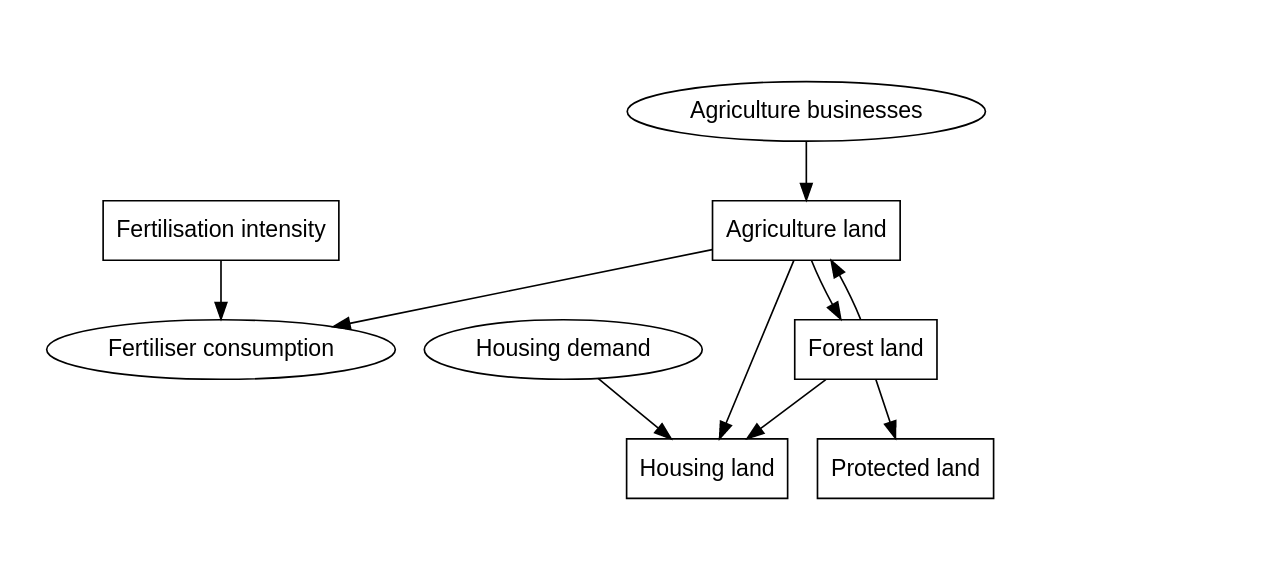
\includegraphics{Model-docs_files/figure-latex/unnamed-chunk-3-1.png}

\hypertarget{model-formulation-1}{%
\section{\texorpdfstring{\emph{Model formulation}}{Model formulation}}\label{model-formulation-1}}

The land use component was inspired by the FeliX model \citet{rydzak_felix3_2013}. There are four stocks, one for each of the land use types, and a small structure to model fertiliser consumption. Another small structure is present to set maximum values for each land use stock. Each transfer rate between land stocks is affected by two variables: a `change' variable (FeliX characterises this as a value which measures the `need' for change between land use types, so we represent this as a pressure for change); and an `allocation time' variable, which represents the amount of time it takes to change from one land use to another.

\hypertarget{data-sources-1}{%
\section{Data sources}\label{data-sources-1}}

Data and code are available at \url{https://github.com/pelagikat/Local-SDGs-systems-model}

Land use data was obtained from the \href{http://vro.agriculture.vic.gov.au/dpi/vro/vrosite.nsf/pages/vluis}{Victorian Land Use Information System (VLUIS)}. This is a series of seven spatial datasets with land use classes which we clipped to the extent of the Forrest township. The land use classes were categorised into the model variables as follows:

Housing:\\
Detached Home\\
Residential Rural / Rural Lifestyle (0.4 to 20 Ha)\\
Vacant Residential Home Site / Surveyed Lot\\
Vacant Residential Rural / Rural Lifestyle (0.4 to 20ha)

Forest:\\
Creek Reserve (Fresh Water)\\
Forest Reserves - Public\\
Reserved Land\\
Softwood Plantation\\
Nature Reserve Area
Water Supply\\
Unclassified Private Land\\
Native Hardwood (standing timber)

Agriculture:\\
Mixed farming and grazing (generally more than 20ha)\\
Livestock Production (Dairy Cattle)\\
Livestock Production (Beef Cattle)\\
Market Garden - Vegetables (generally less than 20ha plantings)

Protected:\\
National Park - Land\\
Conservation Area - Public

\begin{center}\rule{0.5\linewidth}{0.5pt}\end{center}

\hypertarget{equations-1}{%
\section{\texorpdfstring{\emph{Equations}}{Equations}}\label{equations-1}}

\hypertarget{agricultural-to-housing-transfer-rate}{%
\subsection{Agricultural to Housing transfer rate}\label{agricultural-to-housing-transfer-rate}}

Type: Rate\\
Formula: MAX(0, MIN (max land housing, agriculture to housing change * ( Agriculture Land - agriculture protected land ) / agriculture to housing land allocation time ))\\
Units: ha/Year\\
Assumptions: The amount of agriculture land will not drop below the value of the agriculture protected land variable

\hypertarget{agriculture-land}{%
\subsection{Agriculture Land}\label{agriculture-land}}

Type: Stock\\
Formula: INTEG (Forest to Agriculture transfer rate - Agricultural to Housing transfer rate -
Agriculture to Forest transfer rate), INITIAL = INIT agricultural land\\
Units: hectare\\
Assumptions:

\hypertarget{agriculture-protected-land}{%
\subsection{agriculture protected land}\label{agriculture-protected-land}}

Type: Constant\\
Formula: 1533.8\\
Units: hectare\\
Assumptions: LU 2008 data: all farming and livestock land use \textgreater40ha as equivalent to Farming Zone \href{https://www.planning.vic.gov.au/__data/assets/pdf_file/0027/97182/PPN42-Applying-the-Rural-Zones_June-2015.pdf}{(see here)}

\hypertarget{agriculture-to-forest-change}{%
\subsection{agriculture to forest change}\label{agriculture-to-forest-change}}

Type: Auxiliary\\
Formula: (``number of businesses (agriculture)'' * average land per agricultural business) / Agriculture Land\\
Units: Dmnl\\
Assumptions:

\hypertarget{agriculture-to-forest-land-allocation-time}{%
\subsection{agriculture to forest land allocation time}\label{agriculture-to-forest-land-allocation-time}}

Type: Constant\\
Formula: 2.5\\
Units: Year\\
Assumptions: Calibrated against data

\hypertarget{agriculture-to-forest-transfer-rate}{%
\subsection{Agriculture to Forest transfer rate}\label{agriculture-to-forest-transfer-rate}}

Type: Rate\\
Formula: MAX(0, MIN ( max land forest, agriculture to forest change * ( Agriculture Land - agriculture protected land) / agriculture to forest land allocation time ))\\
Units: ha/Year\\
Assumptions:

\hypertarget{agriculture-to-housing-change}{%
\subsection{agriculture to housing change}\label{agriculture-to-housing-change}}

Type: Auxiliary\\
Formula: (average land per house * housing demand) / Housing Land\\
Units: Dmnl\\
Assumptions:

\hypertarget{agriculture-to-housing-land-allocation-time}{%
\subsection{agriculture to housing land allocation time}\label{agriculture-to-housing-land-allocation-time}}

Type: Constant\\
Formula: 500\\
Units: Year\\
Assumptions: Calibrated against data

\hypertarget{average-land-per-agricultural-business}{%
\subsection{average land per agricultural business}\label{average-land-per-agricultural-business}}

Type: Constant\\
Formula: 17.3\\
Units: hectare/structure\\
Assumptions: Value derived from Land Use spatial dataset

\hypertarget{average-land-per-house}{%
\subsection{average land per house}\label{average-land-per-house}}

Type: Auxiliary\\
Formula: (land per house LDRZ + land per house RLZ) / 2\\
Units: hectares/structure\\
Assumptions: Mean value of Low Density Residential Zone and Rural Living Zone

\hypertarget{fertilisation-intensity}{%
\subsection{Fertilisation Intensity}\label{fertilisation-intensity}}

Type: Stock\\
Formula: INTEG ( Fertilisation intensity change rate), INITIAL = INIT Fertilisation Intensity\\
Units: TonNutrient/(ha*Year)\\
Assumptions: Intensity of fertilisation practices per ha per year.

\hypertarget{fertilisation-intensity-change}{%
\subsection{fertilisation intensity change}\label{fertilisation-intensity-change}}

Type: Constant\\
Formula: -0.1\\
Units: Dmnl\\
Assumptions: Calibrated against data

\hypertarget{fertilisation-intensity-change-rate}{%
\subsection{Fertilisation intensity change rate}\label{fertilisation-intensity-change-rate}}

Type: Stock\\
Formula: Fertilisation Intensity * fertilisation intensity change / time to adjust fertilisation intensity\\
Units: TonNutrient/(Year * Year * ha)\\
Assumptions:

\hypertarget{fertiliser-consumption}{%
\subsection{fertiliser consumption}\label{fertiliser-consumption}}

Type: Auxiliary\\
Formula: ( Fertilisation Intensity * Agriculture Land )\\
Units: TonNutrient/Year\\
Assumptions:

\hypertarget{forest-land}{%
\subsection{Forest Land}\label{forest-land}}

Type: Stock\\
Formula: INTEG (Agriculture to Forest transfer rate - Forest to Agriculture transfer rate - Forest to Housing transfer rate - Forest to Protected transfer rate), INITIAL = INIT forest land\\
Units: hectare\\
Assumptions:

\hypertarget{forest-to-agriculture-change}{%
\subsection{forest to agriculture change}\label{forest-to-agriculture-change}}

Type: Constant\\
Formula: 0.4\\
Units: Dmnl\\
Assumptions: Calibrated against data

\hypertarget{forest-to-agriculture-land-allocation-time}{%
\subsection{forest to agriculture land allocation time}\label{forest-to-agriculture-land-allocation-time}}

Type: Constant\\
Formula: 19\\
Units: Year\\
Assumptions: Calibrated against data

\hypertarget{forest-to-agriculture-transfer-rate}{%
\subsection{Forest to Agriculture transfer rate}\label{forest-to-agriculture-transfer-rate}}

Type: Auxiliary\\
Formula: MAX ( 0, MIN ( max land ag, forest to agriculture change * ( Forest Land ) / ( forest to agriculture land allocation time ) ))\\
Units: ha/Year\\
Assumptions:

\hypertarget{forest-to-housing-change}{%
\subsection{forest to housing change}\label{forest-to-housing-change}}

Type: Auxiliary\\
Formula: (average land per house * housing demand ) / Housing Land\\
Units: Dmnl\\
Assumptions:

\hypertarget{forest-to-housing-land-allocation-time}{%
\subsection{forest to housing land allocation time}\label{forest-to-housing-land-allocation-time}}

Type: Constant\\
Formula: 500\\
Units: Year\\
Assumptions: Calibrated against data

\hypertarget{forest-to-housing-transfer-rate}{%
\subsection{Forest to Housing transfer rate}\label{forest-to-housing-transfer-rate}}

Type: Auxiliary\\
Formula: MAX(0, MIN ( max land housing, forest to housing change * ( Forest Land ) / forest to housing land allocation time ))\\
Units: ha/Year\\
Assumptions:

\hypertarget{forest-to-protected-allocation-time}{%
\subsection{forest to protected allocation time}\label{forest-to-protected-allocation-time}}

Type: Constant\\
Formula: 542\\
Units: Year\\
Assumptions: Calibrated against data

\hypertarget{forest-to-protected-change}{%
\subsection{forest to protected change}\label{forest-to-protected-change}}

Type: Constant\\
Formula: 25\\
Units: Dmnl\\
Assumptions: Calibrated against data

\hypertarget{forest-to-protected-transfer-rate}{%
\subsection{Forest to Protected transfer rate}\label{forest-to-protected-transfer-rate}}

Type: Auxiliary\\
Formula: MAX(0, MIN ( max land protected, forest to protected change * ( Forest Land / forest to protected allocation time )))\\
Units: hectare/Year\\
Assumptions:

\hypertarget{housing-land}{%
\subsection{Housing Land}\label{housing-land}}

Type: Stock\\
Formula: INTEG( Agricultural to Housing transfer rate + Forest to Housing transfer rate), INITIAL = INIT housing land\\
Units: hectare\\
Assumptions:

\hypertarget{init-agricultural-land}{%
\subsection{INIT agricultural land}\label{init-agricultural-land}}

Type: Constant\\
Formula: 3549.5\\
Units: hectare\\
Assumptions: Land area in year 2006 (earliest data available).

\hypertarget{init-fertilisation-intensity}{%
\subsubsection{INIT Fertilisation Intensity}\label{init-fertilisation-intensity}}

Type: Constant\\
Formula: 0.254\\
Units: TonNutrient/(ha*Year)\\
Assumptions: In 2008, farming in Cogangamite used 0.254 tons/ha/year

\hypertarget{init-forest-land}{%
\subsection{INIT forest land}\label{init-forest-land}}

Type: Constant\\
Formula: 4436\\
Units: hectare\\
Assumptions: Land area in year 2008 (earliest data available).

\hypertarget{init-housing-land}{%
\subsection{INIT housing land}\label{init-housing-land}}

Type: Constant\\
Formula: 57.3\\
Units: hectare\\
Assumptions: Land area in year 2008 (earliest data available).

\hypertarget{init-protected-land}{%
\subsection{INIT protected land}\label{init-protected-land}}

Type: Constant\\
Formula: 1283.7\\
Units: hectare\\
Assumptions: Land area in year 2006 (earliest data available).

\hypertarget{land-per-house-ldrz}{%
\subsection{land per house LDRZ}\label{land-per-house-ldrz}}

Type: Constant\\
Formula: 0.82\\
Units: hectares/structure\\
Assumptions: Low Density Residential Zone with a lot size of a minimum of 0.4 ha in areas with no reticulated sewerage. \href{https://www.planning.vic.gov.au/__data/assets/pdf_file/0026/97172/PPN37-Rural-Residential-Development_June-2015.pdf}{See here}. Mean value of LDRZ lot size is 0.82 hectares

\hypertarget{land-per-house-rlz}{%
\subsection{land per house RLZ}\label{land-per-house-rlz}}

Type: Constant\\
Formula: 7.3\\
Units: hectares/structure\\
Assumptions: Rural Living Zone specifies a lot size of at least 2 hectares and provides opportunities for some rural uses to occur. \href{https://www.planning.vic.gov.au/__data/assets/pdf_file/0026/97172/PPN37-Rural-Residential-Development_June-2015.pdf}{See here}. Mean value of RLZ lot size is 7.3 hectares

\hypertarget{max-land}{%
\subsection{max land}\label{max-land}}

Type: Constant\\
Formula: 12041\\
Units: hectares/Year\\
Assumptions: Limiting factor for land stock expansion

\hypertarget{max-land-ag}{%
\subsection{max land ag}\label{max-land-ag}}

Type: Auxiliary\\
Formula: max land-Forest Land-Housing Land-Protected Land\\
Units: hectares\\
Assumptions:

\hypertarget{max-land-forest}{%
\subsection{max land forest}\label{max-land-forest}}

Type: Auxiliary\\
Formula: max land-Agriculture Land-Housing Land-Protected Land\\
Units: hectares\\
Assumptions:

\hypertarget{max-land-housing}{%
\subsection{max land housing}\label{max-land-housing}}

Type: Auxiliary\\
Formula: max land-Agriculture Land-Forest Land-Protected Land\\
Units: hectares\\
Assumptions:

\hypertarget{max-land-protected}{%
\subsection{max land protected}\label{max-land-protected}}

Type: Auxiliary\\
Formula: max land-Agriculture Land-Forest Land-Housing Land\\
Units: hectares\\
Assumptions:

\hypertarget{protected-land}{%
\subsection{Protected Land}\label{protected-land}}

Type: Stock\\
Formula: INTEG (Forest to Protected transfer rate), INITIAL = INIT protected land\\
Units: hectare\\
Assumptions:

\hypertarget{time-to-adjust-fertilisation-intensity}{%
\subsection{time to adjust fertilisation intensity}\label{time-to-adjust-fertilisation-intensity}}

Type: Constant\\
Formula: 4\\
Units: Year\\
Assumptions: Calibrated against data

\hypertarget{total-land}{%
\subsection{total land}\label{total-land}}

Type: Auxiliary\\
Formula: Agriculture Land + Forest Land + Housing Land + Protected Land\\
Units: hectares\\
Assumptions: Mean total land area 2008-2017 = 12427 hectares

\hypertarget{housing-component}{%
\chapter{Housing component}\label{housing-component}}

There are multiple intertwined issues to do with housing in Forrest. Supply cannot meet demand; tourism is reducing the available residential housing stock; development is hamstrung by existing waste management requirements. The supply issue is driving up house prices, and residents on lower incomes are being driven out because of cost.

\hypertarget{problem-definition-2}{%
\section{\texorpdfstring{\emph{Problem definition}}{Problem definition}}\label{problem-definition-2}}

\begin{enumerate}
\def\labelenumi{\arabic{enumi}.}
\tightlist
\item
  Colac Otway Shire have designated that Forrest remain a low growth community and estimated a release of 3.5 permits per year for residential land development. There has only been one permit issued per year since 2011, so development has been below expected levels. There is scope for greater development in the future.
\end{enumerate}

\emph{Dynamic hypothesis:}
Building permits are not being granted by Council because potential developments cannot meet septic tank regulations. New wastewater infrastructure is required before any significant development may occur.

\begin{enumerate}
\def\labelenumi{\arabic{enumi}.}
\setcounter{enumi}{1}
\tightlist
\item
  Cost and availability of housing is an issue. Tourism businesses purchase properties for accommodation, removing them from the pool of available residential housing. This in turn drives up prices due to scarcity of supply. Other potential new residents also struggle to find housing, and anecdotally must wait until existing residents move away or travel.
\end{enumerate}

\emph{Dynamic hypothesis:}
Lack of housing development due to wastewater issues is constraining the housing and tourism accommodation supply.

\begin{enumerate}
\def\labelenumi{\arabic{enumi}.}
\setcounter{enumi}{2}
\tightlist
\item
  Median house prices have increased 188\% since 2009, while median rents have increased by 30\%. This puts a number of residents into mortgage or rent stress.
\end{enumerate}

\emph{Dynamic hypothesis:}
House prices are artificially high in much of Victoria (property market bubble), and the housing supply issue additionally inflates prices. Social housing (hypothetical) may relieve rent stress.

\hypertarget{system-conceptualisation-and-formulation}{%
\section{\texorpdfstring{\emph{System conceptualisation and formulation}}{System conceptualisation and formulation}}\label{system-conceptualisation-and-formulation}}

There are two uses for housing in Forrest; residential and tourism. The central housing stock structure is built with Housing Supply, which has construction and demolition as flows. The Housing Supply stock drains into Tourism Housing and Residential Housing stocks. Housing demand is influenced by total population and Number of Tourists. Separate from this structure is the Social Housing Supply structure, which is a scenario variable and not active in the BAU scenario as there is currently no social housing in Forrest.

Leading off the Residential Housing stock is the housing stress structures, split into mortgage stress and rent stress, defined as when housing costs (rent or mortgage payments) exceed 30\% of household income. The income and housing costs were split into three levels; low, medium and high.

\hypertarget{conceptual-model-2}{%
\subsection{Conceptual model}\label{conceptual-model-2}}

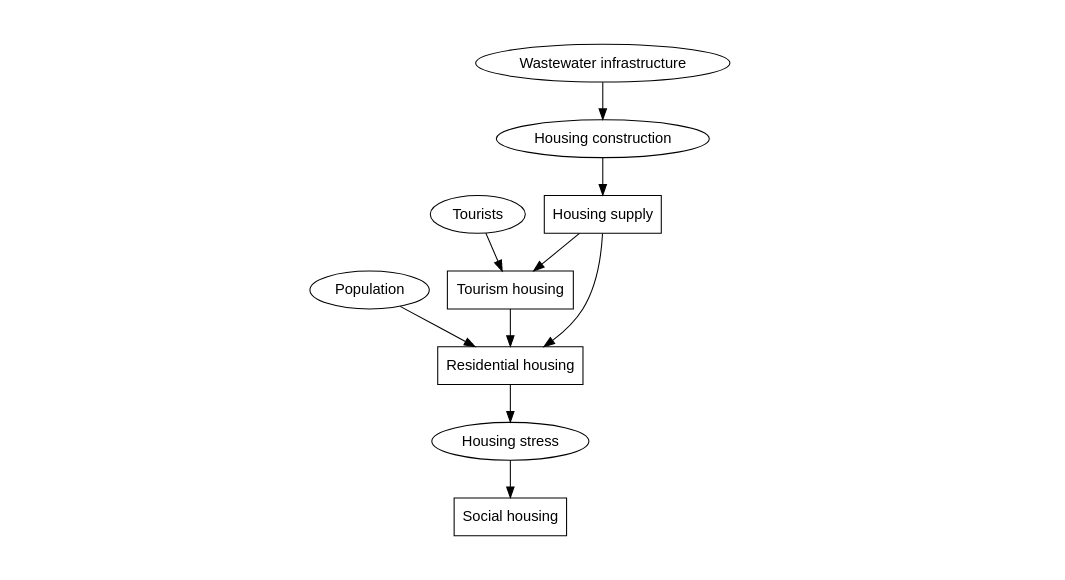
\includegraphics{Model-docs_files/figure-latex/unnamed-chunk-4-1.png}

\hypertarget{data-sources-2}{%
\section{Data sources}\label{data-sources-2}}

Data is available at \url{https://github.com/pelagikat/Local-SDGs-systems-model}

Data was obtained from \href{https://www.abs.gov.au/websitedbs/censushome.nsf/home/tablebuilder}{ABS Table Builder} for housing tenure, \href{http://vro.agriculture.vic.gov.au/dpi/vro/vrosite.nsf/pages/vluis}{Victorian Land Use Information System (VLUIS)} for numbers of properties, and \href{https://www.aupropertyreport.com/suburb-report/forrest-3236-vic/}{Aus Property Report} for house sale and rental prices.

\begin{center}\rule{0.5\linewidth}{0.5pt}\end{center}

\hypertarget{equations-2}{%
\section{\texorpdfstring{\emph{Equations}}{Equations}}\label{equations-2}}

\hypertarget{percent}{%
\subsection{``30 percent''}\label{percent}}

Type: Constant\\
Formula: 0.3\\
Units: fraction\\
Assumptions: Housing stress is defined as housing costs that exceed 30\% of household income.

\hypertarget{annual-mortgage-cost-by-income-grouplow-income}{%
\subsection{Annual Mortgage Cost By Income Group{[}low income{]}}\label{annual-mortgage-cost-by-income-grouplow-income}}

Type: Stock\\
Formula: INTEG (Mortgage rate change{[}low income{]}), INITIAL = 16176\\
Units: dollars\\
Assumptions: Initial value 2017 loan repayment value annualised (see data in Github)

\hypertarget{annual-mortgage-cost-by-income-groupmid-income}{%
\subsection{Annual Mortgage Cost By Income Group{[}mid income{]}}\label{annual-mortgage-cost-by-income-groupmid-income}}

Type: Stock\\
Formula: INTEG (Mortgage rate change{[}mid income{]}), INITIAL = 18876)\\
Units: dollars\\
Assumptions: Initial value 2017 loan repayment value annualised (see data in Github)

\hypertarget{annual-mortgage-cost-by-income-grouphigh-income}{%
\subsection{Annual Mortgage Cost By Income Group{[}high income{]}}\label{annual-mortgage-cost-by-income-grouphigh-income}}

Type: Stock\\
Formula: INTEG (Mortgage rate change{[}high income{]}), INITIAL = 48288\\
Units: dollars\\
Assumptions: Initial value 2017 loan repayment value annualised (see data in Github)

\hypertarget{annual-rent-cost-by-income-grouplow-income}{%
\subsection{Annual Rent Cost By Income Group{[}low income{]}}\label{annual-rent-cost-by-income-grouplow-income}}

Type: Stock\\
Formula: INTEG (Rent rate change{[}low income{]}), INITIAL = 11964\\
Units: dollars\\
Assumptions: Initial value 2017 rent payment value annualised (see data in Github)

\hypertarget{annual-rent-cost-by-income-groupmid-income}{%
\subsection{Annual Rent Cost By Income Group{[}mid income{]}}\label{annual-rent-cost-by-income-groupmid-income}}

Type: Stock\\
Formula: INTEG (Rent rate change{[}mid income{]}), INITIAL = 13524\\
Units: dollars\\
Assumptions: Initial value 2017 rent payment value annualised (see data in Github)

\hypertarget{annual-rent-cost-by-income-grouphigh-income}{%
\subsection{Annual Rent Cost By Income Group{[}high income{]}}\label{annual-rent-cost-by-income-grouphigh-income}}

Type: Stock\\
Formula: = INTEG (Rent rate change{[}high income{]}), INITIAL = 13776\\
Units: dollar\\
Assumptions: Initial value 2017 rent payment value annualised (see data in Github)

\hypertarget{average-house-price}{%
\subsection{average house price}\label{average-house-price}}

Type: Auxiliary\\
Formula: effect of supply demand ratio on house prices * reference average house price\\
Units: dollars\\
Assumptions:

\hypertarget{average-size-of-household}{%
\subsection{average size of household}\label{average-size-of-household}}

Type: Constant\\
Formula: 2\\
Units: people/structure\\
Assumptions: From ABS census data (consistent for 2011 and 2016)

\hypertarget{consumer-price-index}{%
\subsection{consumer price index}\label{consumer-price-index}}

Type: Constant\\
Formula: 1.009\\
Units: Dmnl\\
Assumptions: CPI is the standard Australian inflationary measure. CPI rose 0.9\% in 2020, data from \href{https://www.abs.gov.au/statistics/economy/price-indexes-and-inflation/consumer-price-index-australia/latest-release\#data-download}{Australian Bureau of Statistics.}

\hypertarget{current-time}{%
\subsection{Current time}\label{current-time}}

Type: Constant\\
Formula: 2021\\
Units: Year\\
Assumptions: This variable is present to induce a delay to the model run year (2021).

\hypertarget{effect-of-supply-demand-ratio-on-house-prices}{%
\subsection{effect of supply demand ratio on house prices}\label{effect-of-supply-demand-ratio-on-house-prices}}

Type: Auxiliary\\
Formula: table for effect of supply demand ratio on house prices ( housing supply demand ratio )\\
Units: Dmnl\\
Assumptions: Idea derived from \citet{ozbas_modeling_2014}

\hypertarget{fraction-of-mortgaged-houses}{%
\subsection{fraction of mortgaged houses}\label{fraction-of-mortgaged-houses}}

Type: Constant\\
Formula: 0.19\\
Units: fraction\\
Assumptions: From ABS Census data (see data in Github)

\hypertarget{fraction-of-rented-houses}{%
\subsection{fraction of rented houses}\label{fraction-of-rented-houses}}

Type: Constant\\
Formula: 0.09\\
Units: fraction\\
Assumptions: From ABS Census data (see data in Github)

\hypertarget{housing-build-delay}{%
\subsection{housing build delay}\label{housing-build-delay}}

Type: Constant\\
Formula: 2\\
Units: Year\\
Assumptions: it takes 2 years from approval to build completion

\hypertarget{housing-construction}{%
\subsection{Housing construction}\label{housing-construction}}

Type: Auxiliary\\
Formula: IF THEN ELSE ( Wastewater availability \textgreater{} 0 :AND: Housing Land \textgreater{} housing land occupied, housing discrepancy delay, 0)\\
Units: structure/Year\\
Assumptions: New construction will not occur until wastewater infrastructure has been built. Additionally, the amount of housing land must be greater than the amount of land occupied already by houses.

\hypertarget{housing-demand}{%
\subsection{housing demand}\label{housing-demand}}

Type: Auxiliary\\
Formula: (number of desired residential households + number of desired tourist houses)\\
Units: structure\\
Assumptions:

\hypertarget{housing-demolition}{%
\subsection{Housing demolition}\label{housing-demolition}}

Type: Auxiliary\\
Formula: housing demolition rate * Housing Supply\\
Units: structure/Year\\
Assumptions:

\hypertarget{housing-demolition-rate}{%
\subsection{housing demolition rate}\label{housing-demolition-rate}}

Type: Constant\\
Formula: 0\\
Units: fraction/Year\\
Assumptions: For a BAU scenario, no houses are being constructed or demolished.

\hypertarget{housing-discrepancy}{%
\subsection{housing discrepancy}\label{housing-discrepancy}}

Type: Auxiliary\\
Formula: MIN(housing demand-(Residential Housing + Tourism Housing + Social Housing Supply), 140)\\
Units: structure\\
Assumptions: The formula assumes the number of houses will not go below the number recorded in the 2016 census (140)

\hypertarget{housing-discrepancy-delay}{%
\subsection{housing discrepancy delay}\label{housing-discrepancy-delay}}

Type: Auxiliary\\
Formula: -(DELAY3(housing discrepancy/housing transfer delay, housing build delay + Current time ))\\
Units: structure/Year\\
Assumptions: This variable introduces a delay between the housing discrepancy occurring and the construction occurring in response.

\hypertarget{housing-land-occupied}{%
\subsection{housing land occupied}\label{housing-land-occupied}}

Type: Auxiliary\\
Formula: minimum average land per house * (Residential Housing + Tourism Housing + Social Housing Supply)\\
Units: hectares\\
Assumptions: Housing will not achieve a density less than \emph{minimum average land per house}

\hypertarget{housing-supply}{%
\subsection{Housing Supply}\label{housing-supply}}

Type: Stock\\
Formula: INTEG (Housing construction - Housing demolition - Residential housing allocation rate - Tourism housing allocation rate), INITIAL = 100)\\
Units: structure\\
Assumptions: Initial value from 2006 census data

\hypertarget{housing-supply-demand-ratio}{%
\subsection{housing supply demand ratio}\label{housing-supply-demand-ratio}}

Type: Auxiliary\\
Formula: (Residential Housing + Tourism Housing + Social Housing Supply) / housing demand\\
Units: Dmnl\\
Assumptions:

\hypertarget{housing-transfer-delay}{%
\subsection{housing transfer delay}\label{housing-transfer-delay}}

Type: Constant\\
Formula: 2\\
Units: Year\\
Assumptions: This variable is the delay time for transfer between \emph{Housing Supply} and one of the other housing stock variables.

\hypertarget{init-annual-mortgage-costlow-income}{%
\subsection{INIT annual mortgage cost{[}low income{]}}\label{init-annual-mortgage-costlow-income}}

Type: Constant\\
Formula: 29588\\
Units: dollars\\
Assumptions: Using data from 2020 house prices and ATO industry benchmark interest (see data in Github)

\hypertarget{init-annual-mortgage-costmid-income}{%
\subsection{INIT annual mortgage cost{[}mid income{]}}\label{init-annual-mortgage-costmid-income}}

Type: Constant\\
Formula: 49972\\
Units: dollars\\
Assumptions: Using data from 2020 house prices and ATO industry benchmark interest (see data in Github)

\hypertarget{init-annual-mortgage-costhigh-income}{%
\subsection{INIT annual mortgage cost{[}high income{]}}\label{init-annual-mortgage-costhigh-income}}

Type: Constant\\
Formula: 57252\\
Units: dollars\\
Assumptions: Using data from 2020 house prices and ATO industry benchmark interest (see data in Github)

\hypertarget{init-annual-rent-costlow-income}{%
\subsection{INIT annual rent cost{[}low income{]}}\label{init-annual-rent-costlow-income}}

Type: Constant\\
Formula: 13520\\
Units: dollars\\
Assumptions: Using data from 2020 rent prices (see data in Github)

\hypertarget{init-annual-rent-costmid-income}{%
\subsection{INIT annual rent cost{[}mid income{]}}\label{init-annual-rent-costmid-income}}

Type: Constant\\
Formula: 18720\\
Units: dollars\\
Assumptions: Using data from 2020 rent prices (see data in Github)

\hypertarget{init-annual-rent-costhigh-income}{%
\subsection{INIT annual rent cost{[}high income{]}}\label{init-annual-rent-costhigh-income}}

Type: Constant\\
Formula: 23400\\
Units: dollars\\
Assumptions: Using data from 2020 rent prices (see data in Github)

\hypertarget{land-per-house-ldrz-1}{%
\subsection{land per house LDRZ}\label{land-per-house-ldrz-1}}

Type: Constant\\
Formula: 0.82\\
Units: hectares/structure\\
Assumptions: Low Density Residential Zone with a lot size of a minimum of 0.4ha in areas with no reticulated sewerage \href{https://www.planning.vic.gov.au/__data/assets/pdf_file/0026/97172/PPN37-Rural-Residential-Development_June-2015.pdf}{link}. Mean value of LDRZ mean lot size is 0.82 hectares

\hypertarget{land-per-house-rlz-1}{%
\subsection{land per house RLZ}\label{land-per-house-rlz-1}}

Type: Constant\\
Formula: 7.3\\
Units: hectares/structure\\
Assumptions: Rural Living Zone specifies a lot size of at least 2 hectares and provides opportunities for some rural uses to occur \href{https://www.planning.vic.gov.au/__data/assets/pdf_file/0026/97172/PPN37-Rural-Residential-Development_June-2015.pdf}{link}. Mean value of RLZ mean lot size is 7.3 hectares

\hypertarget{minimum-average-land-per-house}{%
\subsection{minimum average land per house}\label{minimum-average-land-per-house}}

Type: Constant\\
Formula: 1.2\\
Units: ha\\
Assumptions: Rural Living Zone has minimum 2ha and Low Density Residential Zone has minimum 0.4ha; 1.2ha is the average min of the two.

\hypertarget{mortgage-rate-changelow-income}{%
\subsection{Mortgage rate change{[}low income{]}}\label{mortgage-rate-changelow-income}}

Type: Auxiliary\\
Formula: consumer price index * INIT annual mortgage cost{[}low income{]} / Time\\
Units: dollar/Year\\
Assumptions: mortgage repayments will increase each year in line with CPI

\hypertarget{mortgage-rate-changemid-income}{%
\subsection{Mortgage rate change{[}mid income{]}}\label{mortgage-rate-changemid-income}}

Type: Auxiliary\\
Formula: consumer price index * INIT annual mortgage cost{[}mid income{]} / Time\\
Units: dollar/Year\\
Assumptions: mortgage repayments will increase each year in line with CPI

\hypertarget{mortgage-rate-changehigh-income}{%
\subsection{Mortgage rate change{[}high income{]}}\label{mortgage-rate-changehigh-income}}

Type: Auxiliary\\
Formula: consumer price index * INIT annual mortgage cost{[}high income{]} / Time\\
Units: dollar/Year\\
Assumptions: mortgage repayments will increase each year in line with CPI

\hypertarget{mortgage-stress}{%
\subsection{mortgage stress}\label{mortgage-stress}}

Type: Auxiliary\\
Formula: IF THEN ELSE( Annual Mortgage Cost By Income Group \textgreater{} ``30 percent'' * income values, number of mortgaged households by income cohort, 0)\\
Units: structure\\
Assumptions: This variable is split (subscripted) across 15 income cohorts (negative, nil, \$1-\$149, \$150-\$299, \$300-\$399, \$400-\$499, \$500-\$649, \$650-\$799, \$800-\$999, \$1,000-\$1,249, \$1,250-\$1,499, \$1,250-\$1,499, \$1,750-\$1,999, \$2,000-\$2,999, \$3,000 or more)

\hypertarget{number-of-desired-residential-households}{%
\subsection{number of desired residential households}\label{number-of-desired-residential-households}}

Type: Auxiliary\\
Formula: total population / average size of household\\
Units: structure\\
Assumptions:

\hypertarget{number-of-desired-tourist-houses}{%
\subsection{number of desired tourist houses}\label{number-of-desired-tourist-houses}}

Type: Auxiliary\\
Formula: Number Of Tourists / (average size of household * number of times each tourist house occupied per year)\\
Units: structure\\
Assumptions: Assuming that tourist occupancy is even across the year

\hypertarget{number-of-households-under-mortgage-stress}{%
\subsection{number of households under mortgage stress}\label{number-of-households-under-mortgage-stress}}

Type: Auxiliary\\
Formula: sum(mortgage stress{[}Income!{]})\\
Units: structure\\
Assumptions: This variable sums up all of the households experiencing mortgage stress from the 15 income cohorts

\hypertarget{number-of-households-under-rent-stress}{%
\subsection{number of households under rent stress}\label{number-of-households-under-rent-stress}}

Type: Auxiliary\\
Formula: sum(rent stress{[}Income!{]})\\
Units: structure\\
Assumptions: This variable sums up all of the households experiencing mortgage stress from the 15 income cohorts

\hypertarget{number-of-mortgaged-households}{%
\subsection{number of mortgaged households}\label{number-of-mortgaged-households}}

Type: Auxiliary\\
Formula: fraction of mortgaged houses * Residential Housing\\
Units: structure\\
Assumptions: the fraction of mortgaged houses remains constant

\hypertarget{number-of-mortgaged-households-by-income-cohort}{%
\subsection{number of mortgaged households by income cohort}\label{number-of-mortgaged-households-by-income-cohort}}

Type: Auxiliary\\
Formula: INTEGER ( number of mortgaged households * income distribution by income cohort)\\
Units: structure\\
Assumptions: This variable is split (subscripted) across 15 income cohorts (negative, nil, \$1-\$149, \$150-\$299, \$300-\$399, \$400-\$499, \$500-\$649, \$650-\$799, \$800-\$999, \$1,000-\$1,249, \$1,250-\$1,499, \$1,250-\$1,499, \$1,750-\$1,999, \$2,000-\$2,999, \$3,000 or more)

\hypertarget{number-of-rented-households}{%
\subsection{number of rented households}\label{number-of-rented-households}}

Type: Auxiliary\\
Formula: (fraction of rented houses * Residential Housing) - Social Housing Supply\\
Units: structure\\
Assumptions: the fraction of rented houses remains constant; assume that social housing will withdraw households from the rental market

\hypertarget{number-of-rented-households-by-income-cohort}{%
\subsection{number of rented households by income cohort}\label{number-of-rented-households-by-income-cohort}}

Type: Auxiliary\\
Formula: number of rented households * income distribution by income cohort\\
Units: structure\\
Assumptions: This variable is split (subscripted) across 15 income cohorts (negative, nil, \$1-\$149, \$150-\$299, \$300-\$399, \$400-\$499, \$500-\$649, \$650-\$799, \$800-\$999, \$1,000-\$1,249, \$1,250-\$1,499, \$1,250-\$1,499, \$1,750-\$1,999, \$2,000-\$2,999, \$3,000 or more)

\hypertarget{number-of-times-each-tourist-house-occupied-per-year}{%
\subsection{number of times each tourist house occupied per year}\label{number-of-times-each-tourist-house-occupied-per-year}}

Type: Constant\\
Formula: 52\\
Units: 1/Year\\
Assumptions: Assume each tourist house is occupied all weekends of the year

\hypertarget{reference-average-house-price}{%
\subsection{reference average house price}\label{reference-average-house-price}}

Type: Constant\\
Formula: 685000\\
Units: dollar\\
Assumptions: data from \url{https://www.aupropertyreport.com/suburb-report/forrest-3236-vic/} (see data in Github)

\hypertarget{rent-rate-changelow-income}{%
\subsection{Rent rate change{[}low income{]}}\label{rent-rate-changelow-income}}

Type: Auxiliary\\
Formula: consumer price index * INIT annual rent cost{[}low income{]} / Time\\
Units: dollar/Year\\
Assumptions: rent will increase each year in line with CPI

\hypertarget{rent-rate-changemid-income}{%
\subsection{Rent rate change{[}mid income{]}}\label{rent-rate-changemid-income}}

Type: Auxiliary\\
Formula:=consumer price index * INIT annual rent cost{[}mid income{]} / Time\\
Units: dollar/Year\\
Assumptions: rent will increase each year in line with CPI

\hypertarget{rent-rate-changehigh-income}{%
\subsection{Rent rate change{[}high income{]}}\label{rent-rate-changehigh-income}}

Type: Auxiliary\\
Formula: consumer price index * INIT annual rent cost{[}high income{]} / Time\\
Units: dollar/Year\\
Assumptions: rent will increase each year in line with CPI

\hypertarget{rent-stress}{%
\subsection{rent stress}\label{rent-stress}}

Type: Auxiliary\\
Formula: IF THEN ELSE ( Annual Rent Cost By Income Group \textgreater{} ``30 percent'' * income values, number of rented households by income cohort, 0)\\
Units: structure\\
Assumptions: This variable is split (subscripted) across 15 income cohorts (negative, nil, \$1-\$149, \$150-\$299, \$300-\$399, \$400-\$499, \$500-\$649, \$650-\$799, \$800-\$999, \$1,000-\$1,249, \$1,250-\$1,499, \$1,250-\$1,499, \$1,750-\$1,999, \$2,000-\$2,999, \$3,000 or more)

\hypertarget{residential-housing}{%
\subsection{Residential Housing}\label{residential-housing}}

Type: Stock\\
Formula: INTEG (Residential housing allocation rate), INITIAL = 67\\
Units: structure\\
Assumptions: Initial value from 2006 census data

\hypertarget{residential-housing-allocation-rate}{%
\subsection{Residential housing allocation rate}\label{residential-housing-allocation-rate}}

Type: Auxiliary\\
Formula: MIN( ( total population / average size of household ) / housing transfer delay, Housing Supply / housing transfer delay)\\
Units: structure/Year\\
Assumptions: This is the rate variable which transfers the housing supply stock to the residential housing stock

\hypertarget{social-housing-build-delay}{%
\subsection{social housing build delay}\label{social-housing-build-delay}}

Type: Constant\\
Formula: 2\\
Units: Year\\
Assumptions: it takes two years to build a new social house

\hypertarget{social-housing-construction}{%
\subsection{Social housing construction}\label{social-housing-construction}}

Type: Auxiliary\\
Formula: IF THEN ELSE ( Wastewater availability \textgreater{} 0, social housing discrepancy * social housing scenario switch
/social housing build delay, 0)\\
Units: structure/Year\\
Assumptions: this is a scenario variable that is switched off depending on the social housing scenario switch variable

\hypertarget{social-housing-demand}{%
\subsection{social housing demand}\label{social-housing-demand}}

Type: Auxiliary\\
Formula: number of households under rent stress + (sum of people below poverty line / average size of household )\\
Units: structure\\
Assumptions:

\hypertarget{social-housing-discrepancy}{%
\subsection{social housing discrepancy}\label{social-housing-discrepancy}}

Type: Auxiliary\\
Formula: social housing demand - Social Housing Supply\\
Units: structure\\
Assumptions:

\hypertarget{social-housing-scenario-switch}{%
\subsection{social housing scenario switch}\label{social-housing-scenario-switch}}

Type: Auxiliary\\
Formula: 0\\
Units: Dmnl\\
Assumptions: variable which switches social housing on or off

\hypertarget{social-housing-supply}{%
\subsection{Social Housing Supply}\label{social-housing-supply}}

Type: Stock\\
Formula: INTEG (Social housing construction), INITIAL = 0\\
Units: structure\\
Assumptions: no social housing in Forrest at start

\hypertarget{social-housing-supplydemand-ratio}{%
\subsection{``social housing supply/demand ratio''}\label{social-housing-supplydemand-ratio}}

Type: Auxiliary\\
Formula: Social Housing Supply/social housing demand\\
Units: Dmnl\\
Assumptions:

\hypertarget{table-for-effect-of-supply-demand-ratio-on-house-prices}{%
\subsection{table for effect of supply demand ratio on house prices}\label{table-for-effect-of-supply-demand-ratio-on-house-prices}}

Type: Lookup\\
Formula: ({[}(0,0.8)-(2,1.4){]},(0,1.34),(0.25,1.31),(0.5,1.27),(0.75,1.17),(1,1),(1.25,0.94),(1.5,0.89),(1.75,0.87),(2,0.85))\\
Units: Dmnl\\
Assumptions: data from \citet{ozbas_modeling_2014}

\hypertarget{tourism-housing}{%
\subsection{Tourism Housing}\label{tourism-housing}}

Type: Stock\\
Formula: INTEG (Tourism housing allocation rate), INITIAL = 33)\\
Units: structure\\
Assumptions: Difference between initial values for Housing Supply and Residential Housing

\hypertarget{tourism-housing-allocation-rate}{%
\subsection{Tourism housing allocation rate}\label{tourism-housing-allocation-rate}}

Type: Auxiliary\\
Formula: MIN (( Number Of Tourists / (average size of household * number of times each tourist house occupied per year )) / housing transfer delay, Housing Supply / housing transfer delay)\\
Units: structure/Year\\
Assumptions:

\hypertarget{economy-component}{%
\chapter{Economy component}\label{economy-component}}

\hypertarget{problem-definition-3}{%
\section{\texorpdfstring{\emph{Problem definition}}{Problem definition}}\label{problem-definition-3}}

\begin{enumerate}
\def\labelenumi{\arabic{enumi}.}
\tightlist
\item
  The development of the Mountain Bike Trail system began the transition to a primarily tourism-based economy. This transition was enhanced with private investment in local small businesses catering to both tourists and local residents. The expansion of the tourism industry is hampered by limited housing supply for both accommodation and employees, and by ageing and failing infrastructure.
\end{enumerate}

\emph{Dynamic hypothesis:}
There is a tension between tourism, housing and the economy, especially while new housing development is stymied. Residents resent tourism for its impact on housing and housing prices, while also benefitting from its positive economic impact. New wastewater, enabling housing development, would ease this tension.

\begin{enumerate}
\def\labelenumi{\arabic{enumi}.}
\setcounter{enumi}{1}
\tightlist
\item
  Agriculture is still a major part of Forrest and District. There are local dairy and beef farms, mushroom growers. Community members have noted the future viability of these as an uncertainty.
\end{enumerate}

\emph{Dynamic hypothesis:}
Climate change will have a diminishing effect on agricultural profit in the long term. Land fertility may be able to combat this effect, especially through the impact of regenerative agriculture.

\begin{enumerate}
\def\labelenumi{\arabic{enumi}.}
\setcounter{enumi}{2}
\tightlist
\item
  The local community are happy to have tourism in Forrest, except where there is conflict with housing availability, but have expressed a desire for diversification of the economy so there are other options for employment growth within the town
\end{enumerate}

\emph{Dynamic hypothesis:}
Local small businesses are dominated by tourism/ hospitality and farming. Other sectors (e.g.~accountants, hairdressers, tradespeople etc) are constrained by a lack of housing and office space, and poor internet.

\hypertarget{system-conceptualisation-and-model-formulation}{%
\section{\texorpdfstring{\emph{System conceptualisation and model formulation}}{System conceptualisation and model formulation}}\label{system-conceptualisation-and-model-formulation}}

The economy component is separated into three economic sub-sectors: agriculture, tourism and other. `Other' encompasses all other economic activity in Forrest that is not agriculture or tourism. Each sub-sector is modelled by an identical structure which represents the Cobb-Douglas production function (\citet{angulo_dynamics_2015}):
\[ Y \text{=} AL^{\beta} K^{\alpha} \]
where Y = total production (value of goods produced) each year, A = productivity factor, L = labour input, K = capital input, and \(\alpha\) and \(\beta\) are output elasticities of capital and labour, respectively.

Additionally, a multiplier structure was added to each sub-sector which measured the effect of sub-sector specific impacts, e.g., climate change on agriculture, internet service on `other'.

\hypertarget{conceptual-model-3}{%
\subsection{Conceptual model}\label{conceptual-model-3}}

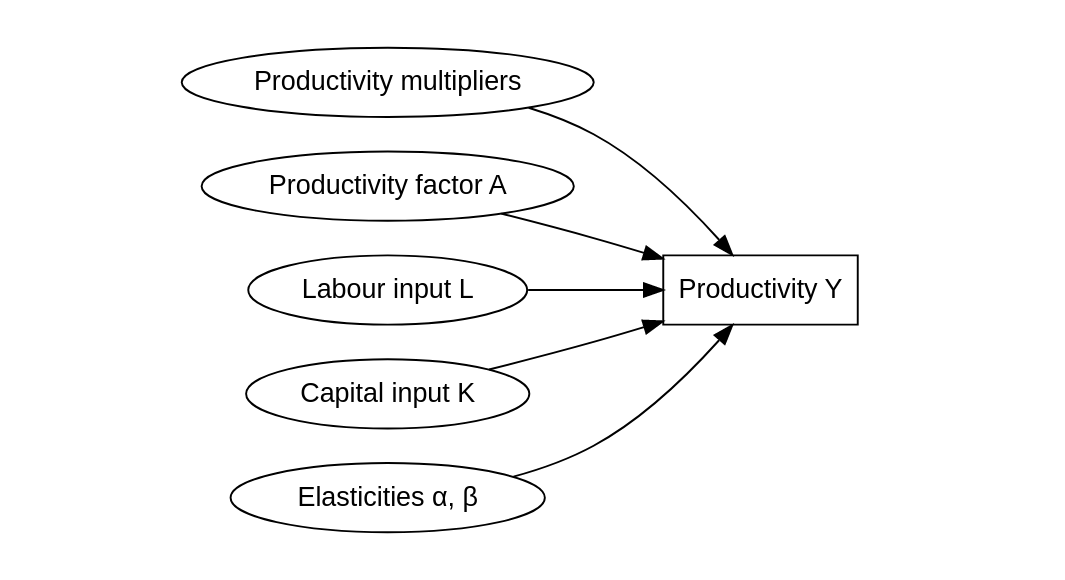
\includegraphics{Model-docs_files/figure-latex/unnamed-chunk-5-1.png}

\hypertarget{data-sources-3}{%
\section{Data sources}\label{data-sources-3}}

Data are available at \url{https://github.com/pelagikat/Local-SDGs-systems-model}

Data was obtained from Australian Bureau of Statistics
\href{https://www.abs.gov.au/statistics/economy/business-indicators/counts-australian-businesses-including-entries-and-exits/latest-release}{Counts of Australian Businesses}
and \href{https://www.abs.gov.au/websitedbs/censushome.nsf/home/tablebuilder}{Census Table Builder}

For purposes of modelling, when data refers to bin sizes (e.g., income ranges), the median value is used to represent the whole bin (e.g., for an income range of \$0 - \$50,000, the value of \$25,000 is used for all members of that data bin).

\begin{center}\rule{0.5\linewidth}{0.5pt}\end{center}

\hypertarget{equations-3}{%
\section{\texorpdfstring{\emph{Equations}}{Equations}}\label{equations-3}}

\hypertarget{agriculture-productivity-multiplier}{%
\subsection{agriculture productivity multiplier}\label{agriculture-productivity-multiplier}}

Type: Auxiliary\\
Formula: regenerative agriculture multiplier * net climate change impact on economy\\
Units: Dmnl\\
Assumptions:

\hypertarget{average-jobs-per-business-agriculture}{%
\subsection{``average jobs per business (agriculture)''}\label{average-jobs-per-business-agriculture}}

Type: Constant\\
Formula: 1.45\\
Units: jobs/structure/Year\\
Assumptions: Data from ABS (see data in Github)

\hypertarget{average-jobs-per-business-other}{%
\subsection{``average jobs per business (other)''}\label{average-jobs-per-business-other}}

Type: Constant\\
Formula: 3.66\\
Units: job/structure/Year\\
Assumptions: Data from ABS (see data in Github)

\hypertarget{average-jobs-per-business-tourism}{%
\subsection{``average jobs per business (tourism)''}\label{average-jobs-per-business-tourism}}

Type: Constant\\
Formula: 3.71\\
Units: job/structure/Year\\
Assumptions: Data from ABS (see data in Github)

\hypertarget{business-income-distribution-agriculture}{%
\subsection{``business income distribution (agriculture)''}\label{business-income-distribution-agriculture}}

Type: Constant\\
Formula: 0-\$50k = 0.3\\
\$50k-\$100k = 0.1\\
\$100k-\$200k = 0.1\\
\$200k-\$500k = 0.3\\
\$500k-\$2m = 0.1\\
\$2m-\$5m = 0\\
Units: structure*Year/dollars\\
Assumptions: This variable is split (subscripted) across 6 income cohorts. See data in Github.

\hypertarget{business-income-distribution-other}{%
\subsection{``business income distribution (other)}\label{business-income-distribution-other}}

Type: Constant\\
Formula: 0-\$50k = 0.4\\
\$50k-\$100k = 0.2\\
\$100k-\$200k = 0.2\\
\$200k-\$500k = 0.2\\
\$500k-\$2m = 0.1\\
\$2m-\$5m = 0\\
Units: structure*Year/dollars\\
Assumptions: This variable is split (subscripted) across 6 income cohorts. See data in Github.

\hypertarget{business-income-distribution-tourism}{%
\subsection{``business income distribution (tourism)}\label{business-income-distribution-tourism}}

Type: Constant\\
Formula: 0-\$50k = 0.1\\
\$50k-\$100k = 0.1\\
\$100k-\$200k = 0.1\\
\$200k-\$500k = 0.3\\
\$500k-\$2m = 0.3\\
\$2m-\$5m = 0.1\\
Units: structure*Year/dollars\\
Assumptions: This variable is split (subscripted) across 6 income cohorts. See data in Github.

\hypertarget{capital-input-ag}{%
\subsection{capital input ag}\label{capital-input-ag}}

Type: Constant\\
Formula: 2767.84\\
Units: dollars/Year\\
Assumptions: This value was calibrated against data. See data in Github.

\hypertarget{capital-input-other}{%
\subsection{capital input other}\label{capital-input-other}}

Type: Constant\\
Formula: 138131\\
Units: dollars/Year\\
Assumptions: This value was calibrated against data. See data in Github.

\hypertarget{capital-input-tourism}{%
\subsection{capital input tourism}\label{capital-input-tourism}}

Type: Constant\\
Formula: 928124\\
Units: dollars/Year\\
Assumptions: This value was calibrated against data. See data in Github.

\hypertarget{effect-of-internet-on-other-sector-business}{%
\subsection{effect of internet on other sector business}\label{effect-of-internet-on-other-sector-business}}

Type: Auxiliary\\
Formula: internet service performance / (maximum speed per connection / Fixed Wireless Towers)\\
Units: Dmnl\\
Assumptions: That poor internet performance has a negative impact on other sector businesses (which are principally home-based businesses in professional industries)

\hypertarget{effect-of-non-local-school-parents-participating-in-forrests-economy}{%
\subsection{effect of non-local school parents participating in Forrest's economy}\label{effect-of-non-local-school-parents-participating-in-forrests-economy}}

Type: Auxiliary\\
Formula: ((district kids' parents cohort / ``15-64'' ) + 1 ) * ``non-local retail demand''\\
Units: Dmnl\\
Assumptions: A multiplier which quantifies the additional traffic in Forrest as a result of transporting children to school and the effect it may have on e.g., retail business.

\hypertarget{elasticity-q1-ag}{%
\subsection{elasticity q1 ag}\label{elasticity-q1-ag}}

Type: Constant\\
Formula: 0.45\\
Units: Dmnl\\
Assumptions: calibrated against data. See data in Github.

\hypertarget{elasticity-q1-other}{%
\subsection{elasticity q1 other}\label{elasticity-q1-other}}

Type: Constant\\
Formula: 0.2\\
Units: Dmnl\\
Assumptions: calibrated against data. See data in Github.

\hypertarget{elasticity-q1-tourism}{%
\subsection{elasticity q1 tourism}\label{elasticity-q1-tourism}}

Type: Constant\\
Formula: 0.26\\
Units: Dmnl\\
Assumptions: calibrated against data. See data in Github.

\hypertarget{elasticity-q2-ag}{%
\subsection{elasticity q2 ag}\label{elasticity-q2-ag}}

Type: Constant\\
Formula: 0.01\\
Units: Dmnl\\
Assumptions: calibrated against data. See data in Github.

\hypertarget{elasticity-q2-other}{%
\subsection{elasticity q2 other}\label{elasticity-q2-other}}

Type: Constant\\
Formula: 0.74\\
Units: Dmnl\\
Assumptions: calibrated against data. See data in Github.

\hypertarget{elasticity-q2-tourism}{%
\subsection{elasticity q2 tourism}\label{elasticity-q2-tourism}}

Type: Constant\\
Formula: 0.73\\
Units: Dmnl\\
Assumptions: calibrated against data. See data in Github.

\hypertarget{fraction-of-land-under-regenerative-agriculture}{%
\subsection{fraction of land under regenerative agriculture}\label{fraction-of-land-under-regenerative-agriculture}}

Type: Constant\\
Formula: 0.05\\
Units: fraction\\
Assumptions: Actual value unknown; can be a scenario variable

\hypertarget{fraction-of-residents-in-paid-work}{%
\subsection{fraction of residents in paid work}\label{fraction-of-residents-in-paid-work}}

Type: Constant\\
Formula: Male = 0.344\\
Female = 0.424\\
Units: fraction\\
Assumptions: Data from ABS, this variable is disaggregated by gender. ABS only collects data on male/female gender so is not truly representative of gender. See data in Github.

\hypertarget{fraction-of-residents-not-in-paid-work}{%
\subsection{fraction of residents not in paid work}\label{fraction-of-residents-not-in-paid-work}}

Type: Constant\\
Formula: Male = 0.072\\
Female = 0.08\\
Units: fraction\\
Assumptions: Data from ABS, this variable is disaggregated by gender. ABS only collects data on male/female gender so is not truly representative of gender. See data in Github.

\hypertarget{fraction-of-unemployed-residents}{%
\subsection{fraction of unemployed residents}\label{fraction-of-unemployed-residents}}

Type: Constant\\
Formula: Male = 0.024\\
Female = 0.056\\
Units: fraction\\
Assumptions: Data from ABS, this variable is disaggregated by gender. ABS only collects data on male/female gender so is not truly representative of gender. See data in Github.

\hypertarget{init-ag-productivity}{%
\subsection{INIT ag productivity}\label{init-ag-productivity}}

Type: Constant\\
Formula: 1.875e+06\\
Units: dollars/Year\\
Assumptions: Data from ABS, see data in Github

\hypertarget{init-other-productivity}{%
\subsection{INIT other productivity}\label{init-other-productivity}}

Type: Constant\\
Formula: 1.175e+06\\
Units: dollars/Year\\
Assumptions: Data from ABS, see data in Github

\hypertarget{init-tourism-productivity}{%
\subsection{INIT tourism productivity}\label{init-tourism-productivity}}

Type: Constant\\
Formula: 25000\\
Units: dollars/Year\\
Assumptions: Data from ABS, see data in Github

\hypertarget{job-vacancies-agriculture-filled-externally}{%
\subsection{``job vacancies (agriculture) filled externally''}\label{job-vacancies-agriculture-filled-externally}}

Type: Auxiliary\\
Formula: IF THEN ELSE(``labour demand (agriculture)'' \textgreater{} labour input ag, ``labour demand (agriculture)'' - labour input ag, 0)\\
Units: job/Year\\
Assumptions: This variable represents the number of jobs within Forrest that require non-local employees

\hypertarget{job-vacancies-other-filled-externally}{%
\subsection{``job vacancies (other) filled externally''}\label{job-vacancies-other-filled-externally}}

Type: Auxiliary\\
Formula: IF THEN ELSE(``labour demand (other)'' \textgreater{} labour input other, ``labour demand (other)'' - labour input other, 0)\\
Units: job/Year\\
Assumptions: This variable represents the number of jobs within Forrest that require non-local employees

\hypertarget{job-vacancies-tourism-filled-externally}{%
\subsection{``job vacancies (tourism) filled externally''}\label{job-vacancies-tourism-filled-externally}}

Type: Auxiliary\\
Formula: IF THEN ELSE(``labour demand (tourism)'' \textgreater{} labour input tourism, ``labour demand (tourism)'' - labour input tourism, 0)\\
Units: job/Year\\
Assumptions: This variable represents the number of jobs within Forrest that require non-local employees

\hypertarget{labour-demand-agriculture}{%
\subsection{``labour demand (agriculture)''}\label{labour-demand-agriculture}}

Type: Auxiliary\\
Formula: ``number of businesses (agriculture)'' * ``average jobs per business (agriculture)''\\
Units: job/Year\\
Assumptions:

\hypertarget{labour-demand-other}{%
\subsection{``labour demand (other)''}\label{labour-demand-other}}

Type: Auxiliary\\
Formula: ``average jobs per business (other)''*``number of businesses (other)''\\
Units: job/Year\\
Assumptions:

\hypertarget{labour-demand-tourism}{%
\subsection{``labour demand (tourism)''}\label{labour-demand-tourism}}

Type: Auxiliary\\
Formula: ``number of businesses (tourism)'' * ``average jobs per business (tourism)''\\
Units: job/Year\\
Assumptions:

\hypertarget{labour-force}{%
\subsection{labour force}\label{labour-force}}

Type: Auxiliary\\
Formula: Male = residents in paid work{[}Male{]} + unemployed residents{[}Male{]}\\
Female = residents in paid work{[}Female{]} + unemployed residents{[}Female{]}\\
Units: people\\
Assumptions: This variable is disaggregated by gender. ABS only collects data on male/female gender so is not truly representative of gender.

\hypertarget{labour-input-ag}{%
\subsection{labour input ag}\label{labour-input-ag}}

Type: Auxiliary\\
Formula: sum(labour force {[}Gender!{]}) * ``reference jobs fraction (agriculture)''\\
Units: job/Year\\
Assumption: This variable re-aggregates the gender disaggregated variables

\hypertarget{labour-input-other}{%
\subsection{labour input other}\label{labour-input-other}}

Type: Auxiliary\\
Formula: sum(labour force {[}Gender!{]}) * ``reference jobs fraction (other)''\\
Units: job/Year\\
Assumption: This variable re-aggregates the gender disaggregated variables

\hypertarget{labour-input-tourism}{%
\subsection{labour input tourism}\label{labour-input-tourism}}

Type: Auxiliary\\
Formula: sum(labour force {[}Gender!{]}) * ``reference jobs fraction (tourism)''\\
Units: job/Year\\
Assumption: This variable re-aggregates the gender disaggregated variables

\hypertarget{non-local-retail-demand}{%
\subsection{``non-local retail demand''}\label{non-local-retail-demand}}

Type: Constant\\
Formula: 1.2\\
Units: Dmnl\\
Assumptions: Actual value unknown; can be a scenario variable

\hypertarget{number-of-businesses-agriculture}{%
\subsection{``number of businesses (agriculture)''}\label{number-of-businesses-agriculture}}

Type: Auxiliary\\
Formula: INTEGER( sum (``number of businesses in income bracket (agriculture)''{[}Business Income!{]}))\\
Units: structure\\
Assumptions: this variable sums the agriculture businesses in all income brackets to arrive at an integer value

\hypertarget{number-of-businesses-other}{%
\subsection{``number of businesses (other)''}\label{number-of-businesses-other}}

Type: Auxiliary\\
Formula: INTEGER( sum (``number of businesses in income bracket (other)''{[}Business Income!{]}))\\
Units: structure\\
Assumptions: this variable sums the other businesses in all income brackets to arrive at an integer value

\hypertarget{number-of-businesses-tourism}{%
\subsection{``number of businesses (tourism)''}\label{number-of-businesses-tourism}}

Type: Auxiliary\\
Formula: INTEGER( sum (``number of businesses in income bracket (tourism)''{[}Business Income!{]}))\\
Units: structure
Assumptions: this variable sums the tourism businesses in all income brackets to arrive at an integer value

\hypertarget{number-of-businesses-in-income-bracket-agriculture}{%
\subsection{``number of businesses in income bracket (agriculture)''}\label{number-of-businesses-in-income-bracket-agriculture}}

Type: Auxiliary\\
Formula: 0-\$50k = (``business income distribution (agriculture)''{[}``0-\$50k''{]} * Total Agricultural Productivity) / 25000\\
\$50k-\$100k = (``business income distribution (agriculture)''{[}``\$50k-\$100k''{]} * Total Agricultural Productivity) / 75000\\
\$100k-\$200k = (``business income distribution (agriculture)''{[}``\$100k-\$200k''{]} * Total Agricultural Productivity) / 150000\\
\$200k-\$500k = (``business income distribution (agriculture)''{[}``\$200k-\$500k''{]} * Total Agricultural Productivity) / 350000\\
\$500k-\$2m = (``business income distribution (agriculture)''{[}``\$500k-\$2m''{]} * Total Agricultural Productivity) / 1.25e+06\\
\$2m-\$5m = (``business income distribution (agriculture)''{[}``\$2m-\$5m''{]} * Total Agricultural Productivity) / 3.5e+06\\
Units: structure\\
Assumptions: This variable is split (subscripted) across 6 income cohorts. Median values used for each for income bracket divisor.

\hypertarget{number-of-businesses-in-income-bracket-other}{%
\subsection{``number of businesses in income bracket (other)''}\label{number-of-businesses-in-income-bracket-other}}

Type: Auxiliary\\
Formula: 0-\$50k = (``business income distribution (other)''{[}``0-\$50k''{]} * Total Agricultural Productivity) / 25000\\
\$50k-\$100k = (``business income distribution (other)''{[}``\$50k-\$100k''{]} * Total Agricultural Productivity) / 75000\\
\$100k-\$200k = (``business income distribution (other)''{[}``\$100k-\$200k''{]} * Total Agricultural Productivity) / 150000\\
\$200k-\$500k = (``business income distribution (other)''{[}``\$200k-\$500k''{]} * Total Agricultural Productivity) / 350000\\
\$500k-\$2m = (``business income distribution (other)''{[}``\$500k-\$2m''{]} * Total Agricultural Productivity) / 1.25e+06\\
\$2m-\$5m = (``business income distribution (other)''{[}``\$2m-\$5m''{]} * Total Agricultural Productivity) / 3.5e+06\\
Units: structure\\
Assumptions: This variable is split (subscripted) across 6 income cohorts. Median values used for each for income bracket divisor.

\hypertarget{number-of-businesses-in-income-bracket-tourism}{%
\subsection{``number of businesses in income bracket (tourism)''}\label{number-of-businesses-in-income-bracket-tourism}}

Type: Auxiliary\\
Formula: 0-\$50k = (``business income distribution (tourism)''{[}``0-\$50k''{]} * Total Agricultural Productivity) / 25000\\
\$50k-\$100k = (``business income distribution (tourism)''{[}``\$50k-\$100k''{]} * Total Agricultural Productivity) / 75000\\
\$100k-\$200k = (``business income distribution (tourism)''{[}``\$100k-\$200k''{]} * Total Agricultural Productivity) / 150000\\
\$200k-\$500k = (``business income distribution (tourism)''{[}``\$200k-\$500k''{]} * Total Agricultural Productivity) / 350000\\
\$500k-\$2m = (``business income distribution (tourism)''{[}``\$500k-\$2m''{]} * Total Agricultural Productivity) / 1.25e+06\\
\$2m-\$5m = (``business income distribution (tourism)''{[}``\$2m-\$5m''{]} * Total Agricultural Productivity) / 3.5e+06\\
Units: structure\\
Assumptions: This variable is split (subscripted) across 6 income cohorts. Median values used for each for income bracket divisor.

\hypertarget{other-productivity-multiplier}{%
\subsection{other productivity multiplier}\label{other-productivity-multiplier}}

Type: Auxiliary\\
Formula: effect of internet on other sector business * ``effect of non-local school parents participating in Forrest's economy''\\
Units: Dmnl\\
Assumptions:

\hypertarget{productivity-factor-ag}{%
\subsection{productivity factor ag}\label{productivity-factor-ag}}

Type: Constant\\
Formula: 145.7\\
Units: 1/job\\
Assumptions: calibrated against data. See data in Github.

\hypertarget{productivity-factor-other}{%
\subsection{productivity factor other}\label{productivity-factor-other}}

Type: Constant\\
Formula: 700\\
Units: 1/job\\
Assumptions: calibrated against data. See data in Github.

\hypertarget{productivity-factor-tourism}{%
\subsection{productivity factor tourism}\label{productivity-factor-tourism}}

Type: Constant\\
Formula: 421.7\\
Units: 1/job\\
Assumptions: calibrated against data. See data in Github.

\hypertarget{profitability-increase-from-regenerative-agriculture}{%
\subsection{profitability increase from regenerative agriculture}\label{profitability-increase-from-regenerative-agriculture}}

Type: Auxiliary\\
Formula: RA coefficient*Time +RA intercept\\
Units: Dmnl\\
Assumptions: Linear model from NSW data - \citet{ogilvy_graziers_2018}

\hypertarget{ra-coefficient}{%
\subsection{RA coefficient}\label{ra-coefficient}}

Type: Constant\\
Formula: -0.034\\
Units: Dmnl\\
Assumptions: Calculated from data. See Github for data and derivation of linear model.

\hypertarget{ra-intercept}{%
\subsection{RA intercept}\label{ra-intercept}}

Type: Constant\\
Formula: 69.8\\
Units: Dmnl\\
Assumptions: Calculated from data. See Github for data and derivation of linear model.

\hypertarget{rate-of-productivity-change-ag}{%
\subsection{Rate of productivity change ag}\label{rate-of-productivity-change-ag}}

Type: Auxiliary\\
Formula: agriculture productivity multiplier * productivity factor ag * (capital input ag \^{} elasticity q1 ag) * (labour input ag \^{} elasticity q2 ag)\\
Units: dollars/(Year*Year)\\
Assumptions: the Cobb-Douglas production function

\hypertarget{rate-of-productivity-change-other}{%
\subsection{Rate of productivity change other}\label{rate-of-productivity-change-other}}

Type: Auxiliary\\
Formula: other productivity multiplier * productivity factor other * ( capital input other \^{} elasticity q1 other) * (labour input other \^{} elasticity q2 other)\\
Units: dollars/(Year*Year)\\
Assumptions: the Cobb-Douglas production function

\hypertarget{rate-of-productivity-change-tourism}{%
\subsection{Rate of productivity change tourism}\label{rate-of-productivity-change-tourism}}

Type: Auxiliary\\
Formula: tourism productivity multiplier * productivity factor tourism * (capital input tourism \^{} elasticity q1 tourism) * (labour input tourism \^{} elasticity q2 tourism)\\
Units: dollars/(Year*Year)\\
Assumptions: the Cobb-Douglas production function

\hypertarget{reference-jobs-fraction-agriculture}{%
\subsection{``reference jobs fraction (agriculture)''}\label{reference-jobs-fraction-agriculture}}

Type: Constant\\
Formula: 0.18\\
Units: job/people/Year\\
Assumptions: calibrated against data. See data in Github.

\hypertarget{reference-jobs-fraction-other}{%
\subsection{``reference jobs fraction (other)''}\label{reference-jobs-fraction-other}}

Type: Constant\\
Formula: 0.22\\
Units: job/people/Year\\
Assumptions: calibrated against data. See data in Github.

\hypertarget{reference-jobs-fraction-tourism}{%
\subsection{``reference jobs fraction (tourism)''}\label{reference-jobs-fraction-tourism}}

Type: Constant\\
Formula: 0.279638\\
Units: job/people/Year\\
Assumptions: calibrated against data. See data in Github.

\hypertarget{regenerative-agriculture-multiplier}{%
\subsection{regenerative agriculture multiplier}\label{regenerative-agriculture-multiplier}}

Type: Auxiliary\\
Formula: 1 + (fraction of land under regenerative agriculture * profitability increase from regenerative agriculture)\\
Units: Dmnl\\
Assumptions: calibrated against data. See data in Github.

\hypertarget{residents-in-paid-work}{%
\subsection{residents in paid work}\label{residents-in-paid-work}}

Type: Auxiliary\\
Formula: Male = fraction of residents in paid work{[}Male{]} * ``working-age population''\\
Female = fraction of residents in paid work{[}Female{]} * ``working-age population''\\
Units: people
Assumptions: Data from ABS, disaggregated by gender (only two categories), ``Employed, worked x-time'' categories. See data in Github.

\hypertarget{residents-not-in-paid-work}{%
\subsection{residents not in paid work}\label{residents-not-in-paid-work}}

Type: Auxiliary\\
Formula: Male = fraction of residents not in paid work{[}Male{]} * ``working-age population''\\
Female = fraction of residents not in paid work{[}Female{]} * ``working-age population''\\
Units: people
Assumptions: Data from ABS, disaggregated by gender (only two categories), ABS ``Away From Work'' category. See data in Github.

\hypertarget{total-agricultural-productivity}{%
\subsection{Total Agricultural Productivity}\label{total-agricultural-productivity}}

Type: Stock\\
Formula: INTEG ( Rate of productivity change ag), INITIAL = INIT ag productivity\\
Units: dollars/Year\\
Assumptions:

\hypertarget{total-other-productivity}{%
\subsection{Total Other Productivity}\label{total-other-productivity}}

Type: Stock\\
Formula: INTEG ( Rate of productivity change other), INITIAL = INIT other productivity\\
Units: dollars/Year\\
Assumptions:

\hypertarget{total-productivity}{%
\subsection{total productivity}\label{total-productivity}}

Type: Auxiliary\\
Formula: Total Agricultural Productivity + Total Other Productivity + Total Tourism Productivity\\
Units: dollar/Year\\
Assumptions: Sum of all total productivity stocks

\hypertarget{total-tourism-productivity}{%
\subsection{Total Tourism Productivity}\label{total-tourism-productivity}}

Type: Stock\\
Formula: INTEG (Rate of productivity change tourism), INITAL = INIT tourism productivity)\\
Units: dollars/Year\\
Assumptions:

\hypertarget{tourism-productivity-multiplier}{%
\subsection{tourism productivity multiplier}\label{tourism-productivity-multiplier}}

Type: Auxiliary\\
Formula: Number Of Tourists / normal tourist numbers\\
Units: Dmnl\\
Assumptions:

\hypertarget{unemployed-residents}{%
\subsection{unemployed residents}\label{unemployed-residents}}

Type: Auxiliary\\
Formula: Male = fraction of unemployed residents{[}Male{]} * ``working-age population''\\
Female = fraction of unemployed residents{[}Female{]} * ``working-age population''\\
Units: people\\
Assumptions: Data from ABS, disaggregated by gender (only two categories), looking for x-time work'' categories. See data in Github.

\hypertarget{unemployment-agriculture}{%
\subsection{``unemployment (agriculture)''}\label{unemployment-agriculture}}

Type: Auxiliary\\
Formula: IF THEN ELSE(``labour demand (agriculture)'' \textless{} labour input ag, labour input ag - ``labour demand (agriculture)'', 0)\\
Units: job/Year\\
Assumptions:

\hypertarget{unemployment-other}{%
\subsection{``unemployment (other)''}\label{unemployment-other}}

Type: Auxiliary\\
Formula: IF THEN ELSE(``labour demand (other)'' \textless{} labour input other, labour input other - ``labour demand (other)'', 0)\\
Units: job/Year\\
Assumptions:

\hypertarget{unemployment-tourism}{%
\subsection{``unemployment (tourism)''}\label{unemployment-tourism}}

Type: Auxiliary\\
Formula: IF THEN ELSE(``labour demand (tourism)'' \textless{} labour input tourism, labour input tourism - ``labour demand (tourism)'', 0)\\
Units: job/Year\\
Assumptions

\hypertarget{working-age-population}{%
\subsection{``working-age population''}\label{working-age-population}}

Type: Auxiliary\\
Formula: ``15-64''\\
Units: people\\
Assumptions: this is a renaming of the ``15-64'' age cohort to make clear it is explicitly the population of Forrest who are of working age.

\hypertarget{tourism-component}{%
\chapter{Tourism component}\label{tourism-component}}

\hypertarget{problem-definition-4}{%
\section{\texorpdfstring{\emph{Problem definition}}{Problem definition}}\label{problem-definition-4}}

\begin{enumerate}
\def\labelenumi{\arabic{enumi}.}
\tightlist
\item
  Forrest's major tourism drawcards are its beautiful natural environment and the Mountain Bike Trails. It follows that these are also its vulnerabilities.
\end{enumerate}

\emph{Dynamic hypothesis:}
Tourist numbers are affected by the incidence of bushfire either locally or elsewhere in Victoria, by flooding, and by the quality of local infrastructure (including the MTB trails and wastewater).

\begin{enumerate}
\def\labelenumi{\arabic{enumi}.}
\setcounter{enumi}{1}
\tightlist
\item
  Because tourism accommodation is primarily sourced from residential housing stock, neither residential housing nor dedicated tourism accommodation is able to be built because of the wastewater problem.
\end{enumerate}

\emph{Dynamic hypothesis:}
The current state of wastewater in Forrest impacts the development of housing and tourism accommodation, thus impacting growth in tourist numbers.

\begin{enumerate}
\def\labelenumi{\arabic{enumi}.}
\setcounter{enumi}{2}
\tightlist
\item
  Forrest is virtually inaccessible unless you have a car, thus is excluded from tourists who do not drive.
\end{enumerate}

\emph{Dynamic hypothesis:}
The frequency of bus services in Forrest is inadequate for residents, let alone to support tourist movement. An increase in bus frequency would enable growth in tourist numbers.

\hypertarget{system-conceptualisation-2}{%
\section{\texorpdfstring{\emph{System conceptualisation}}{System conceptualisation}}\label{system-conceptualisation-2}}

Tourism already exists as part of the Economy component, so here we are not modelling the finances of tourism, but instead we want to explore what effect external factors may have on tourist numbers.

\hypertarget{conceptual-model-4}{%
\subsection{Conceptual model}\label{conceptual-model-4}}

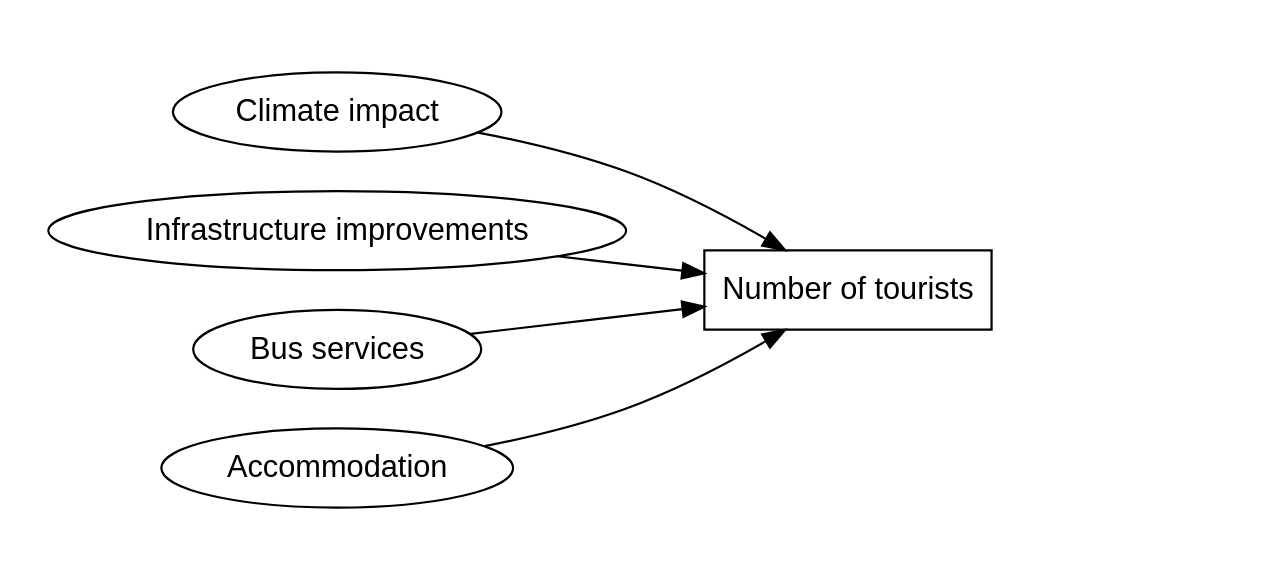
\includegraphics{Model-docs_files/figure-latex/unnamed-chunk-6-1.png}

\hypertarget{model-formulation-2}{%
\section{\texorpdfstring{\emph{Model formulation}}{Model formulation}}\label{model-formulation-2}}

Here our stock variable is the Number of Tourists, with a flow of Rate of tourist increase. Affecting that flow rate are climate disasters, tourism accommodation, infrastructure improvement, and bus frequency.

\begin{center}\rule{0.5\linewidth}{0.5pt}\end{center}

\hypertarget{equations-4}{%
\section{\texorpdfstring{\emph{Equations}}{Equations}}\label{equations-4}}

\hypertarget{effect-of-future-improvements-to-infrastructure}{%
\subsection{effect of future improvements to infrastructure}\label{effect-of-future-improvements-to-infrastructure}}

Type: Constant\\
Formula: 1\\
Units: Dmnl\\
Assumptions: Scenario variable to model unknown changes

\hypertarget{effect-of-mtb-trails-improvements}{%
\subsection{effect of MTB Trails improvements}\label{effect-of-mtb-trails-improvements}}

Type: Auxiliary\\
Formula: IF THEN ELSE(MTB trails improvements availability \textgreater{} 0, 1.5, 1)\\
Units: Dmnl\\
Assumptions: Cost benefit analysis of mountain bike trail improvements: increase of 25,000 cycling tourists per annum from 24,000 (doubling). Assume that only half of these stay in Forrest.

\hypertarget{effect-of-wastewater}{%
\subsection{effect of wastewater}\label{effect-of-wastewater}}

Type: Auxiliary\\
Formula: IF THEN ELSE(Wastewater availability \textgreater{} 0, 2, 1)\\
Units: Dmnl\\
Assumptions: Assume a doubling of tourists from improved wastewater infrastructure

\hypertarget{impact-of-bus-frequency-on-tourist-numbers}{%
\subsection{impact of bus frequency on tourist numbers}\label{impact-of-bus-frequency-on-tourist-numbers}}

Type: Auxiliary\\
Formula: IF THEN ELSE(tourist bus frequency \textgreater{} 1 :AND: Time \textgreater{} 2006, ( 1 + ((tourist bus frequency * tourist bus capacity) / Number Of Tourists)) , 1)\\
Units: Dmnl\\
Assumptions: modelling for tourist buses that do not currently exist.

\hypertarget{impact-of-climate-on-tourism}{%
\subsection{impact of climate on tourism}\label{impact-of-climate-on-tourism}}

Type: Auxiliary\\
Formula: 1- (( 1 - bushfire risk fraction) + probability of catastrophic bushfire elsewhere in Victoria - annual probability of flood)\\
Units: Dmnl\\
Assumptions: local bushfire risk and flooding is a negative impact, bushfire elsewhere is a positive impact

\hypertarget{impact-of-tourism-infrastructure-improvements-on-tourist-numbers}{%
\subsection{impact of tourism infrastructure improvements on tourist numbers}\label{impact-of-tourism-infrastructure-improvements-on-tourist-numbers}}

Type: Auxiliary\\
Formula: effect of MTB Trails improvements * effect of wastewater * effect of future improvements to infrastructure\\
Units: Dmnl\\
Assumptions: that infrastructure improvements will each have an independent effect on tourist numbers

\hypertarget{initial-tourist-increase}{%
\subsection{initial tourist increase}\label{initial-tourist-increase}}

Type: Auxiliary\\
Formula: RAMP(100, 2000, 2006 )\\
Units: people/Year\\
Assumptions: tourism did not commence in Forrest in earnest until 2006, so this is a value to show a small increase in tourist numbers over the period 2000 - 2006.

\hypertarget{normal-tourist-numbers}{%
\subsection{normal tourist numbers}\label{normal-tourist-numbers}}

Type: Constant\\
Formula: 3432\\
Units: people/Year\\
Assuming 33 houses in Forrest used for tourism (2006 census unoccupied dwellings), at an average of 3 night stays, this means Forrest's houses can support a max of 6000 tourists per year. Make an assumption that houses will only be occupied on weekends (for ``normal'' numbers), multiplied by two for two-people-per-house stays: 33 * 52 * 2 approx = 3232 people per year

\hypertarget{number-of-tourists}{%
\subsection{Number Of Tourists}\label{number-of-tourists}}

Type: Stock\\
Formula: INTEG (Rate of tourist increase), INITIAL = 0)\\
Units: people/Year\\
Assumptions:

\hypertarget{probability-of-catastrophic-bushfire-elsewhere-in-victoria}{%
\subsection{probability of catastrophic bushfire elsewhere in Victoria}\label{probability-of-catastrophic-bushfire-elsewhere-in-victoria}}

Type: Constant\\
Formula: 0.1\\
Units: Dmnl\\
Assumptions: Assume 1 catastrophic bushfire every ten years elsewhere in Victoria (prior data: 1983, 1998, 2009, 2020)

\hypertarget{rate-of-tourist-increase}{%
\subsection{Rate of tourist increase}\label{rate-of-tourist-increase}}

Type: Auxiliary\\
Formula: IF THEN ELSE ( Time \textgreater{} 2006 :AND: tourist house discrepancy \textgreater{} 0, tourist house discrepancy * average size of household * tourist numbers multiplier, initial tourist increase )\\
Units: people/Year\\
Assumptions: An if-then-else formula to represent the pre- and post-2006 states of tourism in Forrest

\hypertarget{tourist-bus-capacity}{%
\subsection{tourist bus capacity}\label{tourist-bus-capacity}}

Type: Constant\\
Formula: 25\\
Units: people/bus\\
Assumptions: Assume same size bus as public transport

\hypertarget{tourist-bus-frequency}{%
\subsection{tourist bus frequency}\label{tourist-bus-frequency}}

Type: Constant\\
Formula: 0\\
Units: bus/Year\\
Assumptions: Currently no buses run; this can be a scenario variable

\hypertarget{tourist-house-discrepancy}{%
\subsection{tourist house discrepancy}\label{tourist-house-discrepancy}}

Type: Auxiliary\\
Formula: (Tourism Housing * number of times each tourist house occupied per year - (Number Of Tourists / average size of household ))\\
Units: structure/Year\\
Assumptions: a supply vs demand variable

\hypertarget{tourist-numbers-multiplier}{%
\subsection{tourist numbers multiplier}\label{tourist-numbers-multiplier}}

Type: Auxiliary\\
Formula: SMOOTH3 ( impact of tourism infrastructure improvements on tourist numbers * impact of climate on tourism * impact of bus frequency on tourist numbers , 10 )\\
Units: Dmnl\\
Assumptions: A smoothing function to show a gradual impact change over time from various impact inputs

\hypertarget{biodiversity-component}{%
\chapter{Biodiversity component}\label{biodiversity-component}}

\hypertarget{problem-definition-5}{%
\section{\texorpdfstring{\emph{Problem definition}}{Problem definition}}\label{problem-definition-5}}

Forrest is located in a biodiversity hotspot, and the Great Otway National Park provides protection for some of that biodiversity. The local residents are proud of their pristine surroundings and dedicated to ensuring they remain so. Climate change and potential bushfire impact are both threats to the local environment, as well as any land use change which reduces the amount of bushland. Fertiliser runoff from agriculture is also a potential danger.

\emph{Dynamic hypothesis:}
Climate change and land use change are the fundamental drivers for biodiversity risk. They both increases bushfire risk and land use change reduces habitat. Indigenous cultural burning may be a way to mitigate biodiversity loss (by healing Country) but has a significant lead-in/preparation time.

\hypertarget{system-conceptualisation-and-model-formulation-1}{%
\section{\texorpdfstring{\emph{System conceptualisation and model formulation}}{System conceptualisation and model formulation}}\label{system-conceptualisation-and-model-formulation-1}}

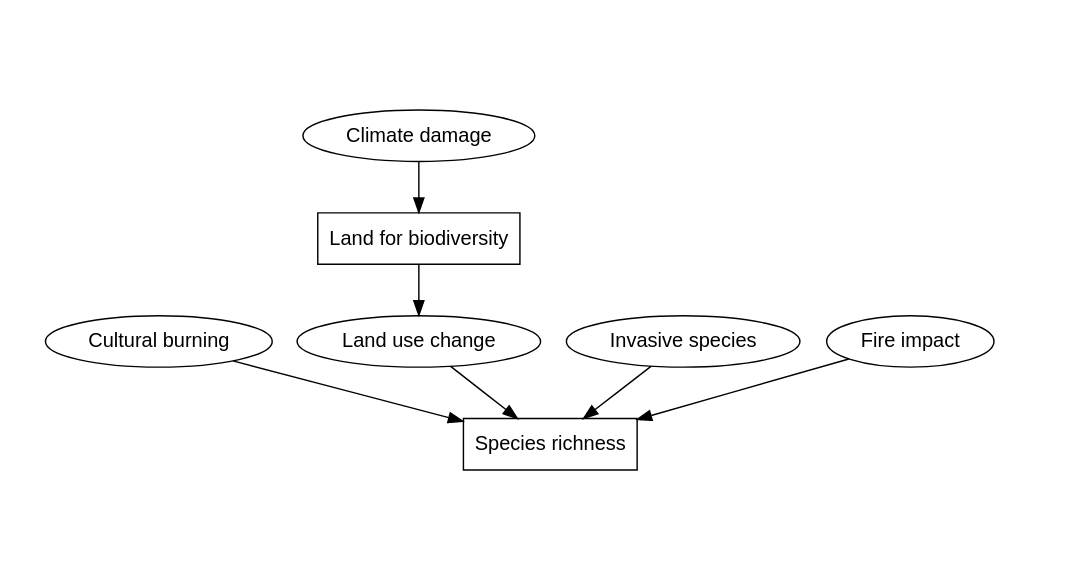
\includegraphics{Model-docs_files/figure-latex/unnamed-chunk-7-1.png}

Species richness is the critical variable in the biodiversity component. Species richness can be affected by cultural burning, land use change, invasive species and climate change. Land use change is modelled using a species area curve,
\[
S = cA^z 
\]

where Z = 0.86 (derived from data), A = land area, c = constant, and S = number of species.

Land use for biodiversity purposes is modelled as a stock and flow structure to accurately represent the impact of climate damage on land area for biodiversity. We assume that agricultural land does not support biodiversity for simplicity.

\hypertarget{data-sources-4}{%
\section{Data sources}\label{data-sources-4}}

Data are available at \url{https://github.com/pelagikat/Local-SDGs-systems-model}

These data represent only those species that have data on the Atlas of Living Australia and have passed a data cleaning process. It likely represents about 40-50\% of terrestrial vertebrate and vascular plant species (\citet{graham_climate_2019}). The underlying information that these data represent is climate suitability. For each species, climate variables were used to project suitability of cells across Australia for species based on current climate ranges (cells receive a value between 0-1). To create the species richness map, cells that were projected with values greater than 0.5 were classified into a binary value of 1. All species rasters were then spatially added within each taxonomic group. See \url{https://github.com/CarlaBirdy/MaxEnt-climate-models} for the code for this analysis.

Thanks to Carla Archibald for assisting with data for this model component.

\begin{center}\rule{0.5\linewidth}{0.5pt}\end{center}

\hypertarget{equations-5}{%
\section{\texorpdfstring{\emph{Equations}}{Equations}}\label{equations-5}}

\hypertarget{baseline-invasive-species-impact}{%
\subsection{baseline invasive species impact}\label{baseline-invasive-species-impact}}

Type: Auxiliary\\
Formula: INIT species richness - (0.21*INIT species richness)\\
Units: species\\
Assumptions: 21\% species richnesss decline compared to natural systems; \citet{crystal-ornelas_cumulative_2020}

\hypertarget{fire-impact-on-biodiversity}{%
\subsection{fire impact on biodiversity}\label{fire-impact-on-biodiversity}}

Type: Auxiliary\\
Formula: 1 + (1 - (1/FFDI model))\\
Units: Dmnl\\
Assumptions:

\hypertarget{impact-of-climate-damage-on-biodiversity}{%
\subsection{impact of climate damage on biodiversity}\label{impact-of-climate-damage-on-biodiversity}}

Type: Auxiliary\\
Formula: 0.00091\\
Units: Dmnl\\
Assumptions: Climate damage for Forrest area from LUTO model. Land suitable for biodiversity reduces by 10\% between 1990 and 2100, therefore annualised reduction is 9.1e-4 \%

\hypertarget{impact-of-cultural-burning-on-biodiversity}{%
\subsection{impact of cultural burning on biodiversity}\label{impact-of-cultural-burning-on-biodiversity}}

Type: Auxiliary\\
Formula: 1+Cultural Burning\\
Units: Dmnl\\
Assumptions: In personal discussions with an Australian fire researcher, they suggested that cultural burning would have a positive impact on biodiversity compared with a fire suppression regime (business as usual). Some evidence provided by \citet{bowman_human_2011}, \citet{trauernicht_local_2015}.

\hypertarget{init-species-richness}{%
\subsection{INIT species richness}\label{init-species-richness}}

Type: Constant\\
Formula: 4637\\
Units: species\\
Assumptions: Baseline 1990 data for species richness in the Colac Otway LGA area. Includes amphibians, birds, mammals, plants and reptiles. See Github for spatial data.

\hypertarget{invasive-species-impact-discrepancy}{%
\subsection{invasive species impact discrepancy}\label{invasive-species-impact-discrepancy}}

Type: Auxiliary\\
Formula: Species richness-baseline invasive species impact\\
Units: species\\
Assumptions:

\hypertarget{land-for-biodiversity-impact}{%
\subsection{Land for Biodiversity Impact}\label{land-for-biodiversity-impact}}

Type: Stock\\
Formula: INTEG( Land use change over time - Land reduction from climate damage), INITIAL = 0\\
Units: hectares\\
Assumptions:

\hypertarget{land-use-change-impact-on-biodiversity}{%
\subsection{land use change impact on biodiversity}\label{land-use-change-impact-on-biodiversity}}

Type: Auxiliary\\
Formula: (species area curve coefficient * Land for Biodiversity Impact \^{} species area curve exponent) / simulation time\\
Units: species/Year\\
Assumptions: Species area curve S = cA\^{}z , z = 0.86 (derived from data). Assume that species richness initial variable is 50\% of total c = 2 Area = 8375 S = 4637

\hypertarget{land-use-change-over-time}{%
\subsection{Land use change over time}\label{land-use-change-over-time}}

Type: Auxiliary\\
Formula: (Forest Land + Protected Land) / simulation time\\
Units: hectares/Year\\
Assumptions: Agricultural land has no biodiversity impact

\hypertarget{land-reduction-from-climate-damage}{%
\subsection{Land reduction from climate damage}\label{land-reduction-from-climate-damage}}

Type: Auxiliary\\
Formula: Land for Biodiversity Impact * impact of climate on biodiversity\\
Units: hectares/Year\\
Assumptions:

\hypertarget{species-area-curve-coefficient}{%
\subsection{species area curve coefficient}\label{species-area-curve-coefficient}}

Type: Constant\\
Formula: 2\\
Units: species/hectares\\
Assumptions: as derived in \emph{land use change impact on biodiversity}

\hypertarget{species-area-curve-exponent}{%
\subsection{species area curve exponent}\label{species-area-curve-exponent}}

Type: Constant\\
Formula: 0.86\\
Units: Dmnl\\
Assumptions: derived from data

\hypertarget{species-richness}{%
\subsection{Species richness}\label{species-richness}}

Type: Stock\\
Formula: INTEG (Species richness increase rate - Species richness decrease rate), INITIAL = INIT species richness)\\
Units: species\\
Assumptions:

\hypertarget{species-richness-decrease-rate}{%
\subsection{Species richness decrease rate}\label{species-richness-decrease-rate}}

Type: Auxiliary\\
Formula: (invasive species impact discrepancy / simulation time) * fire impact on biodiversity\\
Units: species/Year\\
Assumptions:

\hypertarget{species-richness-increase-rate}{%
\subsection{Species richness increase rate}\label{species-richness-increase-rate}}

Type: Auxiliary\\
Formula: impact of cultural burning on biodiversity * land use change impact on biodiversity\\
Units: species/Year\\
Assumptions:

\hypertarget{climate-change-component}{%
\chapter{Climate change component}\label{climate-change-component}}

\hypertarget{problem-definition-6}{%
\section{\texorpdfstring{\emph{Problem definition}}{Problem definition}}\label{problem-definition-6}}

\begin{enumerate}
\def\labelenumi{\arabic{enumi}.}
\tightlist
\item
  Human-induced climate change is a problem that will require a united, global effort to combat. However, the effects of climate change do and will continue to affect Forrest at a community level. Such affects include increasing temperatures, drying climates, increased and more serious bushfires, droughts, and more extreme weather. To remain safe and stay resilient in the face of climate change, Forrest must anticipate more frequent bushfires, flooding and drought, and develop plans for sustainable recovery.
\end{enumerate}

\emph{Dynamic hypothesis:}

Forrest is vulnerable to bushfires and drought, and the effect of climate change on biodiversity may begin to affect Forrest's eco-tourism economy. Increasing temperatures will also affect Forrest's residents, especially as the community is ageing. More frequent heatwaves will put older people, more susceptible to heat-induced illness, at risk. Forrest is occasionally subject to flooding (e.g.~the spillover of Barwon Dam in 2012), and with the increase in extreme weather events this could become more frequent.

\hypertarget{system-conceptualisation-3}{%
\section{\texorpdfstring{\emph{System conceptualisation}}{System conceptualisation}}\label{system-conceptualisation-3}}

There are four climate-related models that make up the climate change component, with a separate structure for cultural burning. These four models are for carbon dioxide, temperature, rainfall, and bushfire.

\hypertarget{model-formulation-3}{%
\section{\texorpdfstring{\emph{Model formulation}}{Model formulation}}\label{model-formulation-3}}

For each of the four climate models, we generated linear models based on past data. The rainfall model is for annual rainfall; the temperature model is for annual mean maximum temperature; the CO\textsubscript{2} model is for monthly CO\textsubscript{2} measurements; and for bushfire we modelled the annual mean Forest Fire Danger Index (\citet{matthews_comparison_2009}) for the Forrest area. The linear models were created using data from 1990-2020.

The climate damage structure was adapted from FeliX (\citet{rydzak_impact_2010}).

The cultural burning structure represents the percentage of land that is managed by cultural burning. The initial value is 0 and the model is `switched' on or off depending on scenario. The cultural burning goal is set as 100\%.

\hypertarget{data-sources-5}{%
\section{Data sources}\label{data-sources-5}}

Data and code are available at \url{https://github.com/pelagikat/Local-SDGs-systems-model}

CO\textsubscript{2} data was obtained from the \href{https://www.csiro.au/en/research/natural-environment/atmosphere/latest-greenhouse-gas-data}{Cape Grim monitoring station}

Temperature and rainfall data was obtained from the \href{http://www.bom.gov.au/climate/data/?ref=ftr}{Bureau of Meteorology}. Temperature data was from the Cape Otway weather station, and rainfall data was from the Pennyroyal weather station. These stations were selected as they were both the most complete and spatially nearest datasets available.

Forest Fire Danger Index historical data was provided from the Victorian Government Department of Land, Water and Planning ViCClim dataset. Data was extracted from the spatial VicClim dataset using the centre of Forrest township. We do not have permission to share this data.

\hypertarget{abbreviations}{%
\section{Abbreviations}\label{abbreviations}}

FFDI = Forest Fire Danger Index

\begin{center}\rule{0.5\linewidth}{0.5pt}\end{center}

\hypertarget{equations-6}{%
\section{\texorpdfstring{\emph{Equations}}{Equations}}\label{equations-6}}

\hypertarget{annual-probability-of-flood}{%
\subsection{annual probability of flood}\label{annual-probability-of-flood}}

Type: Constant\\
Formula: 0.01\\
Units: Dmnl\\
Assumptions: Corangamite Catchment Management Authority \href{https://www.ccmaknowledgebase.vic.gov.au/flood/cb_pages/flood_mapping.php}{flood mapping portal} shows 1 in 100 year riverine flood extent (limited data)

\hypertarget{bushfire-risk-fraction}{%
\subsection{bushfire risk fraction}\label{bushfire-risk-fraction}}

Type: Auxiliary\\
Formula: reference FFDI/FFDI model\\
Units: Dmnl\\
Assumptions: Modelled FFDI at time of simulation as proportion of reference FFDI

\hypertarget{climate-damage-fraction}{%
\subsection{climate damage fraction}\label{climate-damage-fraction}}

Type: Auxiliary\\
Formula: 1 / ( 1 + climate damage scale * (temperature change since 1865 / reference temperature for climate damages ) \^{} climate damage nonlinearity)\\
Units: Dmnl\\
Assumptions: Variable and formula taken from FeliX (\citet{rydzak_impact_2010}). Fraction of Output lost to combating Climate Change.

\hypertarget{climate-damage-nonlinearity}{%
\subsection{climate damage nonlinearity}\label{climate-damage-nonlinearity}}

Type: Constant\\
Formula: 2\\
Units: Dmnl\\
Assumptions: Variable and formula taken from FeliX (\citet{rydzak_impact_2010}). Nonlinearity (exponent) of Climate Damage Cost Fraction.

\hypertarget{climate-damage-scale}{%
\subsection{climate damage scale}\label{climate-damage-scale}}

Type: Constant\\
Formula: 0.013\\
Units: Dmnl\\
Assumptions: Variable and formula taken from FeliX (\citet{rydzak_impact_2010}). Coefficient for climate damage fraction at Reference Temperature.

\hypertarget{co2-change}{%
\subsection{CO2 change}\label{co2-change}}

Type: Auxiliary\\
Formula: CO2 linear model - reference CO2\\
Units: ppm\\
Assumptions: Change from reference CO2 value

\hypertarget{co2-linear-model}{%
\subsection{CO2 linear model}\label{co2-linear-model}}

Type: Auxiliary\\
Formula: CO2 model coefficient * Time - 3177.44\\
Units: ppm\\
Assumptions: Model derived from data. See code and data in Github.

\hypertarget{co2-model-coefficient}{%
\subsection{CO2 model coefficient}\label{co2-model-coefficient}}

Type: Constant\\
Formula: 1.77\\
Units: ppm/Year\\
Assumptions: Model derived from data. See code and data in Github.

\hypertarget{cultural-burning}{%
\subsection{Cultural Burning}\label{cultural-burning}}

Type: Stock\\
Formula: INTEG (Cultural burning rate), INITIAL = 0\\
Units: Dmnl\\
Assumptions:

\hypertarget{cultural-burning-adjustment-time}{%
\subsection{cultural burning adjustment time}\label{cultural-burning-adjustment-time}}

Type: Constant\\
Formula: 15\\
Units: Year\\
Assumptions: Victorian Cultural Fire Strategy (\citet{the_victorian_traditional_owner_cultural_fire_knowledge_group_victorian_2021}) states a 10 year transition time to properly implement cultural burning, as Country is currently too sick to immediately begin cultural burns. We assume an additional 5 years to implement the strategy.

\hypertarget{cultural-burning-discrepancy}{%
\subsection{cultural burning discrepancy}\label{cultural-burning-discrepancy}}

Type: Auxiliary\\
Formula: cultural burning goal - Cultural Burning\\
Units: Dmnl\\
Assumptions: The difference between the goal and the current state

\hypertarget{cultural-burning-goal}{%
\subsection{cultural burning goal}\label{cultural-burning-goal}}

Type: Constant\\
Formula: 1\\
Units: Dmnl\\
Assumptions: The goal is to have 100\% of land managed by cultural burning

\hypertarget{cultural-burning-rate}{%
\subsection{Cultural burning rate}\label{cultural-burning-rate}}

Type: Auxiliary\\
Formula: IF THEN ELSE ( Time \textless{} 2025, 0, (cultural burning discrepancy / cultural burning adjustment time) * cultural burning scenario switch)\\
Units: 1/Year\\
Assumptions: Assume that cultural burning won't commence until 2025

\hypertarget{cultural-burning-scenario-switch}{%
\subsection{cultural burning scenario switch}\label{cultural-burning-scenario-switch}}

Type: Constant\\
Formula: 0\\
Units: Dmnl\\
Assumptions: The scenario switch variable. 0 = off, 1 = on.

\hypertarget{ffdi-model}{%
\subsection{FFDI model}\label{ffdi-model}}

Type: Auxiliary\\
Formula: (FFDI model coefficient * Time) - 51.7397\\
Units: Dmnl\\
Assumptions: linear model of FFDI dataset from 1990-2020. Model derived from data. See code and data in Github.

\hypertarget{ffdi-model-coefficient}{%
\subsection{FFDI model coefficient}\label{ffdi-model-coefficient}}

Type: Constant\\
Formula: 0.02662\\
Units: 1/Year\\
Assumptions: Coefficient of linear model of FFDI dataset 1990-2020

\hypertarget{net-climate-change-impact-on-economy}{%
\subsection{net climate change impact on economy}\label{net-climate-change-impact-on-economy}}

Type: Auxiliary\\
Formula: climate damage fraction\\
Units: Dmnl\\
Assumptions: Variable and formula taken from FeliX (\citet{rydzak_impact_2010}). The fraction of ecomomy output loss due to climate change.

\hypertarget{rainfall-change}{%
\subsection{rainfall change}\label{rainfall-change}}

Type: Auxiliary\\
Formula: rainfall linear model - reference rainfall\\
Units: mm\\
Assumptions: Change from reference rainfall value.

\hypertarget{rainfall-linear-model}{%
\subsection{rainfall linear model}\label{rainfall-linear-model}}

Type: Auxiliary\\
Formula: (rainfall model coefficient * Time) + 6182.65\\
Units: mm\\
Assumptions: linear model for data 1990-2020 for Pennyroyal weather station. Model derived from data. See code and data in Github.

\hypertarget{rainfall-model-coefficient}{%
\subsection{rainfall model coefficient}\label{rainfall-model-coefficient}}

Type: Constant\\
Formula: -2.711\\
Units: mm/Year\\
Assumptions: Coefficient of linear model of annual rainfall 1990-2020 using Pennyroyal weather station data

\hypertarget{reference-co2}{%
\subsection{reference CO2}\label{reference-co2}}

Type: Constant\\
Formula: 348.33\\
Units: ppm\\
Assumptions: CO2 mean Cape Grim data for 1976-2000. See code and data in Github.

\hypertarget{reference-ffdi}{%
\subsection{reference FFDI}\label{reference-ffdi}}

Type: Constant\\
Formula: 1.4\\
Units: Dmnl\\
Assumptions: 1973 annual mean FFDI.

\hypertarget{reference-rainfall}{%
\subsection{reference rainfall}\label{reference-rainfall}}

Type: Constant\\
Formula: 776\\
Units: mm\\
Assumptions: Pennyroyal rainfall measuring station; mean of annual rainfall 1960-2020. See code and data in Github.

\hypertarget{reference-temperature-1865}{%
\subsection{reference temperature 1865}\label{reference-temperature-1865}}

Type: Constant\\
Formula: 16.6\\
Units: DegreesC\\
Assumptions: Annual mean max temperature. Earliest available full year dataset for Cape Otway climate station. See data in Github.

\hypertarget{reference-temperature-for-climate-damages}{%
\subsection{reference temperature for climate damages}\label{reference-temperature-for-climate-damages}}

Type: Constant\\
Formula: 3\\
Units: DegreesC\\
Assumptions: Reference Temperature change for Calculation of Climate Damages. Variable and formula taken from FeliX (\citet{rydzak_impact_2010}).

\hypertarget{temperature-change-since-1865}{%
\subsection{temperature change since 1865}\label{temperature-change-since-1865}}

Type: Auxiliary\\
Formula: temperature linear model - reference temperature 1865\\
Units: DegreesC\\
Assumptions:

\hypertarget{temperature-linear-model}{%
\subsection{temperature linear model}\label{temperature-linear-model}}

Type: Auxiliary\\
Formula: (temperature model coefficient * Time) - 47.88\\
Units: DegreesC\\
Assumptions: linear model for Annual mean max temp 1990-2020 for Cape Otway weather station. Model derived from data. See code and data in Github.

\hypertarget{temperature-model-coefficient}{%
\subsection{temperature model coefficient}\label{temperature-model-coefficient}}

Type: Constant\\
Formula: 0.03241\\
Units: DegreesC/Year\\
Coefficient of linear model of Cape Otway annual mean max temperatures from 1990-2020. Model derived from data. See code and data in Github.

\hypertarget{inequality-component}{%
\chapter{Inequality component}\label{inequality-component}}

\hypertarget{problem-definition-7}{%
\section{\texorpdfstring{\emph{Problem definition}}{Problem definition}}\label{problem-definition-7}}

In the greater Otway region, 19\% of people live in poverty and the median family income in Forrest is 55\% lower than for the rest of Victoria (2016). Twenty percent of all families in Forrest are single-parent families (and all single parents are women). The SEIFA score (a measure of socio-economic conditions) puts Forrest in the 30\% most disadvantaged areas in the country, and the 20\% most disadvantaged in Victoria.

\emph{Dynamic hypothesis:}
Intergenerational inequality is only one factor. Other contributing factors are income inequality, employment, the social gradient of health, housing stress, travel inequality, and internet access.

\hypertarget{system-conceptualisation-and-model-formulation-2}{%
\section{\texorpdfstring{\emph{System conceptualisation and model formulation}}{System conceptualisation and model formulation}}\label{system-conceptualisation-and-model-formulation-2}}

The inequality system is by nature both difficult to measure and multifaceted. To gauge the level of inequality in the Forrest system, we identified a range of contributing factors and normalised them, then took the arithmetic mean to arrive an an indicator value.

\hypertarget{conceptual-model-5}{%
\subsection{Conceptual model}\label{conceptual-model-5}}

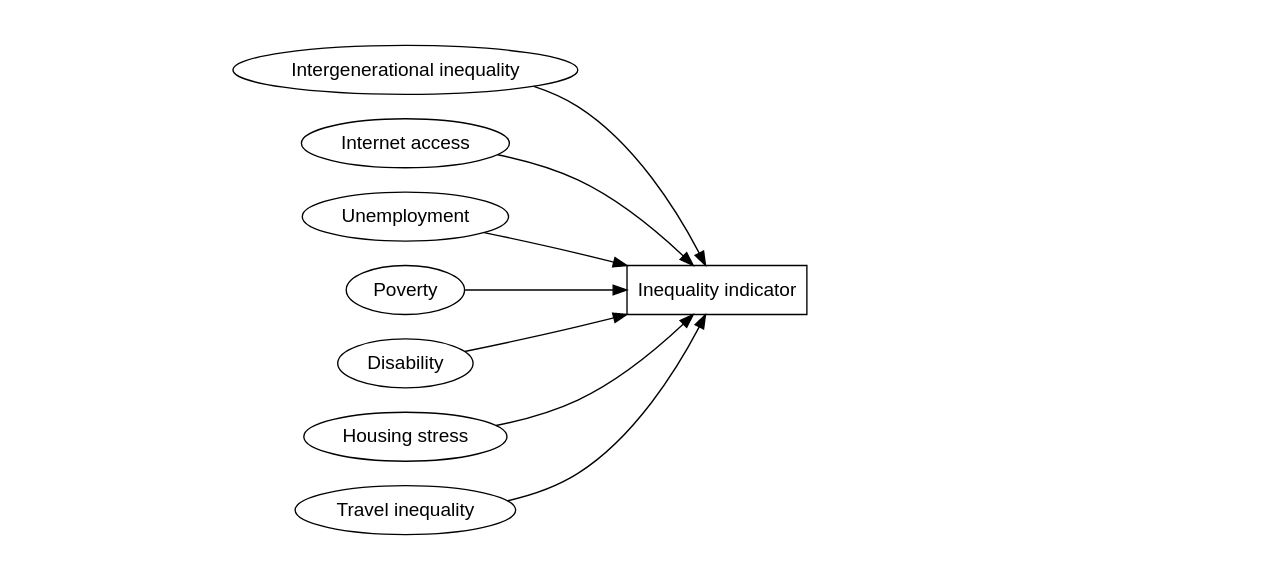
\includegraphics{Model-docs_files/figure-latex/unnamed-chunk-8-1.png}

Data are available at \url{https://github.com/pelagikat/Local-SDGs-systems-model}

\begin{center}\rule{0.5\linewidth}{0.5pt}\end{center}

\hypertarget{equations-7}{%
\section{\texorpdfstring{\emph{Equations}}{Equations}}\label{equations-7}}

\hypertarget{disability-fraction}{%
\subsection{disability fraction}\label{disability-fraction}}

Type: Constant\\
Formula: 0.177\\
Units: Dmnl\\
Assumptions: Data obtained from \href{https://www.abs.gov.au/statistics/health/disability/disability-ageing-and-carers-australia-summary-findings/2018}{ABS: Percentage of population who have a disability}

\hypertarget{households-without-internet-access-fraction}{%
\subsection{households without internet access fraction}\label{households-without-internet-access-fraction}}

Type: Auxiliary\\
Formula: 1-households with internet access fraction\\
Units: Dmnl\\
Assumptions: 1 minus the fraction of those with internet access (from Telecommunications)

\hypertarget{income-distribution-by-income-cohort}{%
\subsection{income distribution by income cohort}\label{income-distribution-by-income-cohort}}

Type: Auxiliary
Formula: sum(income distribution fractions by income cohort and gender)\\
Units: Dmnl\\
Assumptions: This variable is split (subscripted) across 15 income cohorts (negative, nil, \$1-\$149, \$150-\$299, \$300-\$399, \$400-\$499, \$500-\$649, \$650-\$799, \$800-\$999, \$1,000-\$1,249, \$1,250-\$1,499, \$1,250-\$1,499, \$1,750-\$1,999, \$2,000-\$2,999, \$3,000 or more) and summed over the two gender categories

\hypertarget{income-distribution-fractions-by-income-cohort-and-gender}{%
\subsection{income distribution fractions by income cohort and gender}\label{income-distribution-fractions-by-income-cohort-and-gender}}

Type: Constant\\
Formula: {[}Negative; M,F{]} = 0.006, 0.0022\\
{[}Nil; M,F{]} = 0.0105, 0.009\\
{[}``\$1-\$149''; M,F{]} = 0.0224, 0.0269\\
{[}``\$150-\$299''; M,F{]} = 0.0284, 0.0396\\
{[}``\$300-\$399''; M,F{]} = 0.0366, 0.0403\\
{[}``\$400-\$499''; M,F{]} = 0.0448, 0.0612\\
{[}``\$500-\$649''; M,F{]} = 0.0523, 0.0717\\
{[}``\$650-\$799''; M,F{]} = 0.0605, 0.0695\\
{[}``\$800-\$999''; M,F{]} = 0.0859, 0.0471\\
{[}``\$1,000-\$1,249''; M,F{]} = 0.0799, 0.0381\\
{[}``\$1,250-\$1,499''; M,F{]} = 0.0276, 0.0224\\
{[}``\$1,500-\$1,749''; M,F{]} = 0.0246, 0.0261\\
{[}``\$1,750-\$1,999''; M,F{]} = 0.0202, 0.003\\
{[}``\$2,000-\$2,999''; M,F{]} = 0.0194, 0.0105\\
{[}``\$3,000 or more''; M,F{]} = 0.0112, 0.0075\\
Units: Dmnl\\
Assumptions: Data from 2016 census, for weekly income. Disaggregated by gender - ABS only uses male and female for gender so is not comprehensive. Formulas above list {[}male, female{]}. See Github for data.

\hypertarget{inequality-indicator}{%
\subsection{inequality indicator}\label{inequality-indicator}}

Type: Auxiliary\\
Formula: (disability fraction + households without internet access fraction + normalised intergenerational inequality youth at risk +normalised poverty line + normalised travel inequality + normalised unemployed
+ normalised housing stress) / 7\\
Units: Dmnl\\
Assumptions: Arithmetic mean of normalised input variables

\hypertarget{intergenerational-risk-factor}{%
\subsection{intergenerational risk factor}\label{intergenerational-risk-factor}}

Type: Constant\\
Formula: 1.8\\
Units: structure/people\\
Assumptions: \citet{cobb-clarke_intergenerational_2017} estimate it is 1.8 times more likely for children of parents receiving long-term welfare to receive welfare themselves

\hypertarget{normalised-housing-stress}{%
\subsection{normalised housing stress}\label{normalised-housing-stress}}

Type: Auxiliary\\
Formula: (number of households under mortgage stress + number of households under rent stress) / Residential Housing\\
Units: Dmnl\\
Assumptions: Normalisation by number of residential households

\hypertarget{normalised-intergenerational-inequality-youth-at-risk}{%
\subsection{normalised intergenerational inequality youth at risk}\label{normalised-intergenerational-inequality-youth-at-risk}}

Type: Auxiliary\\
Formula: number of young people at risk for intergenerational inequality / ``0-14''\\
Units: Dmnl\\
Assumptions: Normalisation by 0-14 age cohort population

\hypertarget{normalised-poverty-line}{%
\subsection{normalised poverty line}\label{normalised-poverty-line}}

Type: Auxiliary\\
Formula: sum of people below poverty line / total population\\
Units: Dmnl\\
Assumptions: Normalisation by total population

\hypertarget{normalised-travel-inequality}{%
\subsection{normalised travel inequality}\label{normalised-travel-inequality}}

Type: Auxiliary\\
Formula: 1- (bus frequency / bus frequency required for travel equity)\\
Units: Dmnl\\
Assumptions: Normalisation by bus frequency and subtract result from 1 to obtain inequality instead of equity.

\hypertarget{normalised-unemployed}{%
\subsection{normalised unemployed}\label{normalised-unemployed}}

Type: Auxiliary\\
Formula: (number of unemployed people / total population) * normalised unemployed unit conversion\\
Units: Dmnl\\
Assumptions: normalisation by total population

\hypertarget{normalised-unemployed-unit-conversion}{%
\subsection{normalised unemployed unit conversion}\label{normalised-unemployed-unit-conversion}}

Type: Auxiliary\\
Formula: 1\\
Units: Year*people/job\\
Assumptions: Unit conversion to force all input units to dimensionless

\hypertarget{number-labour-force-in-income-bracket}{%
\subsection{number labour force in income bracket}\label{number-labour-force-in-income-bracket}}

Type: Auxiliary\\
Formula: INTEGER ( income distribution fractions by income cohort and gender * labour force)\\
Units: people\\
Assumptions: Summed over all income cohorts and genders

\hypertarget{number-of-unemployed-people}{%
\subsection{number of unemployed people}\label{number-of-unemployed-people}}

Type: Auxiliary\\
Formula: ``unemployment (agriculture)'' + ``unemployment (other)'' + ``unemployment (tourism)''\\
Units: job/Year\\
Assumptions:

\hypertarget{number-of-young-people-at-risk-for-intergenerational-inequality}{%
\subsection{number of young people at risk for intergenerational inequality}\label{number-of-young-people-at-risk-for-intergenerational-inequality}}

Type: Auxiliary\\
Formula: intergenerational risk factor * ``0-14'' * (sum of people below poverty line / Residential Housing)\\
Units: people\\
Assumptions: Multiply risk factor by proportion of total households below poverty line by youth cohort

\hypertarget{number-people-below-poverty-line}{%
\subsection{number people below poverty line}\label{number-people-below-poverty-line}}

Type: Auxiliary\\
Formula: number labour force in income bracket\\
Units: people\\
Assumptions: Poverty line is below first quartile (\$0 - \$399). This is in line with the ACOSS figure of \$457 (\citet{acoss_poverty_2020}). Excludes income cohorts above \$300-\$399.

\hypertarget{sum-of-people-below-poverty-line}{%
\subsection{sum of people below poverty line}\label{sum-of-people-below-poverty-line}}

Type: Auxiliary\\
Formula: sum ( number people below poverty line {[}poverty line ss!,Gender!{]} )\\
Units: people\\
Assumptions: Summed over income cohorts from Negative to \$300-\$399 and genders

\hypertarget{health-and-wellbeing-component}{%
\chapter{Health and Wellbeing component}\label{health-and-wellbeing-component}}

\hypertarget{problem-definition-8}{%
\section{\texorpdfstring{\emph{Problem definition}}{Problem definition}}\label{problem-definition-8}}

\begin{enumerate}
\def\labelenumi{\arabic{enumi}.}
\tightlist
\item
  Being in a regional area, Forrest does not have local access to healthcare services (closest hospital is Colac).
\end{enumerate}

\emph{Dynamic hypothesis:}
Living in regional areas impacts life expectancy.

\begin{enumerate}
\def\labelenumi{\arabic{enumi}.}
\setcounter{enumi}{1}
\tightlist
\item
  Potential disease burden in Forrest has been estimated to be approximately 80-90,000 times greater than the WHO target because of failing septic systems in Forrest.
\end{enumerate}

\emph{Dynamic hypothesis:}
Building new wastewater infrastructure will reduce disease burden

\begin{enumerate}
\def\labelenumi{\arabic{enumi}.}
\setcounter{enumi}{2}
\tightlist
\item
  Climate change and bushfire are risks to the local environment and population.
\end{enumerate}

\emph{Dynamic hypothesis:}
People like to live in Forrest because the local bush has a positive effect on wellbeing but there is a trade-off from bushfire risk

\begin{enumerate}
\def\labelenumi{\arabic{enumi}.}
\setcounter{enumi}{3}
\tightlist
\item
  There is a wide income distribution in Forrest, with a larger proportion of people in lower income brackets compared to the state.
\end{enumerate}

\emph{Dynamic hypothesis:}
People experiencing income inequality have poorer health outcomes (social gradient of health)

\hypertarget{system-conceptualisation-4}{%
\section{\texorpdfstring{\emph{System conceptualisation}}{System conceptualisation}}\label{system-conceptualisation-4}}

This component was inspired by the work of \citet{homer_system_2006}, and seeks to model local scale population health contributors. The community clearly identified positive and negative impacts on health and wellbeing, many of which are modelled in other components in the local SDG systems model.

\hypertarget{conceptual-model-6}{%
\subsection{Conceptual model}\label{conceptual-model-6}}

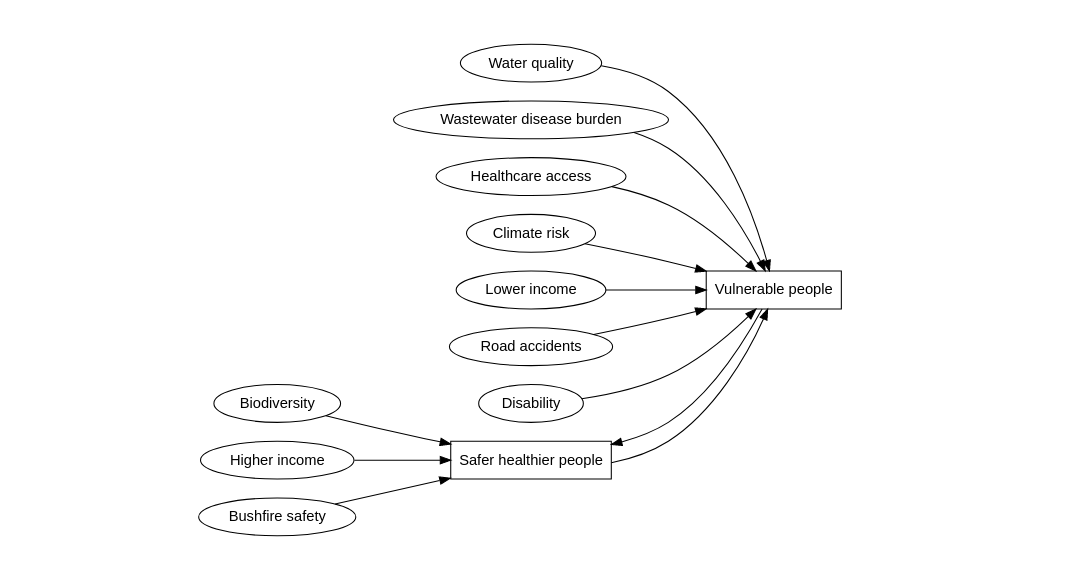
\includegraphics{Model-docs_files/figure-latex/unnamed-chunk-9-1.png}

\hypertarget{model-formulation-4}{%
\section{\texorpdfstring{\emph{Model formulation}}{Model formulation}}\label{model-formulation-4}}

Following the model in Figure 3 of \citet{homer_system_2006}, this component models ``Safer healthier people'' and ``Vulnerable people'' as stocks, and these form a cycle with flow variables. The various different health impacts (normalised where required) are multiplied together in the flow variables and this creates the dynamics of the model component.

\hypertarget{data-sources-6}{%
\section{Data sources}\label{data-sources-6}}

Data are available at \url{https://github.com/pelagikat/Local-SDGs-systems-model}

Data was obtained from the \href{https://discover.data.vic.gov.au/dataset/crash-stats-data-extract}{Victorian Government DATA VIC} for road accident statistics.

Census data for Forrest available \href{https://www.abs.gov.au/websitedbs/D3310114.nsf/Home/2016\%20QuickStats}{here.} Data for Forrest as a distinct location is only available for 2006, 2011 and 2016 censuses.

\hypertarget{abbreviations-1}{%
\section{Abbreviations}\label{abbreviations-1}}

GTOC = Gateway to the Otways Centre, a Bushfire Safer Place\\
WHO = World Health Organisation\\
WW = Wastewater, new local wastewater infrastructure

\begin{center}\rule{0.5\linewidth}{0.5pt}\end{center}

\hypertarget{equations-8}{%
\section{\texorpdfstring{\emph{Equations}}{Equations}}\label{equations-8}}

\hypertarget{accident-coefficient}{%
\subsection{accident coefficient}\label{accident-coefficient}}

Type: Constant\\
Formula: -19.25\\
Units: people\\
Assumptions: Calibrated against road accident data. See Github for data.

\hypertarget{becoming-safer-and-healthier}{%
\subsection{Becoming safer and healthier}\label{becoming-safer-and-healthier}}

Type: Auxiliary\\
Formula: (increasing bushfire safety from GTOC * ( biodiversity impact on health (middle and high income population / total population) * total population) / Time)\\
Units: people/Year\\
Assumptions:

\hypertarget{becoming-vulnerable}{%
\subsection{Becoming vulnerable}\label{becoming-vulnerable}}

Type: Auxiliary\\
Formula: (( climate risk * disability fraction * water quality * disease from wastewater * excess disease burden from lowered healthcare access * (low income population / total population) * (road accidents / total population)) * total population) / Time\\
Units: people/Year\\
Assumptions:

\hypertarget{biodiversity-impact-on-health}{%
\subsection{biodiversity impact on health}\label{biodiversity-impact-on-health}}

Type: Auxiliary\\
Formula: Species richness / INIT species richness\\
Units: Dmnl\\
Assumptions: Current species richness as a proportion of the baseline species richness

\hypertarget{climate-risk}{%
\subsection{climate risk}\label{climate-risk}}

Type: Auxiliary\\
Formula: risk to health from bushfire * risk to health from increasing temperatures\\
Units: Dmnl\\
Assumptions: the main risks to health as a result of climate are bushfire and high temperature

\hypertarget{disease-burden-before-ww}{%
\subsection{disease burden before WW}\label{disease-burden-before-ww}}

Type: Constant\\
Formula: 0.1\\
Units: Year/person\\
Assumptions: Wastewater investigation report in Forrest (\citet{decentralised_water_consulting_forrest_2019}, p.~28) found that the existing disease burden was approximately \(1 \times 10^{-1}\) (or 0.1) Disability Adjusted Life Years (DALYs). Note the \citet{decentralised_water_consulting_forrest_2019} report calls this ``Level of Disease Protection'' instead of disease burden, and appears to incorrectly interpret Figure 12 in the text.

\hypertarget{disease-from-wastewater}{%
\subsection{disease from wastewater}\label{disease-from-wastewater}}

Type: Auxiliary\\
Formula: (IF THEN ELSE ( Wastewater availability \textgreater{} 0, WHO target disease burden / WHO target disease burden, disease burden before WW / WHO target disease burden))\\
Units: Dmnl\\
Assumptions: Effect of installing new wastewater infrastructure as a proportion of the WHO target.

\hypertarget{excess-disease-burden-from-lowered-healthcare-access}{%
\subsection{excess disease burden from lowered healthcare access}\label{excess-disease-burden-from-lowered-healthcare-access}}

Type: Constant\\
Formula: 1.103\\
Units: fraction\\
Assumptions: Forrest is classified as inner regional by the \href{https://www.health.gov.au/health-topics/health-workforce/health-workforce-classifications/rural-remote-and-metropolitan-area}{RRMA classification}. Inner regional areas have 10.3\% excess disease burden compared to major cities (percentage of total observed burden for the area) (\citet{australian_institute_of_health_and_welfare_australian_2019}, Table 8.5)

\hypertarget{high-income-population}{%
\subsection{high income population}\label{high-income-population}}

Type: Auxiliary\\
Formula: sum ( number labour force in income bracket{[}high income!,Gender!{]})\\
Units: people\\
Assumptions: Summed over income cohorts \$1,500 and above, and summed over gender

\hypertarget{increasing-bushfire-safety-from-gtoc}{%
\subsection{increasing bushfire safety from GTOC}\label{increasing-bushfire-safety-from-gtoc}}

Type: Auxiliary\\
Formula: IF THEN ELSE ( GTOC availability \textgreater{} 0, 1-bushfire risk fraction, 1)\\
Units: Dmnl\\
Assumptions: If GTOC has been built, its presence negates the risk from bushfire as it is a Bushfire Safer Place

\hypertarget{low-income-population}{%
\subsection{low income population}\label{low-income-population}}

Type: Auxiliary\\
Formula: sum ( number labour force in income bracket{[}low income!, Gender!{]})\\
Units: people\\
Assumptions: Summed over income cohorts from Negative to \$649, and summed over gender.

\hypertarget{middle-and-high-income-population}{%
\subsection{middle and high income population}\label{middle-and-high-income-population}}

Type: Auxiliary\\
Formula: high income population + middle income population\\
Units: people\\
Assumptions:

\hypertarget{middle-income-population}{%
\subsection{middle income population}\label{middle-income-population}}

Type: Auxiliary\\
Formula: sum ( number labour force in income bracket{[}mid income!,Gender!{]})\\
Units: people\\
Assumptions: Summed over income cohorts from \$650 - \$1,499, and summed over gender.

\hypertarget{population-initial}{%
\subsection{population initial}\label{population-initial}}

Type: Constant\\
Formula: 171\\
Units: people\\
Assumptions: From 2006 census data, population at start of simulation.

\hypertarget{risk-to-health-from-bushfire}{%
\subsection{risk to health from bushfire}\label{risk-to-health-from-bushfire}}

Type: Auxiliary\\
Formula: bushfire risk fraction\\
Units: Dmnl\\
Assumptions: A one-to-one mapping of bushfire risk fraction

\hypertarget{risk-to-health-from-increasing-temperatures}{%
\subsection{risk to health from increasing temperatures}\label{risk-to-health-from-increasing-temperatures}}

Type: Auxiliary\\
Formula: climate damage fraction\\
Units: Dmnl\\
Assumptions: A one-to-one mapping of climate damage fraction

\hypertarget{road-accidents}{%
\subsection{road accidents}\label{road-accidents}}

Type: Auxiliary\\
Formula: Road Quality * accident coefficient + 9.6\\
Units: people\\
Assumptions: Linear model calibrated in Vensim. Intercept is dataset mean.

\hypertarget{safer-healthier-people}{%
\subsection{Safer Healthier People}\label{safer-healthier-people}}

Type: Stock\\
Formula: INTEG (Becoming safer and healthier - Becoming vulnerable), INITIAL = population initial\\
Units: people\\
Assumptions: There are only two states of being in this model: Safer \& Healthier, or Vulnerable.

\hypertarget{vulnerable-people}{%
\subsection{Vulnerable People}\label{vulnerable-people}}

Type: Stock\\
Formula: INTEG (Becoming vulnerable - Becoming safer and healthier), INITIAL = 0)\\
Units: people\\
Assumptions: There are only two states of being in this model: Safer \& Healthier, or Vulnerable. Assume that all the population begin as Safer \& Healthier and as the simulation runs, may move to Vulnerable.

\hypertarget{water-quality}{%
\subsection{water quality}\label{water-quality}}

Type: Constant\\
Formula: 1\\
Units: Dmnl\\
Assumptions: This is a scenario variable. The baseline is zero (no effect).

\hypertarget{who-target-disease-burden}{%
\subsection{WHO target disease burden}\label{who-target-disease-burden}}

Type: Constant\\
Formula: 1e-05\\
Units: Year/person\\
Assumptions: Wastewater investigation report in Forrest (\citet{decentralised_water_consulting_forrest_2019}, p.~28) states that the World Health Organisation target disease burden from wastewater was approximately \(1 \times 10^{-5}\) Disability Adjusted Life Years (DALYs). Note the \citet{decentralised_water_consulting_forrest_2019} report calls this ``Level of Disease Protection'' instead of disease burden, and appears to incorrectly interpret Figure 12 in the text. The new wastewater infrastructure will meet this disease burden target.

\hypertarget{telecommunications-component}{%
\chapter{Telecommunications component}\label{telecommunications-component}}

\hypertarget{problem-definition-9}{%
\section{\texorpdfstring{\emph{Problem definition}}{Problem definition}}\label{problem-definition-9}}

The NBN has been rolled out in Forrest, but the service can be poor. NBN Fixed Wireless is known to suffer from congestion issues, and the distance to the fixed wireless tower can also affect internet speeds. The nearest tower to Forrest is in Barwon Downs, and towers have an effective range of 14kms, which can be disrupted by terrain (trees, mountains, etc.), and precipitation. There is also limited mobile reception throughout Forrest.

\emph{Dynamic hypothesis:} Poor internet and mobile phone service impacts establishment of new businesses and growth of existing ones. Improved internet access (fixed and mobile) would encourage new businesses which rely on connectivity, and better support the existing residents and businesses. It is also necessary for education and better health outcomes.

\hypertarget{system-conceptualisation-5}{%
\section{\texorpdfstring{\emph{System conceptualisation}}{System conceptualisation}}\label{system-conceptualisation-5}}

We are only considering Fixed Wireless NBN in our model. We wish to explore how internet demand, infrastructure (in the form of Fixed Wireless towers) and internet capacity interact in Forrest. There are a number of assumptions made on limited data for some of these variables as much of the information underlying the NBN is commercial-in-confidence.

\hypertarget{conceptual-model-7}{%
\subsection{Conceptual model}\label{conceptual-model-7}}

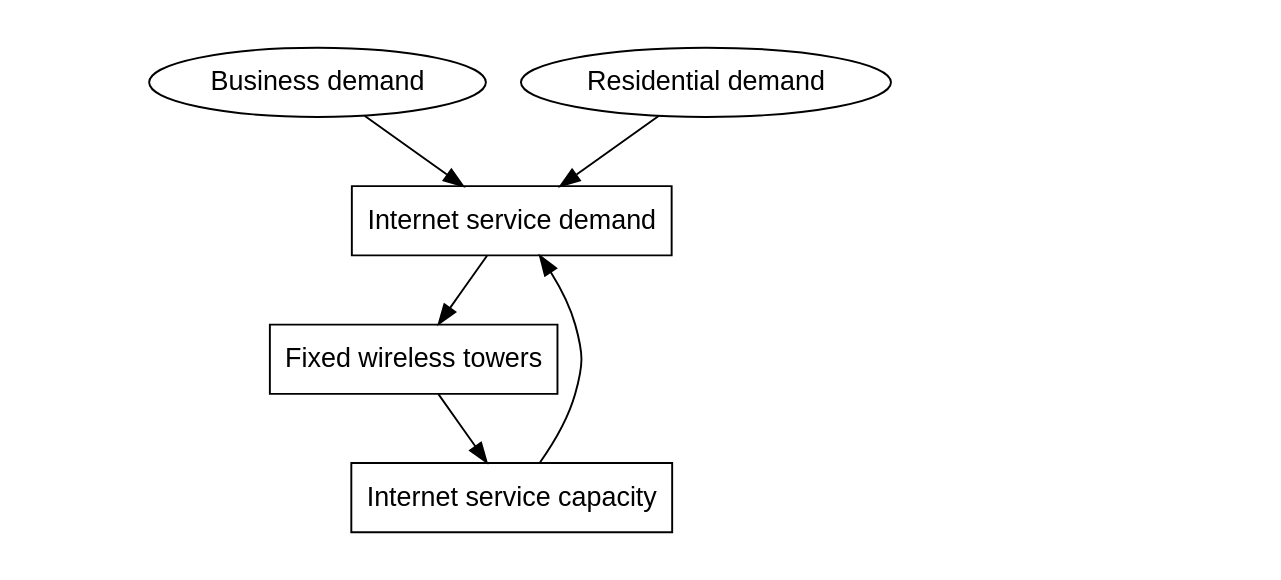
\includegraphics{Model-docs_files/figure-latex/unnamed-chunk-10-1.png}

\hypertarget{model-formulation-5}{%
\section{\texorpdfstring{\emph{Model formulation}}{Model formulation}}\label{model-formulation-5}}

There are three stocks with inflow rates forming the basis of the model: Internet Service Demand, Fixed Wireless Towers, and Internet Service Capacity. Demand is influenced by business and residential internet demand. Capacity is influenced by demand, user limits and speeds per connection. Fixed wireless towers is influenced by oversubscription of the existing infrastructure (i.e.~how far the capacity exceeds the user limit). We have not modelled infrastructure funding in this case, as NBN Co is supposed to roll out upgrades according to need (although this is intermittent currently), and it is funded by the Federal Government.

\hypertarget{data-sources-7}{%
\section{Data sources}\label{data-sources-7}}

Data are available at \url{https://github.com/pelagikat/Local-SDGs-systems-model} (Economic data is used in this component)

Census data for Forrest available \href{https://www.abs.gov.au/websitedbs/D3310114.nsf/Home/2016\%20QuickStats}{here.} Data for Forrest as a distinct location is only available for 2006, 2011 and 2016 censuses.

Data was obtained from Australian Bureau of Statistics
\href{https://www.abs.gov.au/statistics/economy/business-indicators/counts-australian-businesses-including-entries-and-exits/latest-release}{Counts of Australian Businesses}
and \href{https://www.abs.gov.au/websitedbs/censushome.nsf/home/tablebuilder}{Census Table Builder}

\begin{center}\rule{0.5\linewidth}{0.5pt}\end{center}

\hypertarget{equations-9}{%
\section{\texorpdfstring{\emph{Equations}}{Equations}}\label{equations-9}}

\hypertarget{business-internet-demand}{%
\subsection{business internet demand}\label{business-internet-demand}}

Type: Auxiliary\\
Formula: ``number of businesses (agriculture)'' + ``number of businesses (other)'' + ``number of businesses (tourism)''\\
Units: structure\\
Assumptions: Assume that all businesses require a connection to the internet

\hypertarget{demand-per-location}{%
\subsection{demand per location}\label{demand-per-location}}

Type: Constant\\
Formula: 1\\
Units: connections/structure\\
Assumptions: 1 connections per location

\hypertarget{fixed-wireless-tower-investment-rate}{%
\subsection{Fixed wireless tower investment rate}\label{fixed-wireless-tower-investment-rate}}

Type: Auxiliary (rate)\\
Formula: tower oversubscription factor / Time\\
Units: tower/Year\\
Assumptions:

\hypertarget{fixed-wireless-towers}{%
\subsection{Fixed Wireless Towers}\label{fixed-wireless-towers}}

Type: Stock\\
Formula: INTEG ( INTEGER(Fixed wireless tower investment rate)), INITIAL = INIT number of towers\\
Units: tower\\
Assumptions:

\hypertarget{fixed-wireless-user-limit}{%
\subsection{fixed wireless user limit}\label{fixed-wireless-user-limit}}

Type: Constant\\
Formula: 60\\
Units: connections/tower\\
Assumptions: This value was difficult to ascertain, however \href{https://www.itnews.com.au/news/nbn-co-cuts-average-number-of-users-per-wireless-cell-to-19-559707}{this article} quoted NBN Co saying they had reduced users from historical levels of 60 per cell to an average of 19. Based upon that, we assume 60 connections is higher than acceptable and have set that as the maximum value.

\hypertarget{households-with-internet-access-fraction}{%
\subsection{households with internet access fraction}\label{households-with-internet-access-fraction}}

Type: Constant\\
Formula: 0.77\\
Units: fraction\\
Assumptions: From ABS 2016 census data: 77\% of households accessed the internet from their home

\hypertarget{init-nbn-connections}{%
\subsection{INIT NBN connections}\label{init-nbn-connections}}

Type: Constant\\
Formula: 114 + 27\\
Units: connections\\
Assumptions: 77\% of 148 dwellings (from 2016 ABS Census data) plus 27 businesses (from 2020 ABS counts of businesses). See Github for data.

\hypertarget{init-number-of-towers}{%
\subsection{INIT number of towers}\label{init-number-of-towers}}

Type: Constant\\
Formula: 1\\
Units: tower\\
Assumptions: There is one fixed wireless tower in Forrest

\hypertarget{internet-capacity-demand}{%
\subsection{internet capacity demand}\label{internet-capacity-demand}}

Type: Auxiliary\\
Formula: Internet Service Demand * maximum speed per connection / Fixed Wireless Towers\\
Units: Mbps * connection/tower\\
Assumptions: This is a variable which represents the total amount of traffic demand as a proportion of number of towers.

\hypertarget{internet-capacity-discrepancy}{%
\subsection{internet capacity discrepancy}\label{internet-capacity-discrepancy}}

Type: Auxiliary\\
Formula: internet capacity demand-Internet Service Capacity\\
Units: Mbps*connection/tower\\
Assumptions: This is the discrepancy between capacity demand and capacity actual.

\hypertarget{internet-service-capacity}{%
\subsection{Internet Service Capacity}\label{internet-service-capacity}}

Type: Stock\\
Formula: INTEG ( Internet service capacity rate), INITIAL = maximum speed per connection * fixed wireless user limit\\
Units: Mbps * connections/tower\\
Assumptions: The initial value is the maximum available capacity

\hypertarget{internet-service-capacity-rate}{%
\subsection{Internet service capacity rate}\label{internet-service-capacity-rate}}

Type: Auxiliary\\
Formula: IF THEN ELSE ( tower oversubscription factor \textless= Fixed Wireless Towers, internet capacity discrepancy / Time, (fixed wireless user limit * maximum speed per connection) / Time)\\
Units: Mbps * connection /(Year * tower)\\
Assumptions: If the tower oversubscription factor is less than the number of towers (i.e., there are enough towers), then the discrepancy structure will be valid. However, if there are not enough towers to meet demand, then the capacity rate will stay at its max level, which is the user limit * max speed per connection.

\hypertarget{internet-service-demand}{%
\subsection{Internet Service Demand}\label{internet-service-demand}}

Type: Stock\\
Formula: INTEG ( Internet service demand rate ), INITIAL = INIT NBN connections\\
Units: connections\\
Assumptions:

\hypertarget{internet-service-demand-rate}{%
\subsection{Internet service demand rate}\label{internet-service-demand-rate}}

Type: Auxiliary (rate)\\
Formula: (business internet demand + residential internet demand) * demand per location / Time\\
Units: connections/Year\\
Assumptions: Assume that all businesses require a connection to the internet

\hypertarget{internet-service-performance}{%
\subsection{internet service performance}\label{internet-service-performance}}

Type: Auxiliary\\
Formula: Internet Service Capacity / Internet Service Demand\\
Units: Mbps/tower\\
Assumptions: This is the equivalent of a supply/demand ratio

\hypertarget{max-number-of-premises-to-connect-to-the-internet}{%
\subsection{max number of premises to connect to the internet}\label{max-number-of-premises-to-connect-to-the-internet}}

Type: Constant\\
Formula: Residential Housing + Tourism Housing\\
Units: structure\\
Assumptions:

\hypertarget{maximum-speed-per-connection}{%
\subsection{maximum speed per connection}\label{maximum-speed-per-connection}}

Type: Constant\\
Formula: 75\\
Units: Mbps\\
Assumptions: Fixed wireless has a maximum plan speed of 75Mbps

\hypertarget{residential-internet-demand}{%
\subsection{residential internet demand}\label{residential-internet-demand}}

Type: Auxiliary\\
Formula: max number of premises to connect to the internet * households with internet access fraction\\
Units: structure\\
Assumptions:

\hypertarget{tower-build-delay-time}{%
\subsection{tower build delay time}\label{tower-build-delay-time}}

Type: Constant\\
Formula: 2\\
Units: Year\\
Assumptions: Assume it takes two years to build

\hypertarget{tower-investment-responsiveness}{%
\subsection{tower investment responsiveness}\label{tower-investment-responsiveness}}

Type: Constant\\
Formula: 0\\
Units: Dmnl\\
Assumptions: This variable represents whether or not a new tower is built when it is oversubscribed. Currently a binary (yes/no; 0/1) but can be modified to be an investment delay

\hypertarget{tower-oversubscription-factor}{%
\subsection{tower oversubscription factor}\label{tower-oversubscription-factor}}

Type: Auxiliary\\
Formula: INIT number of towers + (Internet Service Demand / fixed wireless user limit) - Fixed Wireless Towers\\
Units: tower\\
Assumptions: Desired state of system (Initial number of towers plus the number mandated by the demand)

\hypertarget{infrastructure-component}{%
\chapter{Infrastructure component}\label{infrastructure-component}}

The Forrest community have four major infrastructure projects currently in train which they have identified as being important for the future development and growth of Forrest. There is one additional project which is as important for the community but not reliant on outside intervention.

\hypertarget{problem-definition-10}{%
\section{\texorpdfstring{\emph{Problem definition}}{Problem definition}}\label{problem-definition-10}}

\begin{enumerate}
\def\labelenumi{\arabic{enumi}.}
\tightlist
\item
  In the past, on-site septic systems were adequate for a town the size of Forrest, which did not have many visitors. With the change to a tourism economy, there are many more people that come to town, particularly for events, and the now ageing septic infrastructure requires upgrading. The limits of septic infrastructure for waste are hindering attempts to increase housing in the town. Studies have been undertaken by Barwon Water to upgrade wastewater infrastructure but there has been no progress, partly due to funding issues. The current option on the table expects the community to contribute, which may delay or entirely derail the development.
\end{enumerate}

\emph{Dynamic hypothesis:}
Ageing septic systems that don't meet current safety standards are no longer adequate and new infrastructure is urgently needed. This affects the local environment and biodiversity, the local economy (by limiting tourism), health of local residents, and additional development in the town.

\begin{enumerate}
\def\labelenumi{\arabic{enumi}.}
\setcounter{enumi}{1}
\tightlist
\item
  The Forrest MTB Trails were first opened in 2005, encompassing over 60km of trails. A proposal was released in December 2019 to increase the MTB trail network by approximately 38kms, including restructuring the existing trails and creating a new Trail Head. This plan is aimed to revitalise mountain bike tourism and re-establish Forrest as a nationally significant mountain bike destination.
\end{enumerate}

\emph{Dynamic hypothesis:}
Mountain bike trails in Forrest are already a major tourism drawcard but upgrades to the trail network would encourage more visitation to the town. This is a benefit to the tourism economy but issues still remain around accommodation (i.e.~housing supply) and wastewater.

\begin{enumerate}
\def\labelenumi{\arabic{enumi}.}
\setcounter{enumi}{2}
\tightlist
\item
  The Forrest Common is a piece of public land which could be put to better use for the community. After several years of consultation with Colac Otway Shire, a plan has been approved but it is beyond the ability of Council to fund.
\end{enumerate}

\emph{Dynamic hypothesis:}
A revamped Forrest Common would benefit tourism and in-migration of families (due to new play equipment).

\begin{enumerate}
\def\labelenumi{\arabic{enumi}.}
\setcounter{enumi}{3}
\tightlist
\item
  The community identified that a bushfire safer place is necessary for the community, and that one of the DELWP parcels of land could be used to achieve this. A feasibility study and preliminary plans have been completed, but funding needs to be found to build it.
\end{enumerate}

\emph{Dynamic hypothesis:}
If funding can be obtained for the Gateway to The Otways Centre, this would have a positive impact on community health and wellbeing in the event of a bushfire and potentially prevent loss of life.

\hypertarget{system-conceptualisation-6}{%
\section{\texorpdfstring{\emph{System conceptualisation}}{System conceptualisation}}\label{system-conceptualisation-6}}

The life cycle of an infrastructure project is focused on three stages: acquiring the funding, building the infrastructure, and completion of the project. Accordingly, we have developed our system around these three stages.

\hypertarget{conceptual-model-8}{%
\subsection{Conceptual model}\label{conceptual-model-8}}

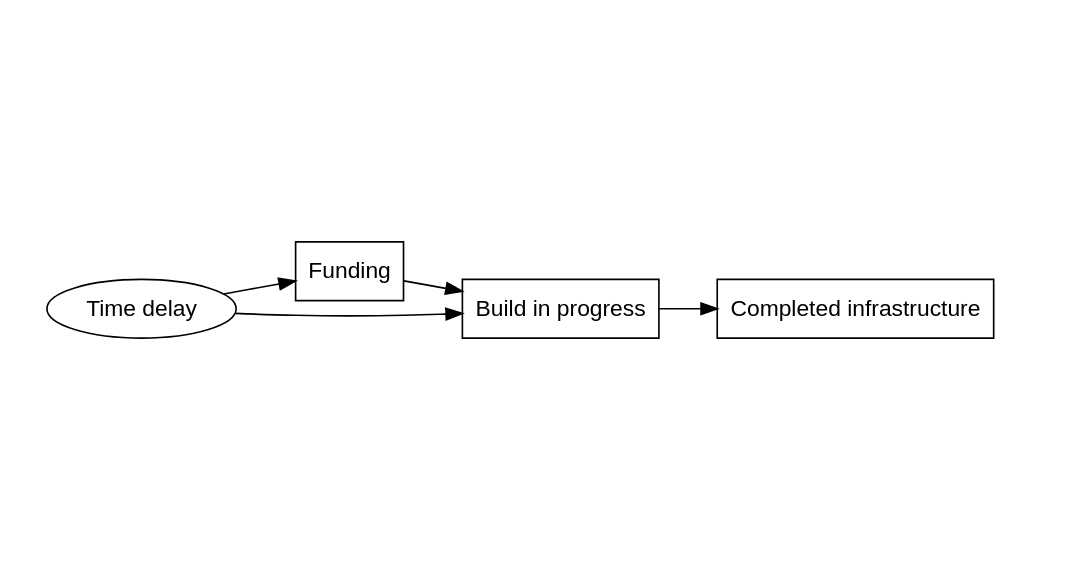
\includegraphics{Model-docs_files/figure-latex/unnamed-chunk-11-1.png}

\hypertarget{model-formulation-6}{%
\section{\texorpdfstring{\emph{Model formulation}}{Model formulation}}\label{model-formulation-6}}

We have defined the Funding, Build-in-Progress and Completion stages of infrastructure projects as stocks in the model. We have incorporated delays through the process for funding, build delay and build time. The crucial information which is required for other model components is the time at which the build is complete and the infrastructure is ready for use.

As there are five infrastructure projects and the process is the same for each, the five projects have been subscripted into model structure; that is, five different versions (subscripts) exist in the one model structure.

\hypertarget{abbreviations-used}{%
\subsection{Abbreviations used:}\label{abbreviations-used}}

CFA = Country Fire Authority (regional fire service)\\
GTOC = Gateway to the Otways Centre (bushfire safer place)\\
MTB = Mountain Bike (e.g., MTB Trails = Mountain Bike Trails)

\begin{center}\rule{0.5\linewidth}{0.5pt}\end{center}

\hypertarget{equations-10}{%
\section{\texorpdfstring{\emph{Equations}}{Equations}}\label{equations-10}}

\hypertarget{asset-component-discrepancy}{%
\subsection{asset component discrepancy}\label{asset-component-discrepancy}}

Type: Auxiliary\\
Formula: total number of asset components - Completed Infrastructure Item\\
Units: asset component\\
Assumptions: This variable is split (subscripted) across the 5 infrastructure projects.

\hypertarget{build-delay}{%
\subsection{build delay}\label{build-delay}}

Type: Constant\\
Formula: {[}Forrest Common{]} = 0.5\\
{[}GTOC{]} = 1\\
{[}MTB Trails{]} = 1\\
{[}Wastewater{]} = 2\\
{[}CFA Truck{]} = 0.5\\
Units: Year
Assumptions: Arbitrary values; can be used for scenarios if needed.

\hypertarget{build-time}{%
\subsection{build time}\label{build-time}}

Type: Constant\\
Formula: {[}Forrest Common{]} = 0.5\\
{[}GTOC{]} = 2\\
{[}MTB Trails{]} = 1\\
{[}Wastewater{]} = 3\\
{[}CFA Truck{]} = 0.25\\
Units: Year\\
Assumptions: Arbitrary values; can be used for scenarios if needed.

\hypertarget{cfa-truck-availability}{%
\subsection{CFA Truck availability}\label{cfa-truck-availability}}

Type: Auxiliary\\
Formula: IF THEN ELSE (time at which infrastructure item is complete{[}CFA Truck{]} \textgreater{} 0, STEP(1, (Current time + time at which infrastructure item is complete {[}CFA Truck{]})) , 0 )\\
Units: Year\\
Assumptions: The time from which the infrastructure is complete and can begin having an effect on other variables

\hypertarget{completed-infrastructure-item}{%
\subsection{Completed Infrastructure Item}\label{completed-infrastructure-item}}

Type: Stock\\
Formula: INTEG (Infrastructure completion rate), INITIAL = 0)\\
Units: asset component\\
Assumptions: This variable is split (subscripted) across the 5 infrastructure projects.

\hypertarget{cost-per-asset-component}{%
\subsection{cost per asset component}\label{cost-per-asset-component}}

Type: Constant\\
Formula: {[}Forrest Common{]} = 1.7e+06 / 10\\
{[}GTOC{]} = ( 1.2e+07) / 10\\
{[}MTB Trails{]} = 4.55e+06 / 10\\
{[}Wastewater{]} = 1.01e+07 / 10\\
{[}CFA Truck{]} = 210000 / 10\\
Units: dollar/asset component\\
Assumptions: Total cost of project divided by 10

\hypertarget{current-time-1}{%
\subsection{Current time}\label{current-time-1}}

Type: Constant\\
Formula: 2021\\
Units: Year\\
Assumptions: Reference year to compare to project completion times.

\hypertarget{forrest-common-availability}{%
\subsection{Forrest Common availability}\label{forrest-common-availability}}

Type: Auxiliary\\
Formula: IF THEN ELSE ( time at which infrastructure item is complete {[}Forrest Common{]} \textgreater0, STEP(1, (Current time + time at which infrastructure item is complete{[}Forrest Common{]})) , 0 )\\
Units: Year\\
Assumptions: The time from which the infrastructure is complete and can begin having an effect on other variables

\hypertarget{funding-duration}{%
\subsection{funding duration}\label{funding-duration}}

Type: Constant\\
Formula: {[}Forrest Common{]} = 1\\
{[}GTOC{]} = 2\\
{[}MTB Trails{]} = 1\\
{[}Wastewater{]} = 3\\
{[}CFA Truck{]} = 1\\
Units: Year\\
Assumptions: Arbitrary values; can be used for scenarios if needed.

\hypertarget{funding-lag}{%
\subsection{funding lag}\label{funding-lag}}

Type: Constant\\
Formula: {[}Forrest Common{]} = 2\\
{[}GTOC{]} = 5\\
{[}MTB Trails{]} = 0.5\\
{[}Wastewater{]} = 2\\
{[}CFA Truck{]} = 1\\
Units: Year\\
Assumptions: Arbitrary values; can be used for scenarios if needed.

\hypertarget{funding-scenario}{%
\subsection{funding scenario}\label{funding-scenario}}

Type: Constant\\
Formula: {[}Forrest Common{]} = 0\\
{[}GTOC{]} = 0\\
{[}MTB Trails{]} = 1\\
{[}Wastewater{]} = 0\\
{[}CFA Truck{]} = 0\\
Units: Dmnl\\
Assumptions: This is a `switch' variable (0 = off, 1 = on)

\hypertarget{gtoc-availability}{%
\subsection{GTOC availability}\label{gtoc-availability}}

Type: Auxiliary\\
Formula: IF THEN ELSE ( time at which infrastructure item is complete{[}GTOC{]} \textgreater{} 0, STEP (1, (Current time + time at which infrastructure item is complete{[}GTOC{]})) , 0 )\\
Units: Year\\
Assumptions: The time from which the infrastructure is complete and can begin having an effect on other variables

\hypertarget{infrastructure-approved-funding}{%
\subsection{infrastructure approved funding}\label{infrastructure-approved-funding}}

Type: Auxiliary\\
Formula: {[}Forrest Common{]} = IF THEN ELSE ( funding scenario{[}Forrest Common{]} = 1, 1.7e+06, 0)\\
{[}GTOC{]} = IF THEN ELSE ( funding scenario{[}GTOC{]} = 1, 1.2e+07, 0)\\
{[}MTB Trails{]} = IF THEN ELSE ( funding scenario{[}MTB Trails{]} = 1, 4.55e+06, 0)\\
{[}Wastewater{]} = IF THEN ELSE ( funding scenario{[}Wastewater{]} = 1, 1.01e+07, 0)\\
{[}CFA Truck{]} = IF THEN ELSE ( funding scenario{[}CFA Truck{]} = 1, 21000, 0)
Units: dollar
Assumptions: These values are the funding estimates for each project. See The Forrest and District Plan for more information (\citet{szetey_forrest_2020})

\hypertarget{infrastructure-build-in-progress}{%
\subsection{Infrastructure Build In Progress}\label{infrastructure-build-in-progress}}

Type: Stock\\
Formula: INTEG (Infrastructure start rate - Infrastructure completion rate), INITIAL = 0)\\
Units: asset component\\
Assumptions: This variable is split (subscripted) across the 5 infrastructure projects.

\hypertarget{infrastructure-completion-rate}{%
\subsection{Infrastructure completion rate}\label{infrastructure-completion-rate}}

Type: Auxiliary\\
Formula: (asset component discrepancy) / build time\\
Units: asset component/Year\\
Assumptions: This variable is split (subscripted) across the 5 infrastructure projects.

\hypertarget{infrastructure-funding}{%
\subsection{Infrastructure Funding}\label{infrastructure-funding}}

Type: Stock\\
Formula: INTEG ( -Infrastructure funding allocation rate), INITIAL = infrastructure approved funding\\
Units: dollar\\
Assumptions: This variable is split (subscripted) across the 5 infrastructure projects.

\hypertarget{infrastructure-funding-allocation-rate}{%
\subsection{Infrastructure funding allocation rate}\label{infrastructure-funding-allocation-rate}}

Type: Auxiliary\\
Formula: Infrastructure Funding / funding duration\\
Units: dollar/Year\\
Assumptions: This variable is split (subscripted) across the 5 infrastructure projects.

\hypertarget{infrastructure-start-rate}{%
\subsection{Infrastructure start rate}\label{infrastructure-start-rate}}

Type: Auxiliary\\
Formula: DELAY1 ( Infrastructure funding allocation rate / cost per asset component, build delay + funding lag)\\
Units: asset component/Year\\
Assumptions: This variable is split (subscripted) across the 5 infrastructure projects.

\hypertarget{mtb-trails-improvements-availability}{%
\subsection{MTB trails improvements availability}\label{mtb-trails-improvements-availability}}

Type: Auxiliary\\
Formula: IF THEN ELSE ( time at which infrastructure item is complete{[}MTB Trails {]}\textgreater{} 0, STEP(1, (Current time + time at which infrastructure item is complete{[}MTB Trails{]})) , 0 )\\
Units: Year\\
Assumptions: The time from which the infrastructure is complete and can begin having an effect on other variables

\hypertarget{time-at-which-infrastructure-item-is-complete}{%
\subsection{time at which infrastructure item is complete}\label{time-at-which-infrastructure-item-is-complete}}

Type: Auxiliary\\
Formula: IF THEN ELSE(funding scenario \textgreater{} 0, build delay + build time + funding lag , 0 )\\
Units: Year\\
Assumptions: This variable is split (subscripted) across the 5 infrastructure projects.

\hypertarget{total-number-of-asset-components}{%
\subsection{total number of asset components}\label{total-number-of-asset-components}}

Type: Constant\\
Formula: 10\\
Units: asset component\\
Assumptions: Have arbitrarily assumed that each infrastructure project has 10 stages. This variable is split (subscripted) across the 5 infrastructure projects.

\hypertarget{wastewater-availability}{%
\subsection{Wastewater availability}\label{wastewater-availability}}

Type: Auxiliary\\
Formula: IF THEN ELSE ( time at which infrastructure item is complete{[}Wastewater{]} \textgreater{} 0, STEP(1, (Current time + time at which infrastructure item is complete{[}Wastewater{]})) , 0 )\\
Units: Year\\
Assumptions: The time from which the infrastructure is complete and can begin having an effect on other variables

\hypertarget{transport-component}{%
\chapter{Transport component}\label{transport-component}}

\hypertarget{problem-definition-11}{%
\section{\texorpdfstring{\emph{Problem definition}}{Problem definition}}\label{problem-definition-11}}

\begin{enumerate}
\def\labelenumi{\arabic{enumi}.}
\tightlist
\item
  Forrest lies on the route between Apollo Bay and Colac. It is a feeder route to tourism along the Great Ocean Road and the Great Otway National Park. Recent upgrades to the channel routes to Forrest make it easier for tourists to visit the area, and safer for residents to drive.
\end{enumerate}

\emph{Dynamic hypothesis:}
Forrest is midway between Colac and Apollo Bay, and the road between them is a key route to the tourism of the Great Ocean Road. It is important that these roads remain in excellent condition for safety of road users. Road deaths on rural roads far exceed those in metropolitan areas.

\begin{enumerate}
\def\labelenumi{\arabic{enumi}.}
\setcounter{enumi}{1}
\tightlist
\item
  There is one bus line that runs through Forrest, the Colac-Marengo route. This service runs only on Wednesdays and only once in each direction. There is a V-Line station in Birregurra, but apart from the once-weekly bus, there is no connecting service from Birregurra to Forrest, and there is no alignment of the bus timetable with the train timetable. This puts a severe limit on residents who may want to avoid driving, and for tourists who wish to visit that do not drive.
\end{enumerate}

\emph{Dynamic hypothesis:}
There is poor public transport service from Forrest to Colac or Birregurra. One service per week does not enable general uptake of public transport. This is also an inequality issue, as people of lower incomes may not be able to afford to own or use a car, and this also restricts mobility for those unable to drive, due to age or disability. More tourists may visit if there was better public transport access.

\hypertarget{system-conceptualisation-7}{%
\section{\texorpdfstring{\emph{System conceptualisation}}{System conceptualisation}}\label{system-conceptualisation-7}}

There are three main structures to the model of transport in Forrest. The first is road quality, the second is car use, and the third is modelling the dynamics of public transport, for which Forrest is only served by buses. Within the bus structure, we examine the current level of service, the potential level of service, and the service that would be required for there to be travel equity across the population. By travel equity, we mean that there are frequent enough bus services that people who are of lower income or reduced mobility would have as much mobility as someone with a car.

\hypertarget{conceptual-model-9}{%
\subsection{Conceptual model}\label{conceptual-model-9}}

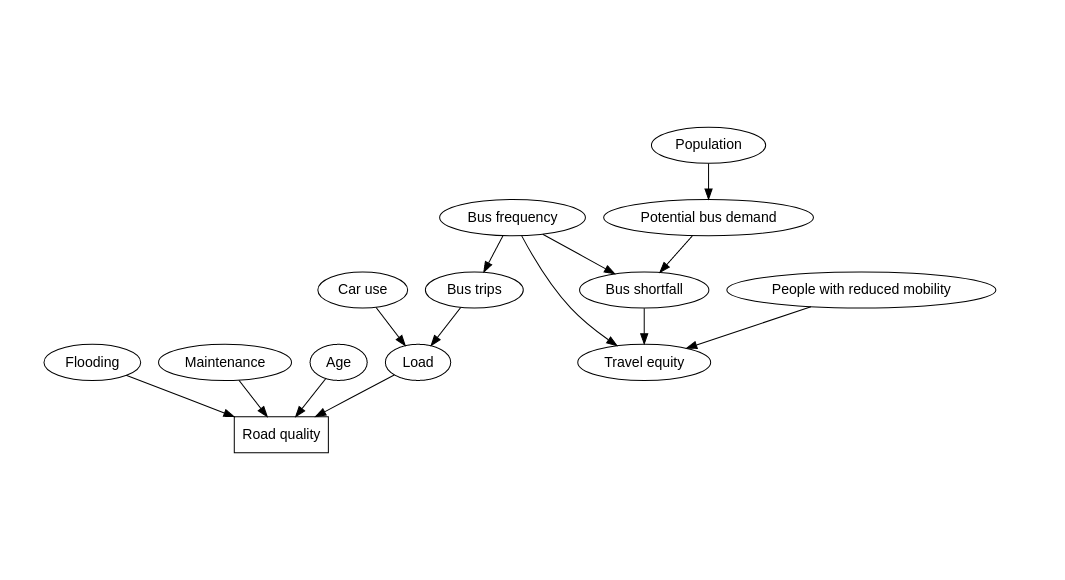
\includegraphics{Model-docs_files/figure-latex/unnamed-chunk-12-1.png}

\hypertarget{model-formulation-7}{%
\section{\texorpdfstring{\emph{Model formulation}}{Model formulation}}\label{model-formulation-7}}

The road quality structure was adapted from work by \citet{fallah-fini_measuring_2015}. We added flooding as a factor in road deterioration. The car use structure was built from data on the number of cars in Forrest and the number of car trips made each year. The bus demand structure developed from understanding how the current levels of service fell short, and examining how service levels would need to increase to meet potential demand. The travel equity structure then fed into this to calculate how demand would increase to serve those of reduced mobility.

\hypertarget{data-sources-8}{%
\section{Data sources}\label{data-sources-8}}

Australian Bureau of Statistics: \href{https://www.abs.gov.au/statistics/industry/tourism-and-transport/survey-motor-vehicle-use-australia/latest-release}{Car use in Australia}

Travel to work - ABS \href{https://quickstats.censusdata.abs.gov.au/census_services/getproduct/census/2016/quickstat/SSC20933}{Census data}

\begin{center}\rule{0.5\linewidth}{0.5pt}\end{center}

\hypertarget{equations-11}{%
\section{\texorpdfstring{\emph{Equations}}{Equations}}\label{equations-11}}

\hypertarget{age-of-pavement}{%
\subsection{age of pavement}\label{age-of-pavement}}

Type: Constant\\
Formula: 10\\
Units: Year\\
Assumptions: Assume 10 year old pavements at start of simulation. From \citet{fallah-fini_measuring_2015}.

\hypertarget{ageing-nonlinearity-factor}{%
\subsection{ageing nonlinearity factor}\label{ageing-nonlinearity-factor}}

Type: Constant\\
Formula: 1.42\\
Units: Dmnl\\
Assumptions: Exponent of function. From \citet{fallah-fini_measuring_2015}.

\hypertarget{allowable-number-of-load-cycles}{%
\subsection{allowable number of load cycles}\label{allowable-number-of-load-cycles}}

Type: Constant\\
Formula: 1e+08\\
Units: trip/Year\\
Assumptions: From \citet{fallah-fini_measuring_2015}

\hypertarget{annual-bus-capacity-discrepancy}{%
\subsection{annual bus capacity discrepancy}\label{annual-bus-capacity-discrepancy}}

Type: Auxiliary\\
Formula: annual potential bus demand - max annual capacity of bus route\\
Units: trip*people/Year\\
Assumptions:

\hypertarget{annual-potential-bus-demand}{%
\subsection{annual potential bus demand}\label{annual-potential-bus-demand}}

Type: Auxiliary\\
Formula: average number of bus trips per year * number people with ability to travel by bus\\
Units: trip*people/Year\\
Assumptions:

\hypertarget{annual-probability-of-flood-1}{%
\subsection{annual probability of flood}\label{annual-probability-of-flood-1}}

Type: Constant\\
Formula: 0.01\\
Units: Dmnl\\
Assumptions: Corangamite Catchment Management Authority \href{https://www.ccmaknowledgebase.vic.gov.au/flood/cb_pages/flood_mapping.php}{flood mapping portal} shows 1 in 100 year riverine flood extent (limited data)

\hypertarget{average-litres-of-petrol-per-100km}{%
\subsection{average litres of petrol per 100km}\label{average-litres-of-petrol-per-100km}}

Type: Constant\\
Formula: 11.1\\
Units: litre\\
Assumptions: \href{https://www.abs.gov.au/statistics/industry/tourism-and-transport/survey-motor-vehicle-use-australia/latest-release}{Source}

\hypertarget{average-number-of-bus-trips-per-year}{%
\subsection{average number of bus trips per year}\label{average-number-of-bus-trips-per-year}}

Type: Constant\\
Formula: 156\\
Units: trip/Year\\
Assumptions: 3 x return trips per week per person = 156 trips per person

\hypertarget{average-trip-distance}{%
\subsection{average trip distance}\label{average-trip-distance}}

Type: Constant\\
Formula: 19\\
Units: Km\\
Assumptions: Data derived from census data: \emph{travel to work days}

\hypertarget{bus-capacity}{%
\subsection{bus capacity}\label{bus-capacity}}

Type: Constant\\
Formula: 24\\
Units: people\\
Assumptions: Confirmed with bus line running route

\hypertarget{bus-frequency}{%
\subsection{bus frequency}\label{bus-frequency}}

Type: Constant\\
Formula: 52\\
Units: trip/Year\\
Assumptions: Bus runs once a week return currently. Can be a scenario variable.

\hypertarget{bus-frequency-required-for-travel-equity}{%
\subsection{bus frequency required for travel equity}\label{bus-frequency-required-for-travel-equity}}

Type: Auxiliary\\
Formula: travel equity bus demand / bus capacity\\
Units: trip/Year\\
Assumptions:

\hypertarget{bus-frequency-required-for-whole-population}{%
\subsection{bus frequency required for whole population}\label{bus-frequency-required-for-whole-population}}

Type: Auxiliary\\
Formula: annual potential bus demand / bus capacity\\
Units: trip/Year\\
Assumptions:

\hypertarget{car-travel-cost-per-year}{%
\subsection{car travel cost per year}\label{car-travel-cost-per-year}}

Type: Auxiliary\\
Formula: ((average litres of petrol per 100km * cost of petrol ) / average trip distance ) * car use\\
Units: trip * dollar / (Year * Km)\\
Assumptions:

\hypertarget{car-use}{%
\subsection{car use}\label{car-use}}

Type: Auxiliary\\
Formula: (number of cars in Forrest * number of car trips per year per car)\\
Units: trip/Year\\
Assumptions:

\hypertarget{corrective-maintenance}{%
\subsection{corrective maintenance}\label{corrective-maintenance}}

Type: Auxiliary\\
Formula: IF THEN ELSE ( critical condition index \textgreater=50 :AND: critical condition index \textless80, 1, 0.5)\\
Units: Dmnl\\
Assumptions: From \citet{fallah-fini_measuring_2015}

\hypertarget{cost-of-petrol}{%
\subsection{cost of petrol}\label{cost-of-petrol}}

Type: Constant\\
Formula: 1.47\\
Units: \$/litre\\
Assumptions: Source \href{https://www.globalpetrolprices.com/Australia/Melbourne/gasoline_prices}{Global petrol prices}

\hypertarget{critical-condition-index}{%
\subsection{critical condition index}\label{critical-condition-index}}

Type: Auxiliary\\
Formula: MAX(52, Road Quality * 100)\\
Units: Dmnl\\
Assumptions: From \citet{fallah-fini_measuring_2015}

\hypertarget{damage-to-road-from-flooding}{%
\subsection{damage to road from flooding}\label{damage-to-road-from-flooding}}

Type: Constant\\
Formula: 0.5\\
Units: Dmnl\\
Assumptions: From \citet{sultana_study_2015} - reduction in road structure of up to 50\%

\hypertarget{deterioration-multiplier}{%
\subsection{deterioration multiplier}\label{deterioration-multiplier}}

Type: Constant\\
Formula: 1.2\\
Units: Dmnl\\
Assumptions: From \citet{fallah-fini_measuring_2015}

\hypertarget{effect-of-ageing-of-pavement-on-deterioration-rate}{%
\subsection{effect of ageing of pavement on deterioration rate}\label{effect-of-ageing-of-pavement-on-deterioration-rate}}

Type: Auxiliary\\
Formula: 1 + (age of pavement / service life of road) \^{} ageing nonlinearity factor\\
Units: Dmnl\\
Assumptions: From \citet{fallah-fini_measuring_2015}

\hypertarget{effect-of-flooding-on-road-quality}{%
\subsection{effect of flooding on road quality}\label{effect-of-flooding-on-road-quality}}

Type: Auxiliary\\
Formula: 1 - (damage to road from flooding * annual probability of flood)\\
Units: Dmnl\\
Assumptions:

\hypertarget{effect-of-road-quality-on-deterioration-rate}{%
\subsection{effect of road quality on deterioration rate}\label{effect-of-road-quality-on-deterioration-rate}}

Type: Auxiliary\\
Formula: 1 + (road quality multiplier * ( 1 - Road Quality) \^{} road quality nonlinearity factor)\\
Units: Dmnl\\
Assumptions: From \citet{fallah-fini_measuring_2015}

\hypertarget{fraction-of-population-who-would-choose-to-travel-by-bus}{%
\subsection{fraction of population who would choose to travel by bus}\label{fraction-of-population-who-would-choose-to-travel-by-bus}}

Type: Constant\\
Formula: 0.35\\
Units: Dmnl\\
Assumptions: Arbitrary value, can be a scenario variable

\hypertarget{max-annual-capacity-of-bus-route}{%
\subsection{max annual capacity of bus route}\label{max-annual-capacity-of-bus-route}}

Type: Auxiliary\\
Formula: bus capacity * bus frequency\\
Units: trip*people/Year\\
Assumptions:

\hypertarget{number-of-car-trips-per-year-per-car}{%
\subsection{number of car trips per year per car}\label{number-of-car-trips-per-year-per-car}}

Type: Constant\\
Formula: 654\\
Units: trip / (vehicle * Year)\\
Assumptions: Vic total km travelled 2020 = 63,602,000,000 km. Vic number of vehicles 2020 = 5,114,444. Avg trip distance = 19km. Total km travelled/total no cars = 12,435km travelled by each car in one year. Div by avg trip distance = 654 trips per year.

\hypertarget{number-of-cars-in-forrest}{%
\subsection{number of cars in Forrest}\label{number-of-cars-in-forrest}}

Type: Lookup\\
Formula: LOOKUP EXTRAPOLATE(table for car ownership, Time )\\
Units: vehicle\\
Assumptions:

\hypertarget{number-of-people-of-reduced-mobility}{%
\subsection{number of people of reduced mobility}\label{number-of-people-of-reduced-mobility}}

Type: Auxiliary\\
Formula: ``0-14'' + ``65+'' + sum of people below poverty line\\
Units: people\\
Assumptions: This is a simplification - many people 65 and over will be able to drive, but as they age this will change

\hypertarget{number-people-with-ability-to-travel-by-bus}{%
\subsection{number people with ability to travel by bus}\label{number-people-with-ability-to-travel-by-bus}}

Type: Auxiliary\\
Formula: (fraction of population who would choose to travel by bus * total population)\\
Units: people\\
Assumptions:

\hypertarget{preventative-maintenance}{%
\subsection{preventative maintenance}\label{preventative-maintenance}}

Type: Auxiliary\\
Formula: IF THEN ELSE ( critical condition index \textgreater= 80, 1, 0.5)\\
Units: Dmnl\\
Assumptions: From \citet{fallah-fini_measuring_2015}

\hypertarget{restorative-maintenance}{%
\subsection{restorative maintenance}\label{restorative-maintenance}}

Type: Auxiliary\\
Formula: IF THEN ELSE (critical condition index \textgreater=0, 1, 1)\\
Units: Dmnl\\
Assumptions: From \citet{fallah-fini_measuring_2015}

\hypertarget{road-damage-ratio}{%
\subsection{road damage ratio}\label{road-damage-ratio}}

Type: Auxiliary\\
Formula: (car use + average number of bus trips per year + tourist trips per year) / allowable number of load cycles\\
Units: Dmnl\\
Assumptions: From \citet{fallah-fini_measuring_2015}

\hypertarget{road-deterioration-rate}{%
\subsection{Road deterioration rate}\label{road-deterioration-rate}}

Type: Auxiliary\\
Formula: (deterioration multiplier * effect of ageing of pavement on deterioration rate * effect of road quality on deterioration rate * road damage ratio * effect of flooding on road quality * Road Quality) / Time\\
Units: 1/Year\\
Assumptions: From \citet{fallah-fini_measuring_2015}

\hypertarget{road-maintenance-rate}{%
\subsection{Road maintenance rate}\label{road-maintenance-rate}}

Type: Auxiliary\\
Formula: (IF THEN ELSE (Road Quality \textgreater= 0.8, 0, IF THEN ELSE (Road Quality \textgreater=0.6 :AND: Road Quality \textless0.8, preventative maintenance, IF THEN ELSE (Road Quality \textgreater=0.4 :AND: Road Quality \textless0.6, corrective maintenance, IF THEN ELSE ( Road Quality \textgreater=0.2 :AND: Road Quality \textless0, restorative maintenance, restorative maintenance ))))) / Time\\
Units: 1/Year\\
Assumptions: From \citet{fallah-fini_measuring_2015}

\hypertarget{road-quality}{%
\subsection{Road Quality}\label{road-quality}}

Type: Stock\\
Formula: INTEG (Road maintenance rate - Road deterioration rate), INITIAL = 0)\\
Units: Dmnl\\
Assumptions: From \citet{fallah-fini_measuring_2015}. Assume road quality at start of simulation is good.

\hypertarget{road-quality-multiplier}{%
\subsection{road quality multiplier}\label{road-quality-multiplier}}

Type: Constant\\
Formula: 8.6\\
Units: Dmnl\\
Assumptions: From \citet{fallah-fini_measuring_2015}.

\hypertarget{road-quality-nonlinearity-factor}{%
\subsection{road quality nonlinearity factor}\label{road-quality-nonlinearity-factor}}

Type: Constant\\
Formula: 2\\
Units: Dmnl\\
Assumptions: From \citet{fallah-fini_measuring_2015}.

\hypertarget{service-life-of-road}{%
\subsection{service life of road}\label{service-life-of-road}}

Type: Constant\\
Formula: 30\\
Units: Year\\
Assumptions: From \citet{fallah-fini_measuring_2015}.

\hypertarget{table-for-car-ownership}{%
\subsection{table for car ownership}\label{table-for-car-ownership}}

Type: Lookup table\\
Formula: ({[}(2000,0)-(2100,300){]},(2006,266),(2011,172),(2016,167))\\
Units: Dmnl\\
Assumptions: ABS Census data: 2006 = 266; 2011 = 172; 2016 = 167

\hypertarget{tourist-trips-per-year}{%
\subsection{tourist trips per year}\label{tourist-trips-per-year}}

Type: Auxiliary\\
Formula: Number Of Tourists * trips per tourist\\
Units: trip/Year\\
Assumptions: All tourists come using cars

\hypertarget{travel-equity-bus-demand}{%
\subsection{travel equity bus demand}\label{travel-equity-bus-demand}}

Type: Auxiliary\\
Formula: average number of bus trips per year * number of people of reduced mobility\\
Units: trip*people/Year\\
Assumptions:

\hypertarget{travel-equity-bus-frequency-discrepancy}{%
\subsection{travel equity bus frequency discrepancy}\label{travel-equity-bus-frequency-discrepancy}}

Type: Auxiliary\\
Formula: bus frequency required for travel equity - bus frequency\\
Units: trip/Year\\
Assumptions:

\hypertarget{trips-per-tourist}{%
\subsection{trips per tourist}\label{trips-per-tourist}}

Type: Constant\\
Formula: 2\\
Units: trip/person\\
Assumptions: Tourists drive on roads at least twice while in Forrest

\hypertarget{whole-population-bus-frequency-discrepancy}{%
\subsection{whole population bus frequency discrepancy}\label{whole-population-bus-frequency-discrepancy}}

Type: Auxiliary\\
Formula: bus frequency required for whole population - bus frequency\\
Units: trip/Year\\
Assumptions:

  \bibliography{biod.bib,CC.bib,Econrefs.bib,health.bib,Housing.bib,ineq.bib,Inf.bib,LURefs.bib,poprefs.bib,Transport.bib}

\end{document}
